% Options for packages loaded elsewhere
\PassOptionsToPackage{unicode}{hyperref}
\PassOptionsToPackage{hyphens}{url}
\PassOptionsToPackage{dvipsnames,svgnames,x11names}{xcolor}
%
\documentclass[
  letterpaper,
  DIV=11,
  numbers=noendperiod]{scrreprt}

\usepackage{amsmath,amssymb}
\usepackage{iftex}
\ifPDFTeX
  \usepackage[T1]{fontenc}
  \usepackage[utf8]{inputenc}
  \usepackage{textcomp} % provide euro and other symbols
\else % if luatex or xetex
  \usepackage{unicode-math}
  \defaultfontfeatures{Scale=MatchLowercase}
  \defaultfontfeatures[\rmfamily]{Ligatures=TeX,Scale=1}
\fi
\usepackage{lmodern}
\ifPDFTeX\else  
    % xetex/luatex font selection
\fi
% Use upquote if available, for straight quotes in verbatim environments
\IfFileExists{upquote.sty}{\usepackage{upquote}}{}
\IfFileExists{microtype.sty}{% use microtype if available
  \usepackage[]{microtype}
  \UseMicrotypeSet[protrusion]{basicmath} % disable protrusion for tt fonts
}{}
\makeatletter
\@ifundefined{KOMAClassName}{% if non-KOMA class
  \IfFileExists{parskip.sty}{%
    \usepackage{parskip}
  }{% else
    \setlength{\parindent}{0pt}
    \setlength{\parskip}{6pt plus 2pt minus 1pt}}
}{% if KOMA class
  \KOMAoptions{parskip=half}}
\makeatother
\usepackage{xcolor}
\setlength{\emergencystretch}{3em} % prevent overfull lines
\setcounter{secnumdepth}{5}
% Make \paragraph and \subparagraph free-standing
\makeatletter
\ifx\paragraph\undefined\else
  \let\oldparagraph\paragraph
  \renewcommand{\paragraph}{
    \@ifstar
      \xxxParagraphStar
      \xxxParagraphNoStar
  }
  \newcommand{\xxxParagraphStar}[1]{\oldparagraph*{#1}\mbox{}}
  \newcommand{\xxxParagraphNoStar}[1]{\oldparagraph{#1}\mbox{}}
\fi
\ifx\subparagraph\undefined\else
  \let\oldsubparagraph\subparagraph
  \renewcommand{\subparagraph}{
    \@ifstar
      \xxxSubParagraphStar
      \xxxSubParagraphNoStar
  }
  \newcommand{\xxxSubParagraphStar}[1]{\oldsubparagraph*{#1}\mbox{}}
  \newcommand{\xxxSubParagraphNoStar}[1]{\oldsubparagraph{#1}\mbox{}}
\fi
\makeatother

\usepackage{color}
\usepackage{fancyvrb}
\newcommand{\VerbBar}{|}
\newcommand{\VERB}{\Verb[commandchars=\\\{\}]}
\DefineVerbatimEnvironment{Highlighting}{Verbatim}{commandchars=\\\{\}}
% Add ',fontsize=\small' for more characters per line
\usepackage{framed}
\definecolor{shadecolor}{RGB}{241,243,245}
\newenvironment{Shaded}{\begin{snugshade}}{\end{snugshade}}
\newcommand{\AlertTok}[1]{\textcolor[rgb]{0.68,0.00,0.00}{#1}}
\newcommand{\AnnotationTok}[1]{\textcolor[rgb]{0.37,0.37,0.37}{#1}}
\newcommand{\AttributeTok}[1]{\textcolor[rgb]{0.40,0.45,0.13}{#1}}
\newcommand{\BaseNTok}[1]{\textcolor[rgb]{0.68,0.00,0.00}{#1}}
\newcommand{\BuiltInTok}[1]{\textcolor[rgb]{0.00,0.23,0.31}{#1}}
\newcommand{\CharTok}[1]{\textcolor[rgb]{0.13,0.47,0.30}{#1}}
\newcommand{\CommentTok}[1]{\textcolor[rgb]{0.37,0.37,0.37}{#1}}
\newcommand{\CommentVarTok}[1]{\textcolor[rgb]{0.37,0.37,0.37}{\textit{#1}}}
\newcommand{\ConstantTok}[1]{\textcolor[rgb]{0.56,0.35,0.01}{#1}}
\newcommand{\ControlFlowTok}[1]{\textcolor[rgb]{0.00,0.23,0.31}{\textbf{#1}}}
\newcommand{\DataTypeTok}[1]{\textcolor[rgb]{0.68,0.00,0.00}{#1}}
\newcommand{\DecValTok}[1]{\textcolor[rgb]{0.68,0.00,0.00}{#1}}
\newcommand{\DocumentationTok}[1]{\textcolor[rgb]{0.37,0.37,0.37}{\textit{#1}}}
\newcommand{\ErrorTok}[1]{\textcolor[rgb]{0.68,0.00,0.00}{#1}}
\newcommand{\ExtensionTok}[1]{\textcolor[rgb]{0.00,0.23,0.31}{#1}}
\newcommand{\FloatTok}[1]{\textcolor[rgb]{0.68,0.00,0.00}{#1}}
\newcommand{\FunctionTok}[1]{\textcolor[rgb]{0.28,0.35,0.67}{#1}}
\newcommand{\ImportTok}[1]{\textcolor[rgb]{0.00,0.46,0.62}{#1}}
\newcommand{\InformationTok}[1]{\textcolor[rgb]{0.37,0.37,0.37}{#1}}
\newcommand{\KeywordTok}[1]{\textcolor[rgb]{0.00,0.23,0.31}{\textbf{#1}}}
\newcommand{\NormalTok}[1]{\textcolor[rgb]{0.00,0.23,0.31}{#1}}
\newcommand{\OperatorTok}[1]{\textcolor[rgb]{0.37,0.37,0.37}{#1}}
\newcommand{\OtherTok}[1]{\textcolor[rgb]{0.00,0.23,0.31}{#1}}
\newcommand{\PreprocessorTok}[1]{\textcolor[rgb]{0.68,0.00,0.00}{#1}}
\newcommand{\RegionMarkerTok}[1]{\textcolor[rgb]{0.00,0.23,0.31}{#1}}
\newcommand{\SpecialCharTok}[1]{\textcolor[rgb]{0.37,0.37,0.37}{#1}}
\newcommand{\SpecialStringTok}[1]{\textcolor[rgb]{0.13,0.47,0.30}{#1}}
\newcommand{\StringTok}[1]{\textcolor[rgb]{0.13,0.47,0.30}{#1}}
\newcommand{\VariableTok}[1]{\textcolor[rgb]{0.07,0.07,0.07}{#1}}
\newcommand{\VerbatimStringTok}[1]{\textcolor[rgb]{0.13,0.47,0.30}{#1}}
\newcommand{\WarningTok}[1]{\textcolor[rgb]{0.37,0.37,0.37}{\textit{#1}}}

\providecommand{\tightlist}{%
  \setlength{\itemsep}{0pt}\setlength{\parskip}{0pt}}\usepackage{longtable,booktabs,array}
\usepackage{calc} % for calculating minipage widths
% Correct order of tables after \paragraph or \subparagraph
\usepackage{etoolbox}
\makeatletter
\patchcmd\longtable{\par}{\if@noskipsec\mbox{}\fi\par}{}{}
\makeatother
% Allow footnotes in longtable head/foot
\IfFileExists{footnotehyper.sty}{\usepackage{footnotehyper}}{\usepackage{footnote}}
\makesavenoteenv{longtable}
\usepackage{graphicx}
\makeatletter
\newsavebox\pandoc@box
\newcommand*\pandocbounded[1]{% scales image to fit in text height/width
  \sbox\pandoc@box{#1}%
  \Gscale@div\@tempa{\textheight}{\dimexpr\ht\pandoc@box+\dp\pandoc@box\relax}%
  \Gscale@div\@tempb{\linewidth}{\wd\pandoc@box}%
  \ifdim\@tempb\p@<\@tempa\p@\let\@tempa\@tempb\fi% select the smaller of both
  \ifdim\@tempa\p@<\p@\scalebox{\@tempa}{\usebox\pandoc@box}%
  \else\usebox{\pandoc@box}%
  \fi%
}
% Set default figure placement to htbp
\def\fps@figure{htbp}
\makeatother
% definitions for citeproc citations
\NewDocumentCommand\citeproctext{}{}
\NewDocumentCommand\citeproc{mm}{%
  \begingroup\def\citeproctext{#2}\cite{#1}\endgroup}
\makeatletter
 % allow citations to break across lines
 \let\@cite@ofmt\@firstofone
 % avoid brackets around text for \cite:
 \def\@biblabel#1{}
 \def\@cite#1#2{{#1\if@tempswa , #2\fi}}
\makeatother
\newlength{\cslhangindent}
\setlength{\cslhangindent}{1.5em}
\newlength{\csllabelwidth}
\setlength{\csllabelwidth}{3em}
\newenvironment{CSLReferences}[2] % #1 hanging-indent, #2 entry-spacing
 {\begin{list}{}{%
  \setlength{\itemindent}{0pt}
  \setlength{\leftmargin}{0pt}
  \setlength{\parsep}{0pt}
  % turn on hanging indent if param 1 is 1
  \ifodd #1
   \setlength{\leftmargin}{\cslhangindent}
   \setlength{\itemindent}{-1\cslhangindent}
  \fi
  % set entry spacing
  \setlength{\itemsep}{#2\baselineskip}}}
 {\end{list}}
\usepackage{calc}
\newcommand{\CSLBlock}[1]{\hfill\break\parbox[t]{\linewidth}{\strut\ignorespaces#1\strut}}
\newcommand{\CSLLeftMargin}[1]{\parbox[t]{\csllabelwidth}{\strut#1\strut}}
\newcommand{\CSLRightInline}[1]{\parbox[t]{\linewidth - \csllabelwidth}{\strut#1\strut}}
\newcommand{\CSLIndent}[1]{\hspace{\cslhangindent}#1}

\usepackage{booktabs}
\usepackage{caption}
\usepackage{longtable}
\usepackage{colortbl}
\usepackage{array}
\usepackage{anyfontsize}
\usepackage{multirow}
\usepackage{wrapfig}
\usepackage{float}
\usepackage{pdflscape}
\usepackage{tabu}
\usepackage{threeparttable}
\usepackage{threeparttablex}
\usepackage[normalem]{ulem}
\usepackage{makecell}
\usepackage{xcolor}
\KOMAoption{captions}{tableheading}
\makeatletter
\@ifpackageloaded{bookmark}{}{\usepackage{bookmark}}
\makeatother
\makeatletter
\@ifpackageloaded{caption}{}{\usepackage{caption}}
\AtBeginDocument{%
\ifdefined\contentsname
  \renewcommand*\contentsname{Table of contents}
\else
  \newcommand\contentsname{Table of contents}
\fi
\ifdefined\listfigurename
  \renewcommand*\listfigurename{List of Figures}
\else
  \newcommand\listfigurename{List of Figures}
\fi
\ifdefined\listtablename
  \renewcommand*\listtablename{List of Tables}
\else
  \newcommand\listtablename{List of Tables}
\fi
\ifdefined\figurename
  \renewcommand*\figurename{Figure}
\else
  \newcommand\figurename{Figure}
\fi
\ifdefined\tablename
  \renewcommand*\tablename{Table}
\else
  \newcommand\tablename{Table}
\fi
}
\@ifpackageloaded{float}{}{\usepackage{float}}
\floatstyle{ruled}
\@ifundefined{c@chapter}{\newfloat{codelisting}{h}{lop}}{\newfloat{codelisting}{h}{lop}[chapter]}
\floatname{codelisting}{Listing}
\newcommand*\listoflistings{\listof{codelisting}{List of Listings}}
\makeatother
\makeatletter
\makeatother
\makeatletter
\@ifpackageloaded{caption}{}{\usepackage{caption}}
\@ifpackageloaded{subcaption}{}{\usepackage{subcaption}}
\makeatother

\ifLuaTeX
\usepackage[bidi=basic]{babel}
\else
\usepackage[bidi=default]{babel}
\fi
\babelprovide[main,import]{norsk}
% get rid of language-specific shorthands (see #6817):
\let\LanguageShortHands\languageshorthands
\def\languageshorthands#1{}
\usepackage{bookmark}

\IfFileExists{xurl.sty}{\usepackage{xurl}}{} % add URL line breaks if available
\urlstyle{same} % disable monospaced font for URLs
\hypersetup{
  pdftitle={Mappeeksamen IDR4000: Kvantitativ metode og statistikk},
  pdfauthor={Kandidatnummer: 516},
  pdflang={no},
  colorlinks=true,
  linkcolor={blue},
  filecolor={Maroon},
  citecolor={Blue},
  urlcolor={Blue},
  pdfcreator={LaTeX via pandoc}}


\title{Mappeeksamen IDR4000: Kvantitativ metode og statistikk}
\author{Kandidatnummer: 516}
\date{2025-10-11}

\begin{document}
\maketitle

\renewcommand*\contentsname{Table of contents}
{
\hypersetup{linkcolor=}
\setcounter{tocdepth}{2}
\tableofcontents
}

\bookmarksetup{startatroot}

\chapter{Innhold}\label{innhold}

Mappeeksamen består av følgende deler:

\begin{itemize}
\tightlist
\item
  Rapport: ``Deskriptiv statistikk, reliabilitet og validitet og verktøy
  for reproduserbar vitenskap''.
\item
  Laborasjonsrapport fra molekylærlabb
\item
  Arbeidskrav i vitenskapsteori
\item
  Rapport: ``Statistisk inferens, statistiske modeller og statistisk
  styrke''
\item
  Rapport: ``Studiedesign''
\item
  Rapport: ``Analyse av eksperimenter med repeterte målinger''
\end{itemize}

\bookmarksetup{startatroot}

\chapter{Assignment 1: Reliability and tools for reproducible data
science}\label{assignment-1-reliability-and-tools-for-reproducible-data-science}

\section{Introduksjon}\label{introduksjon}

I 2005 satte John Ioannidis forskningsverden på prøve med utsagnet om at
de fleste publiserte forskningsfunn er feilaktig (Ioannidis (2005)). Han
fremhevet mangel på reliabilitet som en sentral utfordring, der
forskeres fleksibilitet i studiedesign og analyser bidrar til
resulateter som ikke kan reproduseres. Reliabilitet referer her til
muligheten for å gjenskape studier og oppnå lignende resultater
(Spiegelhalter (2019), s.342-348).

Reliabilitet av en test kan kvantifiseres på flere måter, blant annet
som variasjonen innen samme person, endring i gjennomsnitt og
retest-korrelasjon (korrelasjonen mellom målinger ved gjentatte tester)
(Hopkins (2000), s.2). Endring i gjennomsnitt viser hvordan tilfeldige
eller systematiske faktorer, som læringseffekter, påvirker forskjellen
mellom to tester. Retest-korrelasjon vurderer hvor godt en test
reproduserer rangeringen av deltakere ved gjentatte forsøk. (Hopkins
(2000), s.2).

Den tredje måten, variasjon innen samme person, er særlig viktig for å
forstå reliabiliteten til målinger. Denne variasjonen fanger opp
tilfeldige forskjeller mellom målinger på samme individ og kvantifiseres
som standardavviket til de individuelle verdiene, også kjent som
``typical error'' eller ``standard error of measurement'' (Hopkins
(2000), s.2). ``Typical error'', på norsk typisk feil, kan dermed
forstås som variasjonen man vil forvente å observere fra forsøk x til
forsøk y ved repeterte forsøk hos samme testdeltakere. En nyttig måte å
presentere typisk feil på, er å uttrykke det som prosentdel av
gjennomsnittsverdien (Hopkins (2000), s.2). Dette åpner opp for
sammenligning av en heterogen gruppe der prestasjonsnivået er ulikt, da
den absolutte verdien av typisk feil vil gjerne øke sammen med
måleverdien.

I denne rapporten vil VO2max-maks data fra fysiologi-laben bli analysert
for å kvantifisere reliabilitet i form av typisk feil av maksimal watt
oppnådd under testen. Gjennomføring og standardisering av testene vil
bli forklart under metode, mens resultatene vil bli presentert med
hovedvekt på betydningen av ``typical error'' for reliabiliteten til
målingene.

\section{Metode}\label{metode}

Dataene som skal brukes for å måle reliabilitet er hentet fra 16 ulike
testpersoner som gjennomførte gjentatte VO2max-makstest på
ergospirometri på fysiologilaben. Det ble satt opp slik at alle skulle
gjennomføre testen fire ganger spredd utover to uker, men det var kun
åtte stk som gjennomførte fire tester. Det ble gjort antropmeteriske mål
av testpersonene før hver test, men i Table~\ref{tbl-testantro} er det
kun tatt utgangspunkt i målingene før første test. Totalt var det 14 stk
som hadde baseline målinger som ble inkludert i
Table~\ref{tbl-testantro}.

\begin{longtable}[]{@{}lll@{}}

\caption{\label{tbl-testantro}Karakteristikkene på testpersonene}

\tabularnewline

\toprule\noalign{}
& Kvinne & Mann \\
\midrule\noalign{}
\endhead
\bottomrule\noalign{}
\endlastfoot
N & 3 & 11 \\
Alder & 23.3 (0.6) & 25.9 (4.0) \\
Vekt & 71.7 (9.9) & 81.2 (11.9) \\
Stature & 171 (8) & 182 (6) \\

\end{longtable}

Deltakerne ble delt opp i grupper, der en var testdeltaker, en skulle
være testansvarlig, og de resterende var observatører som også hjalp
testansvarlig med praktiske oppgaver. Det ble rulert på hvem som var
testperson, testansvarlig og observatører, slik at alle fikk være
testansvarlig.

\subsection{Utstyr og kalibrering}\label{utstyr-og-kalibrering}

For å måle den metabolske responsen under testen ble miksekammeret fra
Vyntus CPX benyttet. Nødvendig volum- og gasskalibrert ble utført før
hver test i henhold til produsenten sine retningslinjer. Ved differanser
på over 2\% under volumkalibrering eller over 0.2\% under
gasskalibrering ble nødvendig feilsøking igangsatt. Dette inkluderte
kontroll for skader på turbinen eller sampleslangen, sjekk av
gasskoblinger, samt inspeksjon for fukt i sampleslange og andre
relevante faktorer.

I tillegg til måling av metabolsk respons ble laktatnivå målt etter ett
minutt etter testslutt. Blodprøver ble samlet fra fra pekefingeren ved
hjelp av en lansett, og laktat ble analysert med Biosen fra EKF
Diagnostics. Apparatet hadde en innebygd timer som varslet behov for ny
kalibrering hver time.

Testpersonene syklet på en ergometersykkel fra Lode. Tilpasning av
sykkelen, som høyde på sete eller avstand mellom sete og styre, ble
gjort før den første testen. Disse innstillingene ble lagret i Lode sin
programvare, slik at hver testperson hadde standardisere
sykkelinnstillinger ved alle tester. Alle sammen skulle benytte seg av
MTB-pedaler (``Mountain Bike-pedaler'') og ha 172,5 mm lengde på
kranarmene. En vifte ble plassert foran sykkelen for å gi testpersonene
mulighet til avkjøling underveis i testen. Samme innstilling på viften
ble brukt ved hver test for å sikre standardisering. Puls ble registrert
ved hjelp av et Garmin pulsbelte, som var tilkoblet programvaren
SentrySuite fra Vyntusen.

\subsection{Forberedelser av
testdeltakeren}\label{forberedelser-av-testdeltakeren}

Før testingen ble det etablert retningslinjer for mat- og drikkeinntak,
døgnrytme, trening og oppvarming. Testpersonene ble oppfordret til å
opprettholde normal døgnrytme gjennom de to ukene testene pågikk. Det
ble spesifisert at siste hovedmåltid skulle inntas senest to timer før
teststart, men det var tillat å spise en mindre karbohydratkilde som en
banan, en bar eller en gel, opptill 30 min før testen. Deltakerne ble
også bedt om å opprettholde sitt vanlige koffeininntak og sørge for å
være i væskebalanse. oppvarmingen besto av 5 min på ergometersykkel,
hvor intensiteten gradvis ble økt: de første 2 minuttene på en bestemt
watt (for eksempel 150W), de neste 2 minuttene på høyere intensitet
(175W), og det siste minuttet, eksempelvis på endå høyere intensitet
(220W). Selv om intensiteten ble tilpasset individuelt, skulle den samme
oppvarmingsprotokoll følges ved hver test.

\subsection{Testgjennomføring}\label{testgjennomfuxf8ring}

Testen startet på en gitt watt (motstand), som for hvert minutt økte
gradvis helt til testpersonen ikke mestret å sykle lengre (ramp
protokoll). Hva watt man startet på og hvor mye den økte per minutt,
varierte fra person til person på bakgrunn av treningsbakgrunn. Hele
testen skulle gjennomføres sittende, og ved en tråkkfrekvens på under 60
rpm (rate per minute) eller om testpersonen reiste seg fra setet, ble
testen avsluttet. Testansvarlig skulle kun informere om hvor lenge det
var til neste økning og hvilken watt det ble syklet på. Informasjon som
puls, V2max eller andre parametre fikk testpersonen ikke tilgang til
underveis i testen. Mot slutten av testen skulle testansvarlig bidra til
å motivere testpersonen slik at han/hun tok ut sitt ytterste. Hvordan
testansvarlige valgte å løse dette varierte, men det viktigste var at
han/hun oppførte seg tilnærmet lik ved hver test ovenfor den som syklet.

Rett etter testslutt ble testpersonen spurt om Borg skala for å beskrive
grad av anstrengelse. Han/hun ble spurt på å oppgi et tall mellom 6-20
på hvor sliten han/hun er, der 6 er ``ingen anstrengelse'' og 20 er
``maksimal anstrengelse''. Laktatprøve ble tatt etter ett minutt, og
plassert i beger med løsning før den ble vendt og satt i Biosen for
måling. Testansvarlig noterte ned hvor lenge testpersonen syklet og hva
watt han/hun endte på.

\subsection{Datahåndtering}\label{datahuxe5ndtering}

Rådata om metabolsk respons ble samlet inn med programvare fra Vyntus og
eksportert til Excel for en første organisering. Testens varighet og
sluttwatt ble manuelt registrert av testansvarlig i samme excel-fil.
Videre datahåndtering, som filtrering, visualisering og beregninger av
gjennomsnitt, standardavvik og ``typical error'', ble utført i R
(versjon 4.4.1). Manglende data ble håndtert ved ekskludering av
ufullstendige rader for variabler som var sentrale for analysene.

\section{Resultat}\label{resultat}

Gjennomføringen av de fire VO2-maks-testene viste en nedadgående trend i
maksimal watt-verdier fra t1 til t4. Som vist i
Figure~\ref{fig-makswatt}, falt gruppens gjennomsnittlige og median
watt-verdier fra første test til fjerde test. Samtidig er det en
betydelig større spredning av målingene i test tre og fire sammenlignet
med første og andre test. Antall deltakere som fullførte tester ved de
ulike tidspunktene avtok gradvis fra t1 (n = 14) og t2 (n = 14) til t3
(n = 11) og t4 (8 deltakere).

\begin{figure}

\centering{

\pandocbounded{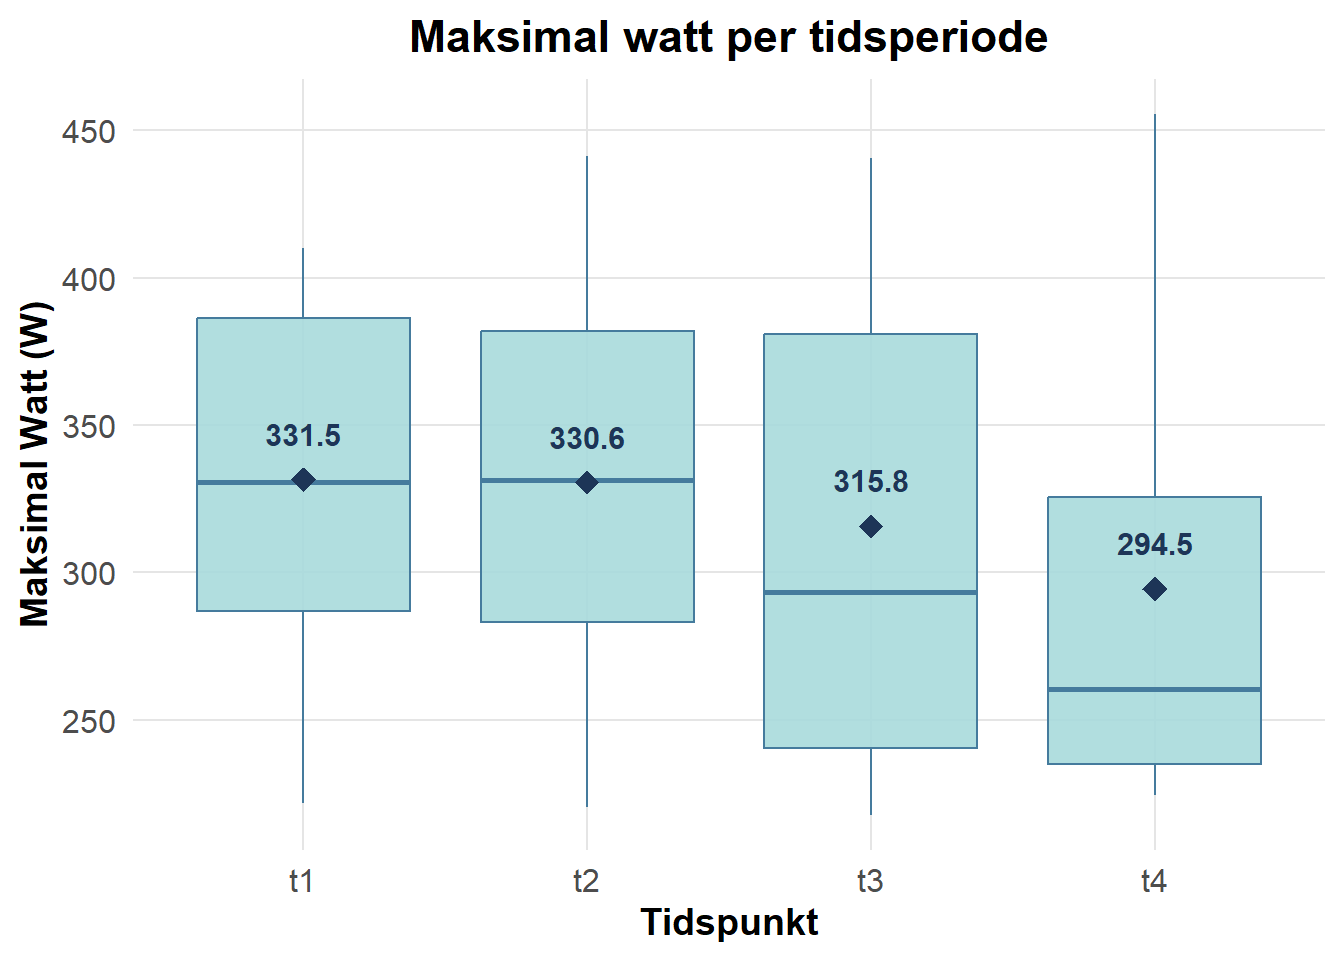
\includegraphics[keepaspectratio]{01-reliabilitet_files/figure-pdf/fig-makswatt-1.pdf}}

}

\caption{\label{fig-makswatt}Gjennomsnittlige watt-verdier for hele
gruppen for hver testforsøk.}

\end{figure}%

For å forstå variasjonene på individnivå, ble maksimal watt analysert
for hver deltaker. Figure~\ref{fig-individ} viser gjennomsnittlig watt
for hver deltaker, sortert fra lavest til høyest, med feilstenger som
representerer typisk feil for å visualisere variasjonen mellom målinger
for hver deltaker. Typisk feil gir en indikasjon på den forventede
variasjonen i watt ved en ny test. Fargekodingen angir enten høy (CV ≤
3\%), moderat (CV \textgreater{} 3\% og ≤ 5\%) og lav (CV \textgreater{}
5\%) reliabilitet (Hopkins (2000)). Generelt viste de fleste
testpersonene høg reliabilitet, mens noen hadde større variasjon og
lavere reliabilitet mellom målingene. Det er viktig å påpeke at
Figure~\ref{fig-individ} kun inkluderer testpersoner som har gjennomført
to eller flere tester, ettersom dette er nødvendig for å kunne beregne
typisk feil \[ 
\text{Typical Error} = \frac{\text{SD of differences}}{\sqrt{2}} 
\]

og CV:
\[ \text{CV (\%)} = \frac{\text{Typical Error}}{\text{Mean Watt}} \times 100 \].

\begin{figure}

\centering{

\pandocbounded{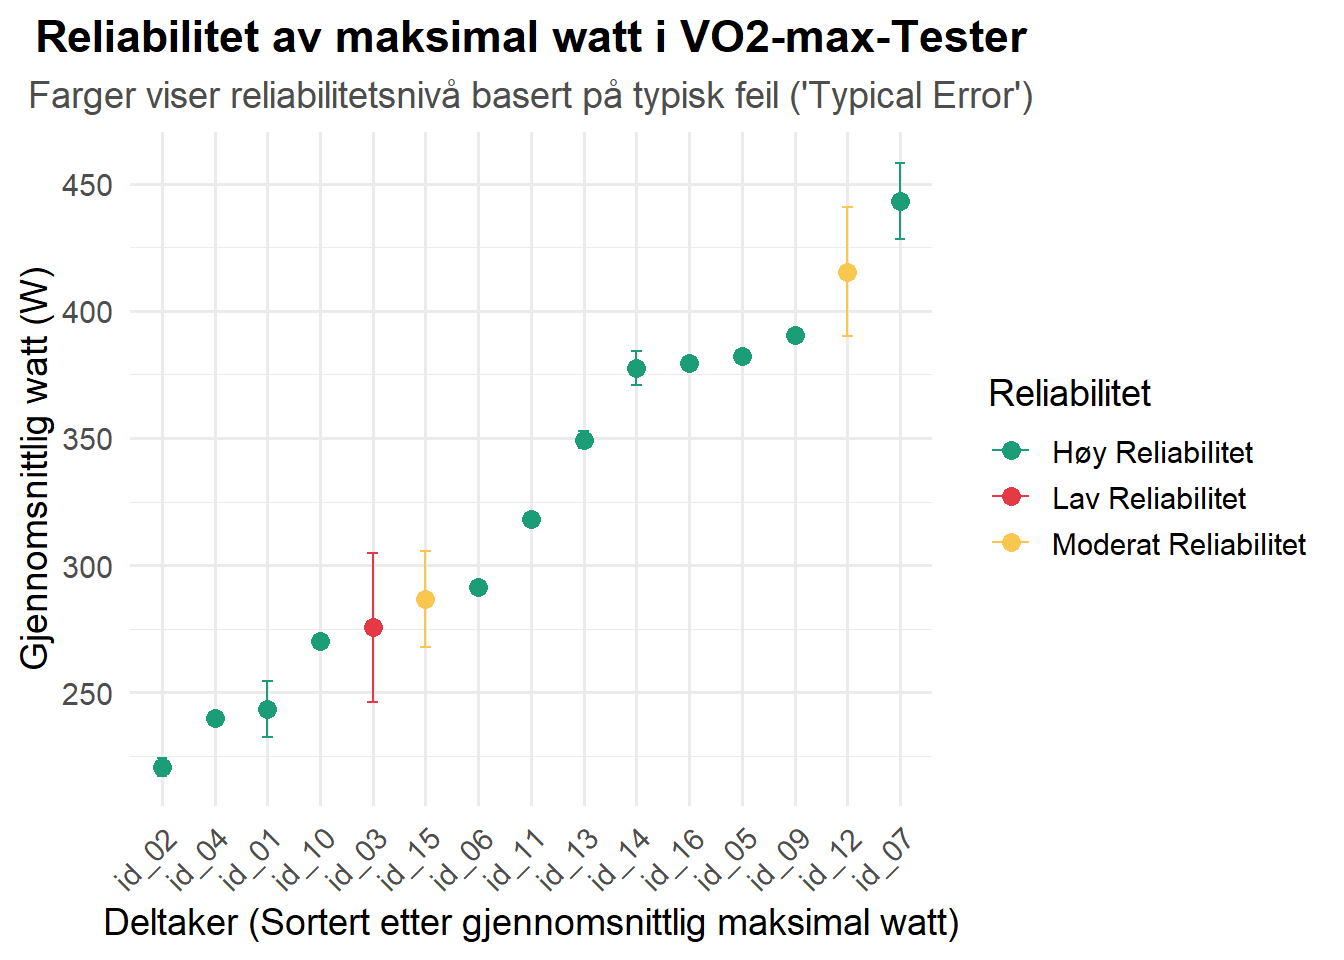
\includegraphics[keepaspectratio]{01-reliabilitet_files/figure-pdf/fig-individ-1.pdf}}

}

\caption{\label{fig-individ}Gjennomsnittlige wattverdier med typisk feil
fra alle testforsøk for samtlige testpersoner.}

\end{figure}%

Table~\ref{tbl-typ-CV} gir en detaljert oversikt over typisk feil og CV
for hver deltaker, beregnet basert på alle tester gjennomført av den
enkelte. De er rangert etter gjennomsnittlig watt, og fargene følger
samme rangering mellom høy (grønn, CV ≤ 3\%), moderat (gul, CV
\textgreater{} 3\% og ≤ 5\%) og lav (rød) (CV \textgreater{} 5\%)
reliabilitet. Som i Figure~\ref{fig-individ}, viser
Table~\ref{tbl-typ-CV} generelt høy reliabilitet blant deltakerne, med
koeffisient av variasjon (CV) ≤ 3 \% for flertallet. Id\_09, id\_11,
id\_16, og id\_10 skiller seg ut med svært lav CV (\textless{} 1 \%),
noe som indikerer konsistente målinger mellom testene. Imidlertid ble
betydelig variasjon observert for id\_03 (CV = 10.50 \%) og id\_12 (CV =
5.08 \%), som begge har lav reliabilitet. Id\_01 og id\_04 ligger i
kategorien moderat reliabilitet med CV mellom 3 \% og 5 \%. Det er verdt
å merke seg at id\_11 ikke viser noen variasjon mellom målingene (CV = 0
\%), som kan indikere perfekt samsvar mellom testene, men bør vurderes
for mulig feilregistrering. Mens id\_08 mangler tilstrekkelige data for
beregning av typisk feil og CV.''

\begin{table}

\caption{\label{tbl-typ-CV}Testpersonenes typiske feil (typical error)
og koeffisient av variasjon (CV).}

\centering{

\caption*{
{\large Sammenligning av typisk feil og CV} \\ 
{\small Hver rad representerer en deltaker}
} 
\begin{tabular*}{\linewidth}{@{\extracolsep{\fill}}lrrr}
\toprule
Deltaker-ID & Gj.snitt watt & Typisk feil & CV (\%) \\ 
\midrule\addlinespace[2.5pt]
id\_07 & 434.90 & 13.53 & {\cellcolor[HTML]{F4A261}{\textcolor[HTML]{000000}{3.11}}} \\ 
id\_12 & 406.90 & 20.68 & {\cellcolor[HTML]{E63946}{\textcolor[HTML]{FFFFFF}{5.08}}} \\ 
id\_09 & 389.10 & 1.52 & {\cellcolor[HTML]{1B9E77}{\textcolor[HTML]{FFFFFF}{0.39}}} \\ 
id\_05 & 386.70 & 4.33 & {\cellcolor[HTML]{1B9E77}{\textcolor[HTML]{FFFFFF}{1.12}}} \\ 
id\_16 & 381.50 & 2.17 & {\cellcolor[HTML]{1B9E77}{\textcolor[HTML]{FFFFFF}{0.57}}} \\ 
id\_14 & 379.50 & 4.04 & {\cellcolor[HTML]{1B9E77}{\textcolor[HTML]{FFFFFF}{1.06}}} \\ 
id\_13 & 346.60 & 4.91 & {\cellcolor[HTML]{1B9E77}{\textcolor[HTML]{FFFFFF}{1.42}}} \\ 
id\_11 & 318.30 & 0.00 & {\cellcolor[HTML]{1B9E77}{\textcolor[HTML]{FFFFFF}{0.00}}} \\ 
id\_15 & 292.90 & 8.73 & {\cellcolor[HTML]{1B9E77}{\textcolor[HTML]{FFFFFF}{2.98}}} \\ 
id\_03 & 290.40 & 30.50 & {\cellcolor[HTML]{E63946}{\textcolor[HTML]{FFFFFF}{10.50}}} \\ 
id\_06 & 286.00 & 5.33 & {\cellcolor[HTML]{1B9E77}{\textcolor[HTML]{FFFFFF}{1.86}}} \\ 
id\_10 & 269.40 & 0.82 & {\cellcolor[HTML]{1B9E77}{\textcolor[HTML]{FFFFFF}{0.31}}} \\ 
id\_01 & 242.70 & 8.99 & {\cellcolor[HTML]{F4A261}{\textcolor[HTML]{000000}{3.71}}} \\ 
id\_04 & 231.00 & 9.00 & {\cellcolor[HTML]{F4A261}{\textcolor[HTML]{000000}{3.90}}} \\ 
id\_08 & 230.00 & NA & {\cellcolor[HTML]{808080}{\textcolor[HTML]{FFFFFF}{NA}}} \\ 
id\_02 & 221.00 & 1.96 & {\cellcolor[HTML]{1B9E77}{\textcolor[HTML]{FFFFFF}{0.89}}} \\ 
\bottomrule
\end{tabular*}

}

\end{table}%

For å evaluere reliabiliteten og konsistensen i målingene over tid, har
det blitt gjort parvise sammenligninger av målinger på to spesifikke
tidspunkter. I Table~\ref{tbl-testpar} så referer testpar til denne
parvise sammenligningen mellom målinger utført på to påfølgende
tidspunkt for samme deltaker. I denne analysen har man sett på første
test og andre test (t1 -\textgreater{} t2), andre test til tredje test
(t2 -\textgreater{} t3) og tredje test til fjerde test (t3
-\textgreater{} t4). Typisk feil og koeffisient av variasjon (CV) har
blitt beregnet basert på forskjellen mellom målingene i hvert par i tråd
med anbefalingene til Hopkins et al.~(2000) (Hopkins (2000), s.11).
Samme fargekode som er blitt brukt i de andre tabellene og figurerne for
å illustrere grad av reliabilitet, er også brukt i tabellen under.

\begin{table}

\caption{\label{tbl-testpar}Gjennomsnittlig typisk feil og CV av alle
testpersonen for hvert testpar.}

\centering{

\caption*{
{\large Typisk feil og koeffisient av variasjon (CV) per testpar} \\ 
{\small Kun basert på w.max for tidspunktene t1, t2, t3 og t4}
} 
\begin{tabular*}{\linewidth}{@{\extracolsep{\fill}}lrr}
\toprule
Testpar & Typisk Feil & Gj.snitt CV (\%) \\ 
\midrule\addlinespace[2.5pt]
t1 -> t2 & 12.59 & {\cellcolor[HTML]{1B9E77}{\textcolor[HTML]{FFFFFF}{2.53}}} \\ 
t2 -> t3 & 29.53 & {\cellcolor[HTML]{E63946}{\textcolor[HTML]{FFFFFF}{5.45}}} \\ 
t3 -> t4 & 8.96 & {\cellcolor[HTML]{F4A261}{\textcolor[HTML]{000000}{4.43}}} \\ 
\bottomrule
\end{tabular*}

}

\end{table}%

Basert på funnene i Table~\ref{tbl-testpar} viste testparet t1
-\textgreater{} t2 lavest CV (2.53 \%), noe som indikerer høy
reliabilitet mellom disse målingene, mens t2 -\textgreater{} t3 hadde
høyest CV (5,45 \%), som tilsier lav reliabilitet og større variasjon.
Antall testpersoner i testparene varierte, med 14 personer for testpar
t1 -\textgreater{} t2, 10 personer for t2 -\textgreater{} t3, og 6
personer for t3 -\textgreater{} t4. Denne variasjonen kan påvirke
beregningene av typisk feil og CV, spesielt i testpar med færre
deltakere. Det er derfor mulig at den lavere reliabiliteten observert
for t3 -\textgreater{} t4 delvis skyldes usikkerhet forårsaket av den
mindre utvalgsstørrelsen.

\section{Diskusjon}\label{diskusjon}

Denne rapporten undersøkte reliabiliteten i målinger av maksimal watt
hentet fra VO2max-maks-tester, med fokus på typisk feil og koeffisienten
av variasjon (CV) som mål på reliabilitet. Resultatene viste generelt
høy reliabilitet, men med variasjon mellom testparene. Dette indikerer
at reliabiliteten kan påvirkes av både biologiske faktorer, som fatigue
og fokus, og teknologiske faktorer, som variasjoner i utstyr eller
testledere.

Typisk feil reflekterer variasjon fra flere kilder, inkludert biologiske
faktorer som tretthet og motivasjon, samt teknologiske faktorer som
kalibrering av utstyr og operatørens tilnærming (Hopkins et al., 2000)
(Hopkins (2000), s.2; Halperin, Pyne, and Martin (2015)). Selv om
standardisering av oppvarming, protokoller og testforhold ble
gjennomført, er det vanskelig å eliminere alle kilder til variasjon.
Typisk feil gir derfor et mål på denne variasjonen ved gjentatte
målinger. I denne analysen ble typisk feil beregnet som standardavviket
av differansen mellom påfølgende målinger, justert med faktoren
\(\sqrt{2}\):

\[
TE = \frac{SD_{\text{diff}}}{\sqrt{2}}
\]

Denne tilnærmingen ble valgt for å fokusere på variasjonen mellom
målinger, uavhengig av gjennomsnittsverdien for maksimal watt (Hopkins
(2000), s.3). Ved å fjerne innflytelsen fra prestasjonsnivået, gir denne
metoden et mer rettferdig grunnlag for å sammenligne reliabiliteten
mellom testparene, særlig når deltakernes prestasjonsnivå varierer.

Selv om typisk feil er nyttig, har den en begrensning: Den øker med
måleverdien, noe som gjør det vanskelig å sammenligne reliabiliteten
mellom deltakere med ulik prestasjonsevne. For eksempel vil en utøver
med høy maksimal watt ha en høyere absolutt typisk feil enn en utøver
med lavere watt (Hopkins (2000)). For å håndtere dette ble koeffisienten
av variasjon (CV) brukt som et supplerende mål:

\[
CV (\%) = \frac{\text{Typical Error}}{\text{Mean}}\times 100
\]

CV er dimensjonsløs og gir et mål på variasjonen i prosent av
gjennomsnittet, noe som gjør det mulig å sammenligne reliabiliteten
mellom deltakere, testforhold og utstyr (Hopkins (2000), 3). Dette var
særlig viktig i denne analysen for å evaluere systematiske forskjeller i
reliabilitet mellom testparene og over tid.

En begrensning er variasjon i antall deltakere mellom testparene, noe
som kan ha påvirket presisjonen i utregninge av typisk feil og CV. For
eksempel var det bare 6 personer som ble brukt i analysen av testpar t3
-\textgreater{} t4, noe som fører til økt usikkerhet i estimatene. I
tillegg vil biologiske og teknologiske faktorer som dagsform, tretthet,
variasjon i kalibrering av utstyr og testleders tilnærming, ha bidratt
til variasjon, til tross for standardisering.

Samtidig som det er flere ting som kan ha påvirket estimatene, vil
standardiseringen som ble gjort minimere for ytre påvirkninger. I
tillegg vil kombinasjonen av typisk feil og CV gi et mer nyansert bilde
av variasjonen i målingene. Bruken av
\(TE = \frac{SD_{\text{diff}}}{\sqrt{2}}\) gir et bedre
sammenligningsgrunnlag for å analysere reliabilitet over tid mellom
ulike testpar, ved å fjerne innflytelsen fra gjennomsnittsverdien.

\section{Konklusjon}\label{konklusjon}

Denne rapporten evaluerte reliabiliteten i målinger av maksimal watt fra
VO2max-maks-tester ved bruk av typisk feil og CV. Analysen viste
generelt høy reliabilitet, men med variasjon mellom testparene som kan
tyde på biologiske og teknologiske faktorer. For å muliggjøre
sammenligning på tvers av testpersonene og over ulike tidspunkter av
testing, ble CV brukt som et dimmensjonsløst mål sammen med typisk feil.
Standardisering av protokoller bidro til å redusere variasjon og øke
reproduserbarheten.

\bookmarksetup{startatroot}

\chapter{Assignment 2: Regression models, predicting from
data}\label{assignment-2-regression-models-predicting-from-data}

\section{Overordnet for rapporten}\label{overordnet-for-rapporten}

Denne oppgaven er delt inn tre separate deler som tar for seg konsepter
innenfor analyse av data og regresjon. I del 1 kalkulerer vi laktat
terskler, og ser nærmere på reliabiliteten mellom to ulike
terskelnivåer. Del 2 bruker vi molekylær data til å predikere størrelsen
på DNA-fragment ved hjelp av en veileder. I del 3 skal vi se nærmere på
om det finnes en lineær sammenheng mellom to valgte variabler fra
datasettet \texttt{hypertrophy}i datapakken \texttt{exscidata}. Hver del
vil ha sin egen introduksjon, metode, resultatdel og diskusjon.

All R-kode som er brukt i denne deloppgaven, er samlet og plassert helt
til slutt i teksten, like før neste deloppgave.

\section{Del 1: Laktat terskler}\label{del-1-laktat-terskler}

\subsection{Introduksjon}\label{introduksjon-1}

Laktatterskel (LT) er en sentral variabel innen treningsfysiologi,
spesielt i utholdenhetsidretter, hvor den brukes til å forutsi
prestasjon, styre intensiteten av treningsøkter og evaluere effekten av
trening (Machado, Nakamura, and Moraes 2012; Poole et al. 2021). LT
representerer den arbeidsintensiteten hvor produksjonen av laktat i
blodet overstiger kroppens evne til å fjerne det, noe som fører til en
akkumulering av laktat i blodet (Poole et al. (2021), s.738). Dette
markerer overgangen fra en stabil til en progressivt økende metabolsk
belastning.

Det finnes mange ulike metoder for å bestemme LT, og en av de mest
brukte er å måle intensitetene ved faste blodlaktatnivåer, som 2 og 4
mmol/L, ved hjelp av regresjonsmodeller som predikerer intensiteten ved
disse verdiene (Kindermann, Simon, and Keul (1979); Tanner and Gore
(2012)). Andre tilnærminger, som ``maximal-deviation method'' (Dmax),
beskrevet av Machado et al.~(2012), tilbyr analyser som kan bedre
reflektere de underliggende metabolske mekanismene som er bestemmende
for prestasjon (Machado, Nakamura, and Moraes 2012).

For å evaluere påliteligheten av disse målmetodene, er det viktig å
vurdere testens reliabilitet. Dette kan kvantifiseres gjennom variasjon
innen samme person, også kjent som ``typical error'', på norsk typisk
feil (Hopkins (2000), s.2). Typisk feil forteller noe om den forventede
variasjonen mellom målinger på samme individ og kan uttrykkes som en
prosentandel av gjennomsnittsverdien, kjent som koeffisienten av
variasjon (CV) (Hopkins (2000), 3). CV er dimmensjonsløs og åpner opp
for muligheten å sammenligne reliabiliteten mellom personer med ulik
prestasjonsevne, og er derfor et relevant mål i denne rapporten.

Laktatterskelen er en viktig fysiologisk parameter for å forstå
sammenhengen mellom treningsintensitet og metabolsk respons. Selv om det
finnes flere metoder for å beregne laktatterskel, er det vanlig å bruke
faste blodlaktatnivåer som referansepunkter, som 2 mmol/L og 4 mmol/L,
for å forutsi treningsintensitet (Wickham 2014, kap. 6). Formålet med
denne deloppgave er å sammenligne reliabiliteten til disse tersklene,
målt som typisk feil i prosent av gjennomsnittet.

På grunn av begrenset datainnsamling fra vårt reliabilitetsforsøk,
benyttes datasettet fra \texttt{cyclingstudy} som grunnlag for analysen.
Dette gir mulighet til å beregne og evaluere reliabiliteten av de to
tersklene og utforske deres egnethet i praksis.

\subsection{Metode}\label{metode-1}

For å ha laktatterskler til å undersøke, ble det benyttet et åpent
datasett \texttt{cyclingstudy}, som inneholdt en rekke fysiologiske
variabler fra en sykkelstudie (Sylta et al. (2016)). Fra dette
datasettet ble det hentet ut informasjon om treningsintensitet, målt i
watt, og blodlaktatkonsentrasjoner. Ved hjelp av lineære og polynomiske
modeller ble det beregnet to laktatterskler, 2 mmol/L og 4 mmol/L, for å
evaluere forholdet mellom treningsintensitet og laktatakkumulering.
Prediksjoner fra hver modell ble brukt til å identifisere wattverdier
nærmest tersklene 2 mmol/L og 4 mmol/L. Den tredjegradspolynomiske
modellen ble valgt for å illustrere resultater i detalj.

Data ble filtrert for en deltaker (subject = 10) ved et bestemt
tidspunkt i studien (pre). Laktatkonsentrasjoner mellom 225 og 375 watt
ble omformet til et langt format for enkel visualisering og analyse.
Laktatnivåene ble analysert for å finne treningsintensiteter nærmest
tersklene 2 mmol/L og 4 mmol/L.

Restverdiene (residuals) fra hver modell ble beregnet for å vurdere hvor
godt modellene beskrev dataene. Disse restverdiene ble visualisert i
Figure~\ref{fig-residualer} for å illustrere modellenes avvik fra de
observerte verdiene ved ulike treningsintensiteter. Viderre ble de ulike
modellene, inkludert lineær, andre-, tredje- og fjerdegradspolynomiske
tilpasninger, brukt for å sammenligne hvordan hver modelle beskriver
sammenhengen mellom watt og blodlaktatkonsentrasjon, grafisk fremstilt i
Figure~\ref{fig-modeller}.

Reliabilitet til tersklene ble analysert ved å beregne typisk feil
\(TE = \frac{SD_{\text{diff}}}{\sqrt{2}}\), som prosentandel av
gjennomsnittsverdien, altså koeffisienten av variasjon (CV)
\(CV (\%) = \frac{\text{Typical Error}}{\text{Mean}}\times 100\).

All datahåndtering, analyse og grafisk fremstilling ble utført i R
(versjon 4.1.1).

\subsection{Resultat}\label{resultat-1}

Figure~\ref{fig-modeller} viser sammenhengen mellom treningsintensitet
(watt) og blodlaktatkonsentrasjon, sammen med tilpasninger basert på
ulike modeller. De observerte dataene er koblet med rette linjer, her
synlig som stiplet linje, som interpolerer mellom puntkene. Tersklene 2
mmol/L (gul) og 4 mmol/L (rød) er markert med horisontale linjer, mens
de vertikale linjene (blå og grønn) markerer hvor tersklene møter den
stiplete linjen på x-aksen, basert på visuell estimering.

\begin{figure}

\centering{

\pandocbounded{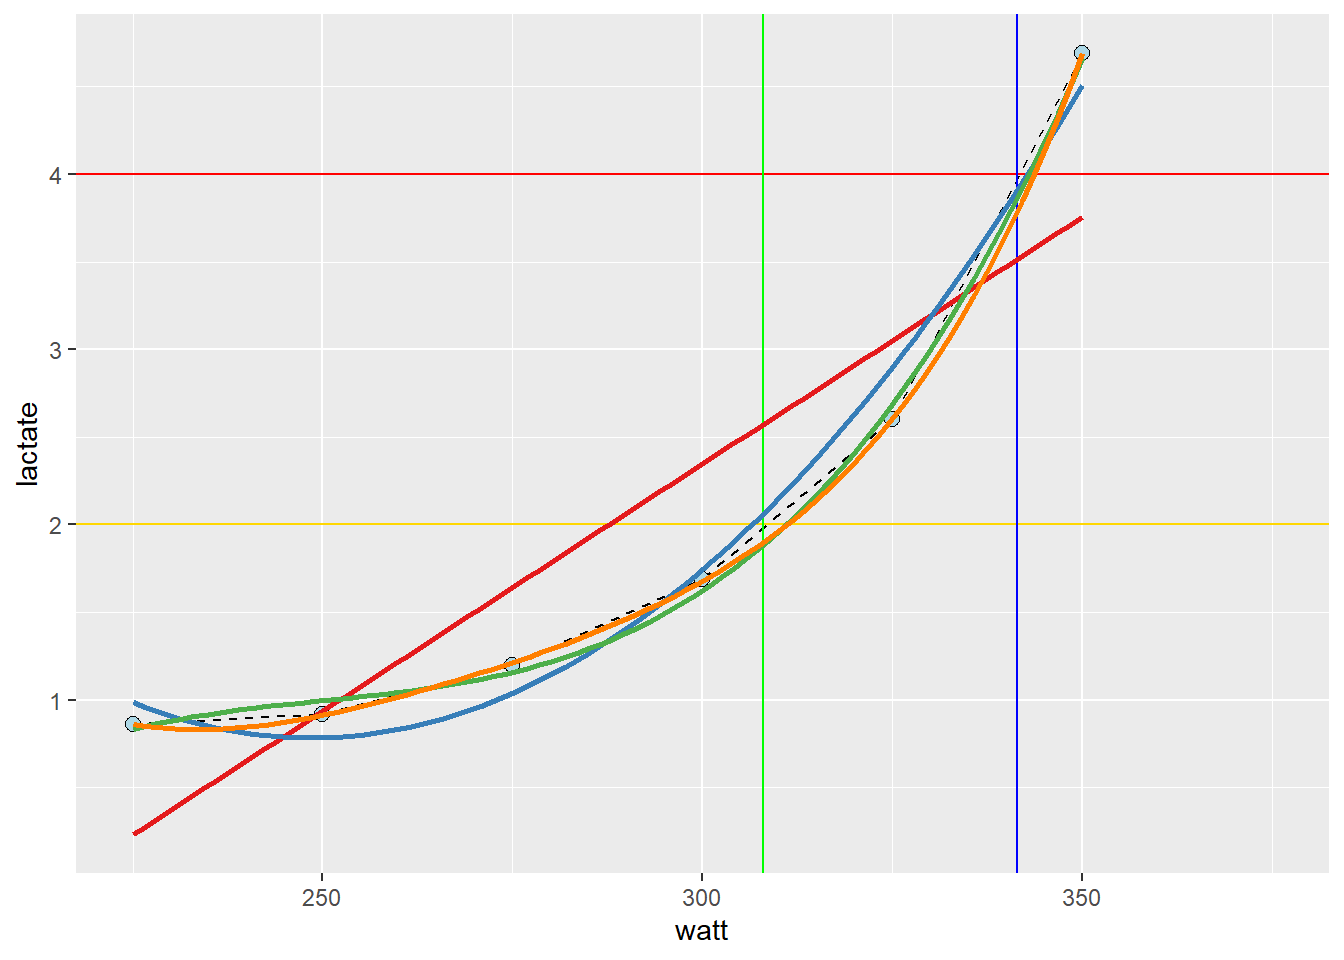
\includegraphics[keepaspectratio]{02-regression-models_files/figure-pdf/fig-modeller-1.pdf}}

}

\caption{\label{fig-modeller}Tilpasning av ulike modeller til
sammenhengen mellom treningsintensitet (watt) og
blodlaktatkonsentrasjon. Grafen viser lineær modell (rød linje),
andregradspolynomisk modell (blå linje), tredjegradspolynomisk modell
(grønn linje), og fjerdegradspolynomisk modell (oransje linje), sammen
med de observerte dataene (punkter). Tersklene ved 2 mmol/L (gul linje)
og 4 mmol/L (rød linje) er indikert.}

\end{figure}%

De ulike modellene ble sammenlignet med hensyn til hvordan de beskriver
dataene, og evaluert ved restverdier (Figure~\ref{fig-residualer}).
Samlet sett gir de tredje- og fjerdegradspolynomiske modellene de beste
tilpasningene, særlig nær tersklene ved 2 mmol/L og 4 mmol/L, mens den
lineære modellen viser større avvik ved høyere wattverdier.
Andregradspolynomiske modellen ligger mellom disse to ytterpuntkene.

\begin{figure}

\centering{

\pandocbounded{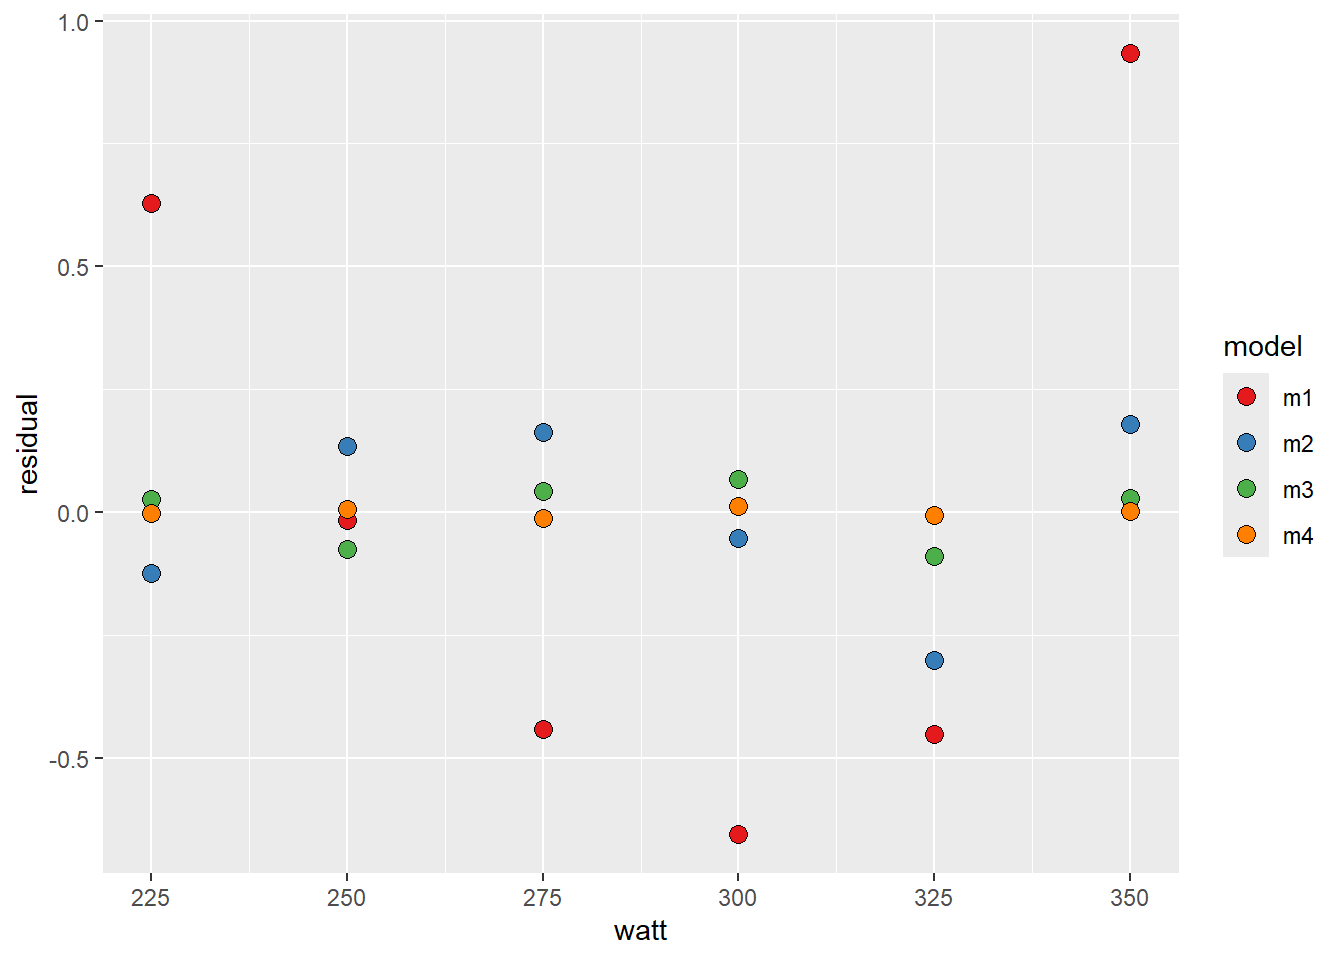
\includegraphics[keepaspectratio]{02-regression-models_files/figure-pdf/fig-residualer-1.pdf}}

}

\caption{\label{fig-residualer}Restverdier for de ulike modellene
(lineær, andregradspolynomisk, tredjegradspolynomisk og
fjerdegradspolynomisk). Grafen viser hvordan modellene avviker fra de
observerte verdiene over treningsintensiteter (watt), med hver modell
representert av forskjellige farger.}

\end{figure}%

Table~\ref{tbl-2mmol} og Table~\ref{tbl-4mmol} viser estimerte watt
verdier ved laktattersklene 2mmol/L og 4 mmol/L, basert på de ulike
modellene. Gjennomsnittet av intensitetene for hver terskel er også
inkludert. Disse predikasjonene ble beregnet ved interpolasjon mellom de
observerte datapunktene for blodlaktatkonsentrasjon.

\begin{table}

\caption{\label{tbl-2mmol}De estimerte treningsintensitetene ved
laktatterksel 2mmol/L basert på de fire ulike modellene: lineær (m1),
andregradspolynomisk (m2), tredjegradspolynomisk (m3), og
fjerdegradspolynomisk (m4).}

\centering{

\caption*{
{\large Laktatterskel ved 2 mmol/L} \\ 
{\small Treningsintensitet per modell og gjennomsnitt}
} 
\fontsize{12.0pt}{14.4pt}\selectfont
\begin{tabular*}{\linewidth}{@{\extracolsep{\fill}}lr}
\toprule
Modell & Treningsintensitet (Watt) \\ 
\midrule\addlinespace[2.5pt]
m1 & 287.7 \\ 
m2 & 306.5 \\ 
m3 & 311.0 \\ 
m4 & 311.1 \\ 
{\bfseries Gjennomsnitt} & {\bfseries 304.1} \\ 
\bottomrule
\end{tabular*}
\begin{minipage}{\linewidth}
Tabellen viser modellene og gjennomsnittet for terskelen ved 2 mmol/L.\\
\end{minipage}

}

\end{table}%

\begin{table}

\caption{\label{tbl-4mmol}De estimerte treningsintensitetene ved
laktatterksel 2mmol/L basert på de fire ulike modellene: lineær (m1),
andregradspolynomisk (m2), tredjegradspolynomisk (m3), og
fjerdegradspolynomisk (m4).}

\centering{

\caption*{
{\large Laktatterskel ved 4 mmol/L} \\ 
{\small Treningsintensitet per modell og gjennomsnitt}
} 
\fontsize{12.0pt}{14.4pt}\selectfont
\begin{tabular*}{\linewidth}{@{\extracolsep{\fill}}lr}
\toprule
Modell & Treningsintensitet (Watt) \\ 
\midrule\addlinespace[2.5pt]
m1 & 350.0 \\ 
m2 & 342.8 \\ 
m3 & 343.0 \\ 
m4 & 343.7 \\ 
{\bfseries Gjennomsnitt} & {\bfseries 344.9} \\ 
\bottomrule
\end{tabular*}
\begin{minipage}{\linewidth}
Tabellen viser modellene og gjennomsnittet for terskelen ved 4 mmol/L.\\
\end{minipage}

}

\end{table}%

Estimatene variere noe mellom modellene for begge terskler. For 2 mmol/L
varierer de fra 287.7 W (lineær modell) til 311.1 W
(fjerdegradspolynomisk), mens snittet ble på 304.1 W. For 4 mmol/L
varierte de fra 342.8 W (andregradspolynomisk modell) til 350 W (lineær
modell), med et snitt på 344.9 W. Dette illustrerer hvordan valg av
modell, spesielt ved høyere intensiteter kan påvirke predikasjonene.

Under i Table~\ref{tbl-reliabilitet}, presenteres mål på reliabilitet
ved tersklene 2 mmol/L og 4 mmol/L. Ved terskel 2 mmol/L har
trenigsintensiteten en høyere typisk feil (7.87 W) og koeffisient av
variasjon (2.59\%) sammenlignet med terskel ved 4 mool/L, hvor typisk
feil og CV\% er henholdsvis 2.43 W og 0.70\%. Man kan derfor antyde at
reliabiliteten er bedre ved høyere terskler (4 mmol/L) enn ved lavere
terskler (2 mmol/L).

\begin{table}

\caption{\label{tbl-reliabilitet}Beregnede verdier av gjennomsnittlig
treningsintensitet (watt), standardavvik for differanser (watt), typisk
feil (watt), og koeffisient av variasjon (CV \%), ved 2 mmol/L og 4
mmol/L}

\centering{

\caption*{
{\large Reliabilitet ved ulike terskler} \\ 
{\small Typisk feil og koeffisient av variasjon}
} 
\fontsize{12.0pt}{14.4pt}\selectfont
\begin{tabular*}{\linewidth}{@{\extracolsep{\fill}}lrrrr}
\toprule
Terskel (mmol/L) & Gjennomsnitt (Watt) & SD Diff (Watt) & Typisk Feil (Watt) & CV (\%) \\ 
\midrule\addlinespace[2.5pt]
2 mmol/L & 304.07 & 11.13 & 7.87 & 2.59 \\ 
4 mmol/L & 344.88 & 3.44 & 2.43 & 0.70 \\ 
\bottomrule
\end{tabular*}
\begin{minipage}{\linewidth}
Tabellen viser beregnet reliabilitet ved tersklene 2 mmol/L og 4 mmol/L.\\
\end{minipage}

}

\end{table}%

\section{Del 2: Forutsi størrelser på DNA fragmenter eller stiningene i
en
qPCR-kalibreringskurve}\label{del-2-forutsi-stuxf8rrelser-puxe5-dna-fragmenter-eller-stiningene-i-en-qpcr-kalibreringskurve}

\subsection{Introduksjon}\label{introduksjon-2}

Sportslige prestasjoner påvirkes av både miljømessige og genetiske
faktorer (Tucker and Collins (2012)). Et viktig gen i denne sammenhengen
er \emph{ACTN3}. som koder for proteinet alpha-actinin-3. Dette
proteinet finnes nesten utelukkende i hurtige muskelfibre og er kjent
for sine rolle i kraftbaserte aktiviteter som sprint og vektløfting
(Mikami et al. (2014); North and Beggs (1996); Schadock et al. (2015)).
Mutasjoner i genet kan føre til en ikke-funksjonell variant, kjent som
R577X-polymorfismen, som resulterer i manglende produksjon av proteinet
(North et al. (1999)). Genotyper som inneholder R allelet, er assosiert
med bedre ytelse i kraftfulle og eksplosive idretter, mens X-allelet kan
være gunstig for utholdenhet (Mikami et al. (2014); Yang et al. (2003),
s.629-630).

For å analysere genotypene til \emph{ACTN3}-genet, vil molekylære
teknikker som PCR (polymerasekjedereaksjon) og elektroforese være
nyttig. PCR muliggjør spesifikk amplifisering av DNA-sekvenser, slik at
man kan identifisere genetiske variasjoner (Schadock et al. (2015)).
Elekttroforese i agarosegel brukes deretter til å separere
DNA-fragmentene basert på størrelse, noe som vil gi en visuell
representasjon av genotypene (Schadock et al. (2015)).

I denne delen av oppgaven ble \emph{ACTN3}-genet undersøkt gjennom
DNA-analyse, som ble gjennomført som en del av et forsøk på
molekylærelaboratoriet. Ved hjelp av PCR og elektroforse forsøkte man å
separere og analyser fragmentstørrelsene til \emph{ACTN3}-genet for å
kartlegge genotypen i de ulike prøvene, for å innsikt i genetiske bidrag
til fysisk ytelse og idrettsprestasjoner.

\subsection{Metode}\label{metode-2}

\subsubsection{DNA-ekstraksjon}\label{dna-ekstraksjon}

DNA ble ekstrahert fra blodprøver samlet i prøverør med EDTA
(etylendiamintetraeddiksyre) ved hjelp av en modifisert protokoll basert
på Bartlett og Stirling (Bartlett and Stirling (2003), kap 6). Etter
overføringen av 3 mL blod til et 15 mL rør, ble cellene lysert med
Reagens A og sentrifugert (3000 g i 5 min) for å isolere en cellepellet.
Pelleten ble resuspendert i Reagens B, og DNA ble frigjort ved
tilsetning av natriumperklorat (250 μl av 5 M sodium perchlorate) og
inkubasjon ved 65 °C. Etter avkjøling i romtemperatur, ble iskald
kloroform (2 mL) tilsatt for å skille DNA fra andre cellekomponenter, og
mikset i en roterende misker i mellom 30 til 60 min. Etterpå ble den
sentrifugert etterfulgt av sentrifugering (2400 g i 2 min) for å hente
ut den øvre delen av prøven. DNA ble uthentet med kald 100\% etanol (2-3
mL), tørket og resuspendert i TE-buffer (200 ul). Konsentrasjonen ble
målt med et spektrofotometer, og verdiene låg rundt 200 og 500 ng/ul.

\subsubsection{\texorpdfstring{Bestemmelse av
\emph{ACTN3}-genotypen}{Bestemmelse av ACTN3-genotypen}}\label{bestemmelse-av-actn3-genotypen}

\emph{ACTN3}-genotypen ble bestemt ved bruk av en fire-primer
PCR-protokoll tilpasset fra Schadock et al.~(2015) (Schadock et al.
(2015)). PCR-reaksjonen ble satt opp i et totalvolum på 20 µL, bestående
av 10 µL 2X master mix, 5 µL primermiks (inneholdt hsACTN3\_F1,
hsACTN3\_R1, hsACTN3Tif\_F2, og hsACTN3Cir\_R2) og 5 µL DNA-prøve (se
over). PCR-syklusen inkluderte initial denaturering ved 95 °C i 2
minutter, etterfulgt av 35 sykluser med 95 °C i 10 sekunder, og 72 °C i
45 sekunder, og til slutt ved 72 °C i 2 minutter.

\subsubsection{Elektroforese for analyse av
PCR-produkter}\label{elektroforese-for-analyse-av-pcr-produkter}

PCR-produktene ble analysert ved hjelp av agarosegelektroforese i en 2
\% agrosegel. Gelen ble fremstilt ved å løse 2 g agarose i 100 mL 1X
TBE-buffer, med tilsetning av 10 µL Sybr Safe for visualisering av DNA.
Løsningen ble oppvarmet til klarhet, avkjølt til cirka 60 grader, og
deretter helt i en støpeform med gelkammer. Etter cirka 1 time hadde
gelet blitt fast, og ble plassert i en horisontal elektroforeseenhet
fylt med 1X TBE-buffer

DNA-prøvene ble blandet med 6X farge (1 µL per 5 µL DNA-prøve), og 2-5
µL av hver prøve ble lastet i egne brønner sammen med en DNA-stige som
referanse. Eletroforesen ble utført ved 150 V i cirka 1 time, inntil
fargeindikatoren hadde vandret rundt 80\% av gelens lengde. Gelen med
prøvene ble visualisert i en G ved bruk av UV-lys og Sybr
Green-instillinger.

\subsubsection{Analyse av PCR-produkter med Iamge J og
R}\label{analyse-av-pcr-produkter-med-iamge-j-og-r}

For å bestemme størrelsen på PCR-produktene ble bildeanalyse utført med
IamgeJ Fiji. Gelbildet ble invertert, rotert og trimmet for å isolere
prøvene og DNA-stigen. Ved bruk av rektangelverktøyet ble stigen og
prøvene markert, og toppunktene i intensitetsgrafene ble registret.
Disse punktene representerte DNA-fragmentenees migrasjonsavstand, og
dataene ble eksportert til Excel for videre analyse.

I R ble en kalibreringskurve laget basert på DNA-stigen
(Figure~\ref{fig-kali}), hvor logaritmen av molekylvekten ble plottet
mot migrasjonsavstanden. Kalibrering ble utført ved hjelp av en
polynommodell for å sikre høy presisjon. Denne modellen ble deretter
brukt til å estimere molekylstørrelsen for de ukjente prøvene. Modellen
ble vurdert basert på \(R^2\)-verdien fra lineær regresjon, og verdien
lå nær 1, noe som indikerte høy modellpresisjon. Den justerte modellen
ble deretter brukt til å estimere molekylstørrelsene for de ukjente
prøvene, som ble beregnet på migrasjonsavstandene fra gelelektroforesen.

\begin{figure}

\centering{

\pandocbounded{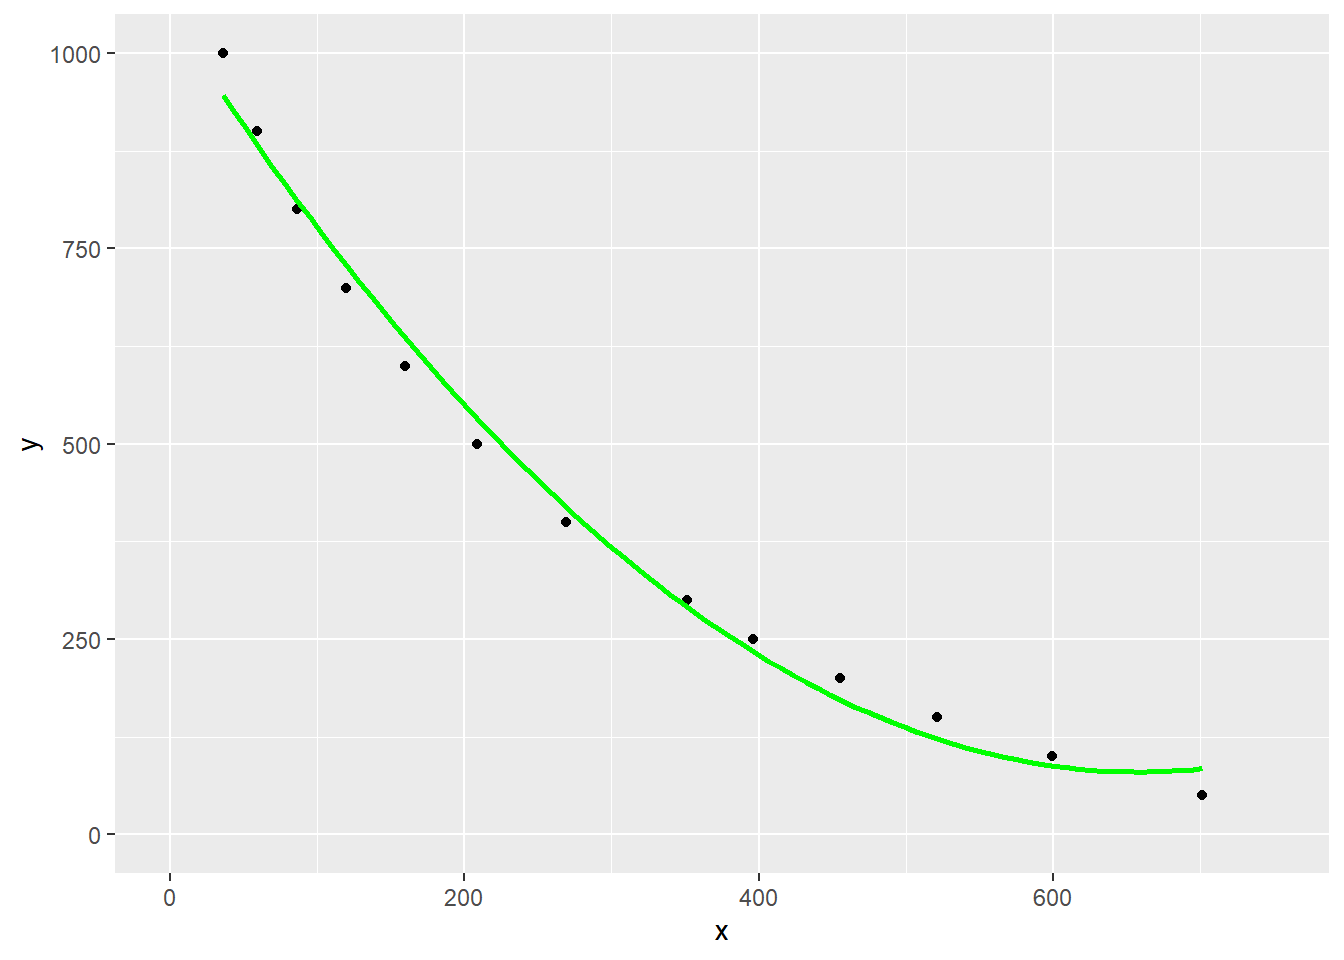
\includegraphics[keepaspectratio]{02-regression-models_files/figure-pdf/fig-kali-1.pdf}}

}

\caption{\label{fig-kali}Kalibreringskurve basert på DNA-stigen.}

\end{figure}%

\begin{verbatim}

Call:
lm(formula = log(mw) ~ dist, data = ladder)

Residuals:
      Min        1Q    Median        3Q       Max 
-0.244363 -0.040218 -0.004565  0.082943  0.112630 

Coefficients:
              Estimate Std. Error t value Pr(>|t|)    
(Intercept)  7.0915695  0.0480419  147.61  < 2e-16 ***
dist        -0.0041842  0.0001298  -32.23 3.06e-12 ***
---
Signif. codes:  0 '***' 0.001 '**' 0.01 '*' 0.05 '.' 0.1 ' ' 1

Residual standard error: 0.09807 on 11 degrees of freedom
Multiple R-squared:  0.9895,    Adjusted R-squared:  0.9886 
F-statistic:  1039 on 1 and 11 DF,  p-value: 3.059e-12
\end{verbatim}

\subsection{Resultater}\label{resultater}

Analyse av PCR-produktene viste at DNA-fragmentet i brønn 1 (prøve 1)
hadde en estimert båndstørrelse på 407 bp, mens brønn 2 (prøve 2) viste
et fragment på 401 bp. I brønn 3 (prøve 3) ble det identifisert to
fragmenter, med størrelser på henholdsvis 396 bp og 296
(Table~\ref{tbl-DNA}). Disse resultatene ble beregnet basert på
kalibreringskurven som ble laget ved hjelp av DNA-stigen, og
fragmentstørrelsene reflekterer migrasjonsmønsteret observert i
gelanalysen.

\begin{table}

\caption{\label{tbl-DNA}Resultater fra PCR-analyse: Estimert
båndstørrelse for DNA-fragmenter basert på agarosegelelektroforese.}

\centering{

\caption*{
{\large Resultater fra PCR-analyse}
} 
\fontsize{12.0pt}{14.4pt}\selectfont
\begin{tabular*}{\linewidth}{@{\extracolsep{\fill}}rr}
\toprule
Brønn & Båndstørrelse (bp) \\ 
\midrule\addlinespace[2.5pt]
1 & 407 \\ 
2 & 401 \\ 
3 & 396, 296 \\ 
\bottomrule
\end{tabular*}

}

\end{table}%

\subsection{Diskusjon}\label{diskusjon-1}

Denne analysen viste at ingen av DNA-fragmentene hadde nøyaktig den
forventede størrelsen på 413 bp (R/R) eller 318 bp (X/X) (Schadock et
al. (2015)). Fragmentene fra brønn 1 (417bp) og brønn 2 (401 bp) ligger
imidlertid nær den forventede størrelse for R/R-genotypen, mens brønn 3
(396 bp og 296 bp) indikerer en mulig heterozygot genotype (R/X)
(Schadock et al. (2015)). Avvikene kan forklares med flere faktorer,
inkludert tekniske og menneskelige feil under eksperimentet.

Blant de tekniske feilene er kvaliteten på gelbildet noe som kan ha
bidratt til usikkerhet i målingene, ettersom dårlig oppløsning eller
utilstrekkelig kontrast gjør det vanskelig å nøyaktig identifisere
båndenes plassering. Videre kan kalibreringsmodellen ha blitt påvirket
av små feil i dataregistreringen, noe som kan ha påvirket nøaykatigheten
i estimeringen av fragmentstørrelsene.

Menneskelige feil er også en viktig faktor å vurdere. Feil pipetering
kan ha ført til variasjon i mengden DNA eller reagenser, noe som kan
påvirke amplifiseringen. Under elektroforese kan små variasjoner i
prøvelasting, som ulik mengde DNA-prøve i brønnene, ha forårsaket
skjevheter i båndenes intensitet og plassering. I tillegg kan subjektiv
tolkning av gelbilder uten digitale analyseverktøy føre til
feiltolkninger.

Denne oppgaven viste at PCR-analysen ga fragmenter som lå nær forventede
størrelser, men med mindre avvik, noe som kan tilskrives både tekniske
og menneskelige feil. Dette understreker viktigheten av presisjon i
laboratoriearbeid og bruk av objektive metoder for dataanalyse.

\section{Del 3: Tolkning av
regresjonsmodell}\label{del-3-tolkning-av-regresjonsmodell}

\subsection{Introduksjon}\label{introduksjon-3}

Muskeltilpasninger til trening avhenger av en kompleks kombinasjon av
genetiske og miljømessige faktorer. Myonuclei (cellkjerner), som finnes
i muskelfibrene, spiller en nøkkelrolle i å regulere musklenes kapasitet
for proteinsyntese og dermes også evnen til å utvikle styrke og kraft
(McArdle, Katch, and Katch 2014, kap 22). Antall myonuclei i type-II
muskelfibre er spesielt relevant, da disse fibrene er avgjørende for
eksplosive bevegelser og maksimal styrke (McArdle, Katch, and Katch
2014, kap 22). Samtidig er det uklart i hvilken grad treningserfaring,
mål som antall år med systematisk trening, kan påvirke antallet
myonuclei (McArdle, Katch, and Katch 2014, s.535).

Ved å undersøke sammenhengen mellom antall myonuclei i type II
muskelfibre og treningsalder, kan man belyse om langvarig trening har en
målbar effekt på muskelfiberens egenskaper. Dette kan gi innsikt som er
relevant både for praktisk trening og for å forstå mekanismene bak
muskeltilpasning.

\textbf{Spørsmålet}: Finnes det en lineær sammenheng mellom antall
myonuclei per type-II muskelfiber og treningsalder?

\subsection{Metode}\label{metode-3}

For å undersøke sammenhengen mellom antall myonuclei per type-II
muskelfiber og treningsalder, brukte såg man på variablene
\texttt{FAST\_NUCLEI\_T1} og \texttt{TRAINING\_AGE} i datasettet
\texttt{hypertrofi} fra \texttt{exscidata}-pakken. Lineær regresjon ble
benyttet, da denne er velegnet for å evaluere en potensiell lineær
relasjon mellom en avhengig variabel (\texttt{FAST\_NUCLEI\_T1}) og en
uavhengig variabel (\texttt{TRAINING\_AGE}) (Spiegelhalter 2019,
s.128--129).

Datasettet ble først filtrert for å ekskludere observasjoner med
manglende verdier, og vi valgte kun de relevante variablene for
analysen. Dataene ble deretter visualisert med scatterplott og en
tilhørende regresjonslinje generert av \texttt{geom\_smooth}, se
Figure~\ref{fig-plot-training-age-myonuclei}. Regresjonslinjen gir en
indikasjon på hvordan variablene relaterer seg til hverandre, mens det
gråe konfidensintervallet rundt linjen reflekterer usikkerheten i
modellen. Et bredt konfidensintervall, som sett her, indikerer større
usikkerhet i forholdet mellom variablene (Spiegelhalter 2019,
s.240--244).

\begin{Shaded}
\begin{Highlighting}[]
\CommentTok{\# Laster inn nødvendige biblioteker}
\FunctionTok{library}\NormalTok{(exscidata)}
\FunctionTok{library}\NormalTok{(tidyverse)}
\FunctionTok{library}\NormalTok{(gt)}
\FunctionTok{library}\NormalTok{(broom)}

\CommentTok{\# Laster inn data}
\FunctionTok{data}\NormalTok{(}\StringTok{"hypertrophy"}\NormalTok{)}

\CommentTok{\# Filtrerer ut NA{-}verdier før du velger variabler}
\NormalTok{ds }\OtherTok{\textless{}{-}}\NormalTok{ hypertrophy }\SpecialCharTok{\%\textgreater{}\%}
  \FunctionTok{filter}\NormalTok{(}\SpecialCharTok{!}\FunctionTok{is.na}\NormalTok{(TRAINING\_AGE) }\SpecialCharTok{\&} \SpecialCharTok{!}\FunctionTok{is.na}\NormalTok{(FAST\_NUCLEI\_T1)) }\SpecialCharTok{\%\textgreater{}\%}
  \FunctionTok{select}\NormalTok{(PARTICIPANT, GROUP, TRAINING\_AGE, FAST\_NUCLEI\_T1)}

\CommentTok{\# Plotter data uten NA{-}verdier}
\NormalTok{ds }\SpecialCharTok{\%\textgreater{}\%} 
  \FunctionTok{ggplot}\NormalTok{(}\FunctionTok{aes}\NormalTok{(TRAINING\_AGE, FAST\_NUCLEI\_T1)) }\SpecialCharTok{+}
  \FunctionTok{geom\_point}\NormalTok{(}\AttributeTok{size =} \DecValTok{2}\NormalTok{, }\AttributeTok{fill =} \StringTok{"red"}\NormalTok{) }\SpecialCharTok{+}
  \FunctionTok{geom\_smooth}\NormalTok{(}\AttributeTok{method =} \StringTok{"lm"}\NormalTok{, }\AttributeTok{se =} \ConstantTok{TRUE}\NormalTok{) }\SpecialCharTok{+}
  \FunctionTok{labs}\NormalTok{(}
    \AttributeTok{title =} \StringTok{"Sammenheng mellom treningserfaring og myonuklei"}\NormalTok{,}
    \AttributeTok{x =} \StringTok{"Treningsår"}\NormalTok{, }
    \AttributeTok{y =} \StringTok{"Myonuklei per fiber CSA i Type II"}\NormalTok{) }\SpecialCharTok{+}
  \FunctionTok{theme\_minimal}\NormalTok{()}
\end{Highlighting}
\end{Shaded}

\begin{figure}[H]

\centering{

\pandocbounded{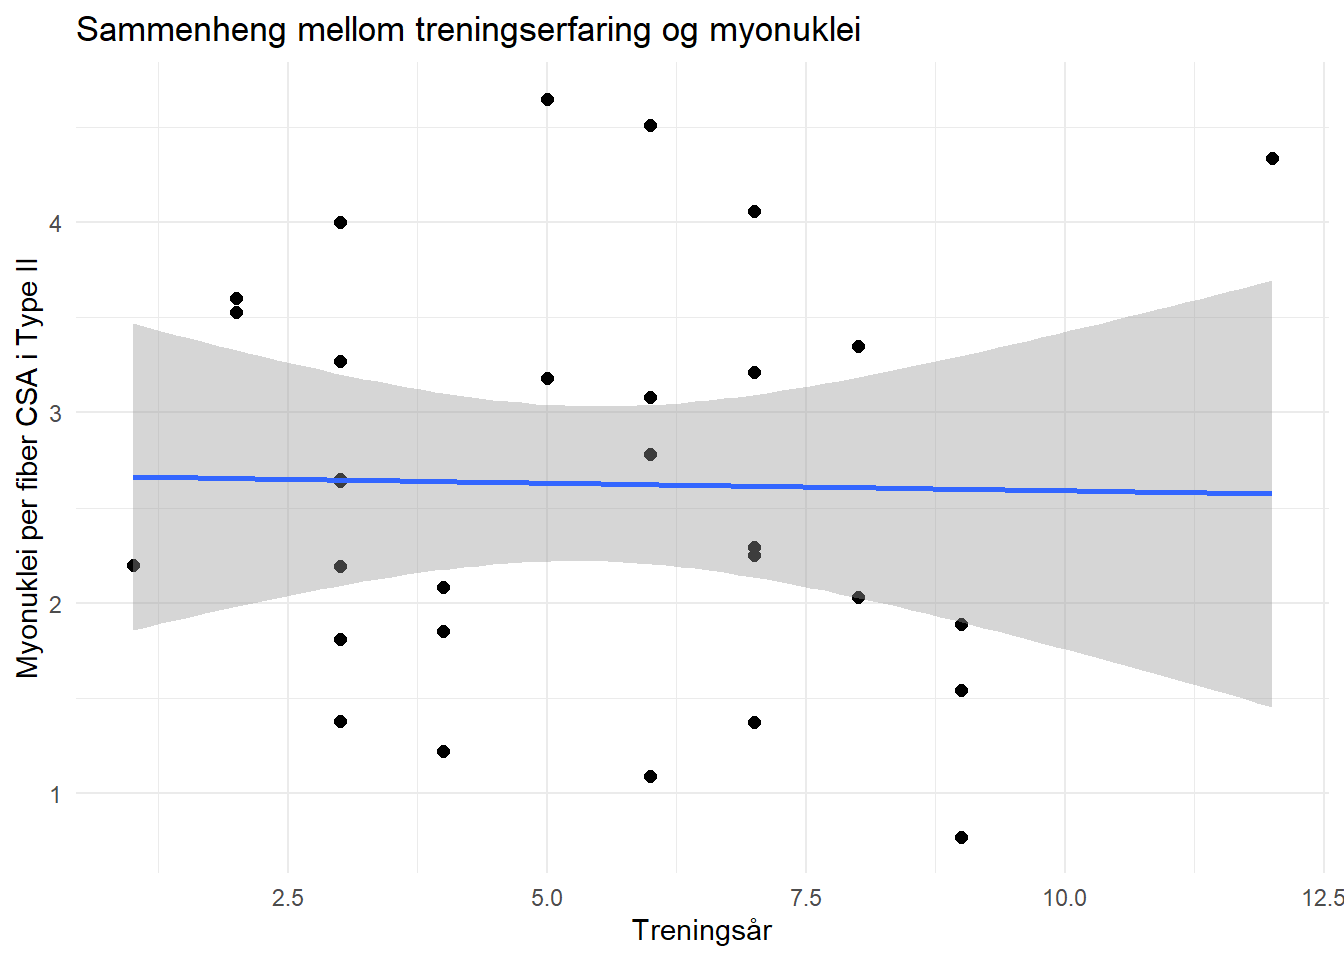
\includegraphics[keepaspectratio]{02-regression-models_files/figure-pdf/fig-plot-training-age-myonuclei-1.pdf}}

}

\caption{\label{fig-plot-training-age-myonuclei}Sammenheng mellom
treningalder og myonuclei per fiber CSA i Type-II}

\end{figure}%

\subsection{Resultat}\label{resultat-2}

Tabellen i Table~\ref{tbl-regresjon} oppsummerer de statistiske
parametrene fra den lineære modellen, inkludert den estimerte
koeffisenten, standardfeilen, \emph{t}-verdien og \emph{p}-verdien.
Disse komponentene gir innsikt i styrken og usikkerheten rundt
sammenhengen mellom variablene. Intercept ble ekskludert fra tabellen,
da det representerer vedien av den avhengige variabelen når den
uavhengige variabelen er null, noe som ikke er relevant for denne
analysen.

\begin{table}

\caption{\label{tbl-regresjon}Sammenheng mellom treningserfaring og
myonuklei per muskelfiber type-II}

\centering{

\begin{Shaded}
\begin{Highlighting}[]
\CommentTok{\# Lager lineær modell med ds uten NA{-}verdier}
\NormalTok{mod1 }\OtherTok{\textless{}{-}} \FunctionTok{lm}\NormalTok{(FAST\_NUCLEI\_T1 }\SpecialCharTok{\textasciitilde{}}\NormalTok{ TRAINING\_AGE, }\AttributeTok{data =}\NormalTok{ ds)}

\CommentTok{\# Henter ut koeffisienter og deres statistikker}
\NormalTok{model\_summary }\OtherTok{\textless{}{-}} \FunctionTok{tidy}\NormalTok{(mod1)}

\CommentTok{\# Tilpasser p{-}verdier og runder av, og fjerner interceptet}
\NormalTok{model\_summary }\OtherTok{\textless{}{-}}\NormalTok{ model\_summary }\SpecialCharTok{\%\textgreater{}\%}
  \FunctionTok{mutate}\NormalTok{(}
    \AttributeTok{term =} \FunctionTok{ifelse}\NormalTok{(term }\SpecialCharTok{==} \StringTok{"(Intercept)"}\NormalTok{, }\StringTok{"Intercept (Konstantledd)"}\NormalTok{, }\StringTok{"Treningserfaring (år)"}\NormalTok{),}
    \AttributeTok{p.value =} \FunctionTok{ifelse}\NormalTok{(p.value }\SpecialCharTok{\textless{}} \FloatTok{0.001}\NormalTok{, }\StringTok{"\textless{} 0.001"}\NormalTok{, }\FunctionTok{round}\NormalTok{(p.value, }\DecValTok{3}\NormalTok{)),}
    \AttributeTok{estimate =} \FunctionTok{round}\NormalTok{(estimate, }\DecValTok{3}\NormalTok{),}
    \AttributeTok{std.error =} \FunctionTok{round}\NormalTok{(std.error, }\DecValTok{3}\NormalTok{),}
    \AttributeTok{statistic =} \FunctionTok{round}\NormalTok{(statistic, }\DecValTok{3}\NormalTok{)}
\NormalTok{  ) }\SpecialCharTok{\%\textgreater{}\%}
  \CommentTok{\# Filtrer ut interceptet}
  \FunctionTok{filter}\NormalTok{(term }\SpecialCharTok{!=} \StringTok{"Intercept (Konstantledd)"}\NormalTok{)}
  \CommentTok{\# Velger å filtrere ut intercept da det ikkje er aktuelt når vi kun skal se om}
  \CommentTok{\# det er en lineær sammenheng mellom dei to variablene}

\CommentTok{\# Lager regresjonstabell med forklarende radnavn}
\NormalTok{regression\_table }\OtherTok{\textless{}{-}}\NormalTok{ model\_summary }\SpecialCharTok{\%\textgreater{}\%}
  \FunctionTok{select}\NormalTok{(term, estimate, std.error, statistic, p.value) }\SpecialCharTok{\%\textgreater{}\%}
  \FunctionTok{gt}\NormalTok{() }\SpecialCharTok{\%\textgreater{}\%}
  \FunctionTok{fmt\_auto}\NormalTok{() }\SpecialCharTok{\%\textgreater{}\%}
  \FunctionTok{cols\_label}\NormalTok{(}
    \AttributeTok{term =} \StringTok{"Term"}\NormalTok{,}
    \AttributeTok{estimate =} \StringTok{"Estimert koeffisient"}\NormalTok{,}
    \AttributeTok{std.error =} \StringTok{"Standardfeil"}\NormalTok{,}
    \AttributeTok{statistic =} \FunctionTok{md}\NormalTok{(}\StringTok{"*t*{-}verdi"}\NormalTok{),}
    \AttributeTok{p.value =} \FunctionTok{md}\NormalTok{(}\StringTok{"*p*{-}verdi"}\NormalTok{)}
\NormalTok{  ) }\SpecialCharTok{\%\textgreater{}\%}
  \FunctionTok{tab\_source\_note}\NormalTok{(}
    \AttributeTok{source\_note =} \StringTok{"Notat: p{-}verdier mindre enn 0.05 anses som statistisk signifikante."}
\NormalTok{  )}

\CommentTok{\# Vis resultatene}
\NormalTok{regression\_table}
\end{Highlighting}
\end{Shaded}

\fontsize{12.0pt}{14.4pt}\selectfont
\begin{tabular*}{\linewidth}{@{\extracolsep{\fill}}lrrrr}
\toprule
Term & Estimert koeffisient & Standardfeil & \emph{t}-verdi & \emph{p}-verdi \\ 
\midrule\addlinespace[2.5pt]
Treningserfaring (år) & -0.008 & 0.077 & -0.104 & 0.918 \\ 
\bottomrule
\end{tabular*}
\begin{minipage}{\linewidth}
Notat: p-verdier mindre enn 0.05 anses som statistisk signifikante.\\
\end{minipage}

}

\end{table}%

\subsection{Diskusjon}\label{diskusjon-2}

I tabellen kan vi lese av verdiene for estimert koeffisient
(regresjonskoeffisient), standardfeil, t-verdi og p-verdi. Den estimerte
koeffisenten til ``Treningserfaring (år)'' indikerer at
\texttt{FAST\_NUCLEI\_T1} reduseres med 0.008 per år med
treningserfaring. Denne negative endringen er imidletid svak, og
standardfeilen er relativt stor i forhold til koeffisienten, noe som
tyder på at estimatet er usikkert (Spiegelhalter 2019, s.230--232)

Standardfeilen gir en indikasjon på hvor mye koeffisienten kan forventes
å mellom ulike utvalg (Spiegelhalter 2019, s.230--232). Selv om
standardfeilen numerisk er lav, er dens forhold til koeffisienten
avgjørende for tolkningen. I dette tilfellet bør man være forsiktig med
å trekke konklusjoner om nøyaktigheten til estimatet.

\emph{t-verdien} sier hvor mange standardavvik den estimerte
koeffisienten er fra null. En større t-verdi, enten negativ eller
positiv, tyder på at man med større sikkerhet kan si at koeffisienten er
signifikant (Spiegelhalter 2019, s.275--276). Med en t-verdi på -0.104,
i vårt tilfelle, kan man ikke med sikkerhet si at det er en signifikant
lineær sammenheng mellom \texttt{FAST\_NUCLEI\_T1} og
\texttt{TRAINING\_AGE}.

\emph{p-verdien} er nært knyttet til t-verdien, og hjelper oss å vurdere
om t-verdien er statistisk signifikant. P-verdien representerer
sannsynligheten for å observere en teststatistikk som er like ekstrem
,eller like ekstrem, som den t-verdien vi har fått, gitt antagelsen at
det ikke er en sammenheng mellom variablene våre (Spiegelhalter 2019,
s.264--265). I vår modell er p-verdien 0.918, noe som tilsier at det er
91,8 \% sannsynlighet at man vil observere en t-verdi på -0.008, gitt
nullhypotesen. Dermed kan man ikke konkludere med at den uavhengige
variabelen TRAINING\_AGE har en effekt på den avhengige variabelen
FAST\_NUCLEI\_T1 eller at det finnes en signifikant lineær sammenheng
mellom disse variablene (Spiegelhalter 2019, s.265--268).

Det er viktig å understreke at p-verdien kun sier noe om den statistiske
signifikansen av resultatene, og ikke om størrelsen på effekten eller
dens praktiske relevans (Spiegelhalter 2019, s.285). I små datasett, som
i vårt tilfelle, kan p-verdien være høy selv om det er en reel effekt,
fordi små utvalg har lavere statistisk styrke til å påvise sammenhenger
(Spiegelhalter 2019, s.285).

Denne analysen har undersøkt sammenhengen mellom treningserfaring og
antall myonuclei per type II-muskelfiber, men resultatene viser ingen
signifikant lineær sammenheng mellom variablene. Selv om p-verdien
indikerer manglende statistisk signifikans, er det viktig å merke seg
begrensningene ved små datasett og mulig usikkerhet knyttet til
estimatene.

\bookmarksetup{startatroot}

\chapter{Assignment 3: Drawing inference from statistical models, and
statistical
power}\label{assignment-3-drawing-inference-from-statistical-models-and-statistical-power}

\bookmarksetup{startatroot}

\chapter{Introduksjon}\label{introduksjon-4}

Denne rapporten er basert på simuleringar utført i R, der resultata blir
analysert gjennom svar på de spesifiserte spørsmåla (1--8). Gjennom
grundig analyse og tolking av resultata gir rapporten ei forklaring som
belyser de viktigaste funna frå simuleringane.

\bookmarksetup{startatroot}

\chapter{Simulering til oppgåve
1-4}\label{simulering-til-oppguxe5ve-1-4}

For å kunne svare på spørsmålene 1 til 4 så er det blitt gjort mange
simuleringer med to ulike utvalgsstørrelser (n =8 og n = 40), som danner
grunnlaget for to lineære modeller, \texttt{m1} og \texttt{m2}. De
viktigste parametrene for modellene er vist i Table~\ref{tbl-modeller}.

\begin{table}

\caption{\label{tbl-modeller}Oversikt over de parametrene som vil bli
diskutert videre i oppgaven.}

\centering{

\caption*{
{\large Parametere for modellene m1 og m2}
} 
\fontsize{12.0pt}{14.4pt}\selectfont
\begin{tabular*}{\linewidth}{@{\extracolsep{\fill}}lrr}
\toprule
Parameter & m1 & m2 \\ 
\midrule\addlinespace[2.5pt]
Estimat & 1.8397275 & 1.564160975 \\ 
Standardfeil & 1.2512930 & 0.477411701 \\ 
t-verdi & 1.4702611 & 3.276335647 \\ 
p-verdi & 0.1849546 & 0.002212965 \\ 
\bottomrule
\end{tabular*}

}

\end{table}%

Under i Figure~\ref{fig-samp1} vises t-fordelingen av de ulike lineære
modellene, der det skyggelagte området visualiserer sannsynligheten for
å observere en t-verdi som er like ekstrem eller mer ekstrem enn den
observerte t-verdien i \texttt{samp1}, gitt at nullhypotesen om ingen
endring er sann.

\begin{figure}

\centering{

\pandocbounded{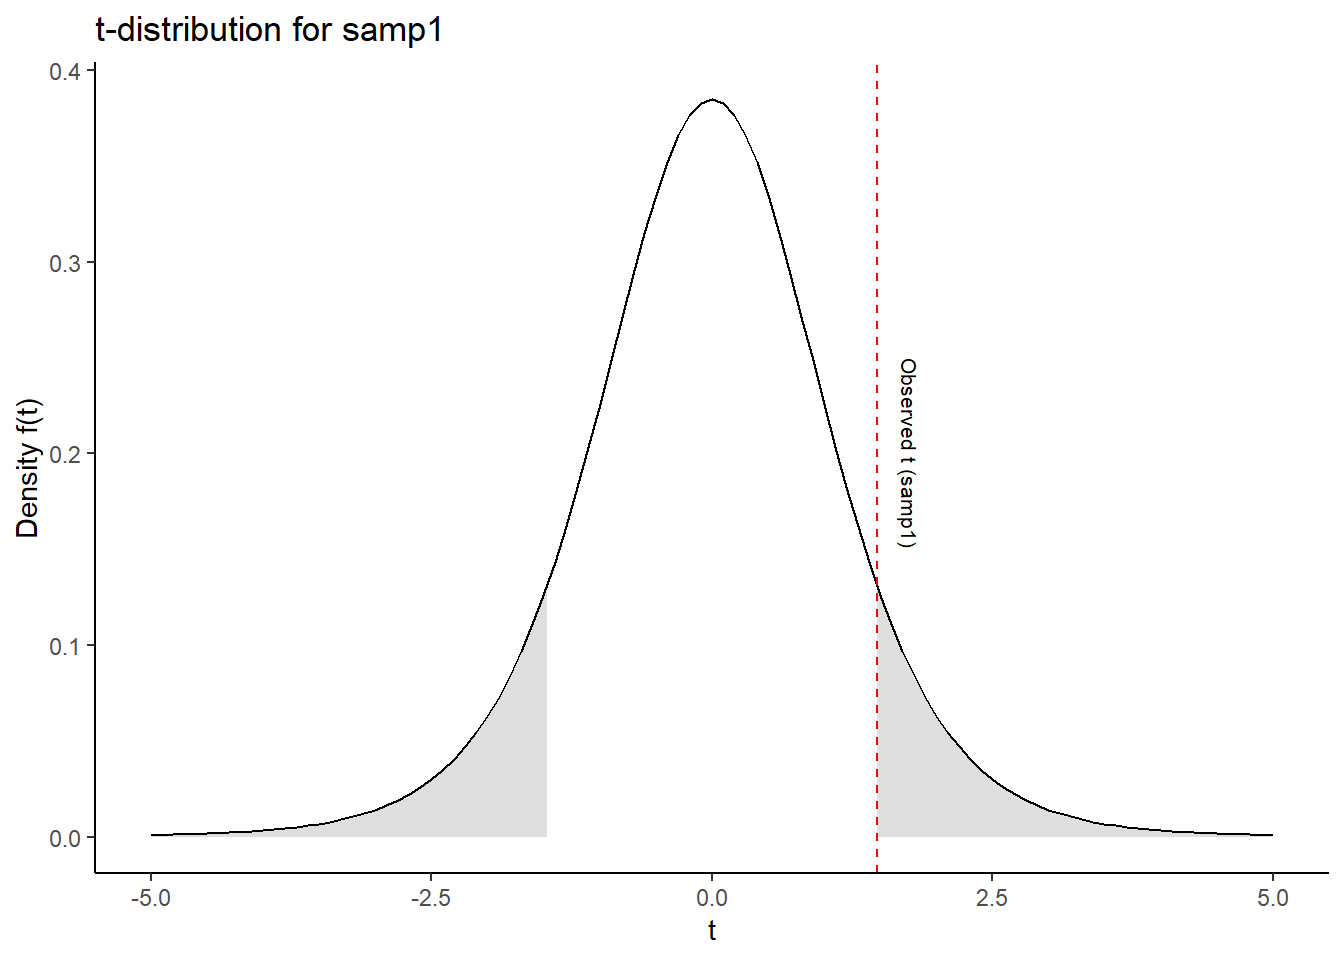
\includegraphics[keepaspectratio]{03-statistical-inference_files/figure-pdf/fig-samp1-1.pdf}}

}

\caption{\label{fig-samp1}t-fordeling av \texttt{samp1}.}

\end{figure}%

\section{Spørsmål 1 - Forklaring av regresjonsresulateter: Estimat, SE,
t-verdi og
p-verdi}\label{spuxf8rsmuxe5l-1---forklaring-av-regresjonsresulateter-estimat-se-t-verdi-og-p-verdi}

\textbf{Estimate}: Den estimerte koeffisienten representerer i
regresjonsanalyser med to variabler hvor mykje vi kan forvente at den
avhengige variabelen endrer seg per endring i den uavhengie variabelen
(Spiegelhalter (2019), s.275). I våre ``intercept-only'' modeller, vil
\emph{estimate} derimot korrespondere til gjennomsnittet av alle
verdiene i de ulike utvalgene, og gi oss et estimat på gjennomsnittet
til populasjonen.

I \texttt{samp1} er utvalgets gjennomsnitt 1.84 noe som er litt ifra
populasjonens faktiske gjennomsnitt på 1.5. Når vi øker størrelsen på
utvalget, slik som i \texttt{samp2}, ser vi at gjennomsnittet nærmer seg
populasjonen: samp2 = 1.564 vs \(\mu\) = 1.5.

\textbf{Standardfeil (SE)}: Standardfeilen måler hvor mykje
\emph{estimate} forventes å variere fra utvalg til utvalg (Spiegelhalter
(2019), s.231, 403-404). Standardfeilen sier dermed hvor mye
gjennomsnittet vil kunne variere fra utvalg til utvalg grunnet tilfeldig
variasjon i dataene. For eksempel sier standardfeilen i \texttt{m2} at
gjennomsnittet vil variere med 0.4774117 for hvert utvalg. SE beregnes
slik:

\[
\text{SE} = \frac{s}{\sqrt{n}}
\]

hvor:

\begin{itemize}
\tightlist
\item
  (s ) er standardavviket til utvalget
\item
  ( n ) er antall observasjoner
\end{itemize}

\textbf{t-verdi}: \emph{t}-verdien, eller \emph{t}-statistikk, beregnes
som \(t = \frac{\text{estimate}}{\text{standard error}}\), og kan
forstås som hvor mange standardfeil estimatet er fra 0 (Spiegelhalter
(2019), s.276-277). Den vil hjelpe oss med å avgjøre om det er fornuftig
å anta at vårt gjennomsnitt er forskjellig fra 0, og om null-hypotesen
burde forkastes eller godtas (Spiegelhalter (2019), s.276-277). Dess
høgere t-verdien er, dess sikrere kan vi være på at estimatet vårt, her
\emph{y}, oppsto ved tilfeldig variasjon gitt at nullhypotesen var sann.

\textbf{p-verdi}: Gitt at vi veit \emph{t}-verdien og størrelsen på
utvalget, kan vi benytte oss av R til å regne ut \emph{p}-verdien, (se
\texttt{summary()} eller \texttt{p1}/\texttt{p2} i koden over):
henholdsvis 0.185 for \texttt{samp1} og 0.002 for \texttt{samp2}.

P-verdi defineres som sannsynligheten for å få et resultat så ekstremt
som det observert, viss null hypotesen er virkelig sann (Spiegelhalter
(2019), s. 264). Hva terskel man setter for p-verdien vil variere basert
på type studie og ønsket effekt, men historisk sett så er den
p\textless0.05 sett på som statistisk signifikant. I vårt tilfelle er
det kun \texttt{m2} som gir oss en p-verdi under 0.05, og er da
statistisk signifikant. Samtidig er det viktig å understreke at
p-verdien ikke sier noe om sannheten til en hypotese eller at statistisk
signifikans betyr at det har praktisk eller klinisk betydning
(Spiegelhalter (2019), s.297-303).

\section{\texorpdfstring{Spørsmål 2 - Årsaker til forskjeller mellom
studieresulatene i modellene \texttt{m1} og
\texttt{m2}.}{Spørsmål 2 - Årsaker til forskjeller mellom studieresulatene i modellene m1 og m2.}}\label{spuxf8rsmuxe5l-2---uxe5rsaker-til-forskjeller-mellom-studieresulatene-i-modellene-m1-og-m2.}

Det første som burde påpekes er ulik utvalgsstørrelse på de to
modellene. Ved større utvalg blir estimatene gjerne mer presise fordi
tilfeldige variasjoner glattes ut. For eksempel så vil standardfeilen
bli påvirket av størrelsen på utvalget, ved at et større utvalg vil føre
til en lavere standardfeil (ref formelen over), som igjen kan gi en mer
signifikant t-verdi og lavere p-verdi. Dette er tilfelle i modellene
våre over, der \texttt{m2} har et større utvalg som fører til en lavere
standardfeil, mer signifikant t-verdi og lavere p-verdi sammenlignet med
\texttt{m1} (Spiegelhalter (2019), s.191-192).

Den lave utvalgsstørrelsen i \texttt{m1} vil også føre til at tilfeldige
variasjoner i datane vil kunne føre til at resultatene avviker mer fra
den sanne populasjonsgjennomsnittet enn \texttt{m2}. Forskjellen i
standardfeilen mellom de to modellene, sier at det er forskjellig
spredning i observasjonene. Den økte spredningen i \texttt{m1} vil bidra
til mindre presise estimater, høyere p-verdi og mindre signifikante
resultater (Spiegelhalter (2019), s.195).

\section{\texorpdfstring{Spørsmål 3 - Betydningen av skyggeområdene i
halområdene til t-fordelingen i
Figure~\ref{fig-samp1}.}{Spørsmål 3 - Betydningen av skyggeområdene i halområdene til t-fordelingen i Figure~.}}\label{spuxf8rsmuxe5l-3---betydningen-av-skyggeomruxe5dene-i-halomruxe5dene-til-t-fordelingen-i-fig-samp1.}

De skyggelagte områdene hjelper å visualisere hvor sannsynlig eller
usannsynlig den observerte t-verdien, gitt at nullhypotesen er sann
(dvs. at \(\mu\) = 1.5). Ved å skyggelegge begge halene visualiseres man
sannsynligheten for å få en t-verdi enten på den positive eller negative
siden. Dess mindre det skyggelagte området er, desto mindre er det at vi
vil observere en så ekstrem t-verdi, og desto mer sannsynlig er det at
vi kan forkaste nullhypotesen.

\bookmarksetup{startatroot}

\chapter{Simulering til spørsmål
4-7}\label{simulering-til-spuxf8rsmuxe5l-4-7}

Under er en kode som lagrer resultatet fra 1000 utførte studier, for å
kunne utvikle en faktisk utvalgsdistribusjon. Ved å bruke
\texttt{results} datasettet, skal eg svare på spørsmålene 4-7.

\section{Spørsmål 4 - Sammenligning av standardavvik og SE for
utvalgsstørrelser (n = 8 og n = 40): Forklaring og
definisjon.}\label{spuxf8rsmuxe5l-4---sammenligning-av-standardavvik-og-se-for-utvalgsstuxf8rrelser-n-8-og-n-40-forklaring-og-definisjon.}

I Table~\ref{tbl-summary} er det en oppsummering av standardavviket til
\texttt{estimate} og gjennomsnittet av \texttt{se}:

\begin{longtable}[]{@{}rrr@{}}

\caption{\label{tbl-summary}Oppsummerende statistikk for standardavviket
til \texttt{estimate} og gjennomsnittet av \texttt{se}.}

\tabularnewline

\toprule\noalign{}
Utvalgsstørrelse & Standardavvik & SE \\
\midrule\noalign{}
\endhead
\bottomrule\noalign{}
\endlastfoot
8 & 1.0708432 & 1.0213745 \\
40 & 0.4838475 & 0.4696954 \\

\end{longtable}

Standardavviket av estimatene vil fortelle hvor mye estimatene vil
variere fra prøve til prøve når vi trekker et tilfeldig utvalg av
populasjonen - med andre ord vil det være den naturlige variasjonen i
gjennomsnittet i utvalgene. Standardfeilen, har vi tidligere forklart,
måler hvor mye vi forventer et estimat fra et enkelt utvalg vil avvike
fra det sanne gjennomsnittet av populasjonen. Begge disse målene er
relatert til den variasjonen vil vi kunne se i dataene, og sier oss noe
om usikkerheten rundt gjennomsnittet i utvalget.

Standardfeilen kan på mange måter ses på som et mål for presisjonen på
estimatet (Spiegelhalter (2019), s.231). I vårt tilfelle vil det si hvor
presist utvalgets gjennomsnitt estimerer populasjonens gjennomsnitt.
Dess flere prøver man tar, vil standardfeilen nærme seg standardavviket
av estimatene, fordi begge måler hvor mye estimatene varierer rundt det
sanne gjennomsnittet.

\section{Spørsmål 5 - Histogram av p-verdier og effekten av
utvalgsstørrelse på statistisk
styrke}\label{spuxf8rsmuxe5l-5---histogram-av-p-verdier-og-effekten-av-utvalgsstuxf8rrelse-puxe5-statistisk-styrke}

Figure~\ref{fig-histo} under viser fordelingen av p-verdier for n = 8 og
n = 40, basert på de 1000 prøvene som har blitt generert.

\begin{figure}

\centering{

\pandocbounded{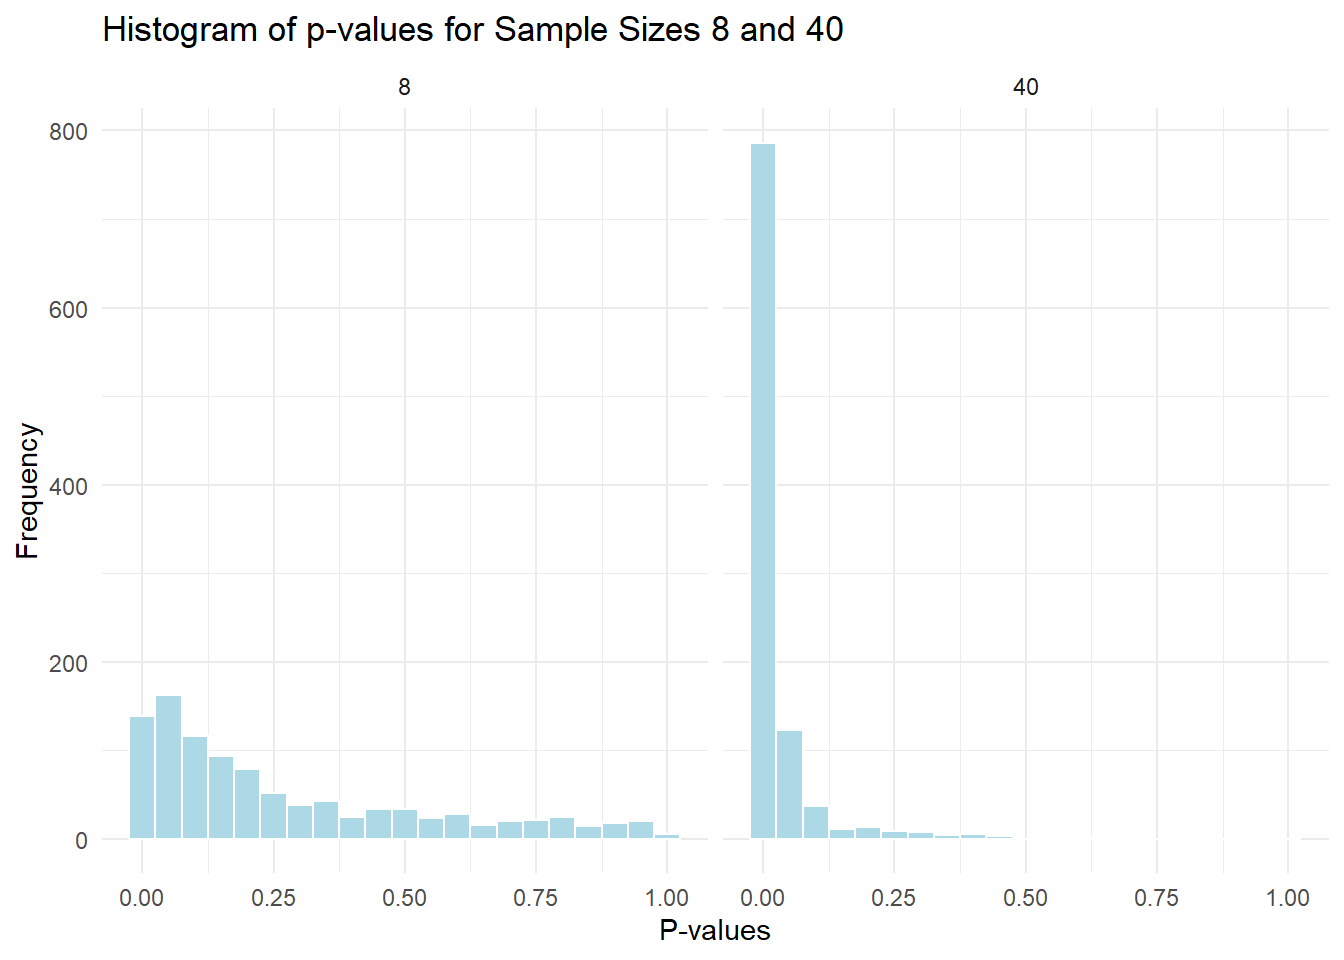
\includegraphics[keepaspectratio]{03-statistical-inference_files/figure-pdf/fig-histo-1.pdf}}

}

\caption{\label{fig-histo}Histogram of p-values for Sample Sizes 8 and
40}

\end{figure}%

Basert på tidligere diskusjon rundt usikkerheten og variasjon rundt
estimatene, vil vi forvente å se en fordeling med flere p-verdier som er
høyere enn 0.05 og dermed ikkje statistisk signifikant for \emph{n = 8}.
Noe som kommer tydelig frem i Figure~\ref{fig-histo}. For \emph{n = 40}
vil vi motsetning forvente at flere p-verdier som er lavere en 0.05, noe
som vi også er tydelig i Figure~\ref{fig-histo}.

\textbf{Statistisk power}, er beskrevet som sannsynligheten for å
oppdage en sann effekt om den er tilstede (Spiegelhalter (2019), s.285).
I praksis kan vi tenke på at høgere statistisk power øker sjansen til å
finne signifikante resulateter når det finnes en reel effekt.

En faktor som vi så fint får visualisert i Figure~\ref{fig-histo}, er at
statistisk power avhenger av blant annet utvalgsstørrelsen. Basert på
det vi observerer i histogrammet, vil vi med større sikkerhet si at vi
står bedre egnet til å oppdage en sann effekt (her det sanne
gjennomsnittet) ved n = 40.

\section{Spørsmål 6 - Antall studier med signifikante effekter for hver
utvalgsstørrelse}\label{spuxf8rsmuxe5l-6---antall-studier-med-signifikante-effekter-for-hver-utvalgsstuxf8rrelse}

For at studiene fra hvert utvalg skal bli med i summeringen, må de ha
eit signifikansnivå på \(\alpha < 0.05\). Under i Table~\ref{tbl-sig}
ser man oversikten av hvor mange studier fra hvert utvalgsmål som er
statistiske signifikante:

\begin{longtable}[t]{rr}

\caption{\label{tbl-sig}Proportion of Significant Results by Sample
Size}

\tabularnewline

\toprule
n & α\\
\midrule
8 & 0.227\\
40 & 0.865\\
\bottomrule

\end{longtable}

\section{\texorpdfstring{Spørsmål 7 - Beregning av statistisk styrke for
en t-test med ulike utvalgsstørrelser ved bruk av
\texttt{pwr}-pakken.}{Spørsmål 7 - Beregning av statistisk styrke for en t-test med ulike utvalgsstørrelser ved bruk av pwr-pakken.}}\label{spuxf8rsmuxe5l-7---beregning-av-statistisk-styrke-for-en-t-test-med-ulike-utvalgsstuxf8rrelser-ved-bruk-av-pwr-pakken.}

I Table~\ref{tbl-pwr} er det vist den statistiske poweren for de ulike
utvalgsstørrelsene. Som det ble nevnt tidligere, vil en høyere power
styrke sannsynlighetene for å finne en signifikant forskjell viss den
eksisterer, f.eks: en statistisk power på 0.8 tilsvarer at det er 80\%
sannsynlighet for at vi vil oppdage en statistisk forskjell viss den
eksisterer.

\begin{longtable}[]{@{}rr@{}}

\caption{\label{tbl-pwr}Statistical Power for Different Sample Sizes}

\tabularnewline

\toprule\noalign{}
Sample.Size & Power \\
\midrule\noalign{}
\endhead
\bottomrule\noalign{}
\endlastfoot
8 & 0.2320770 \\
40 & 0.8693981 \\

\end{longtable}

Den lave styrken for n = 8 sammenlignet med n = 40 som vi ser i
Table~\ref{tbl-pwr}, henger sammen med at det var færre
ikke-signifikante tester for n = 8 versus n = 40 i Table~\ref{tbl-sig}.
Gjennomgående for når vi har sammenlignet de statistiske parametrene
mellom de ulike utvalgene, er at eit større utvalg har gitt meir
presisjon. Dette samsvarer godt med den statistiske poweren også: større
utvalg vil øke sannsynligheten for signifikante resultater og økt
statistisk power.

\section{Spørsmål 8 - Antall falske positive resultater ved 5 \%
signifikansnivå ved gjentatte
studier.}\label{spuxf8rsmuxe5l-8---antall-falske-positive-resultater-ved-5-signifikansnivuxe5-ved-gjentatte-studier.}

I koden under har eg laget et nytt datasett med resultater fra flere
tilfeldige utvalg med n = 8 og n = 40, fra en populasjon med en
gjennomsnittlig effekt på 0.

Videre har eg laget et histogram, Figure~\ref{fig-histo0}, for å
visualisere andelen av p-verdier for de forskjellige utvalgsstørrelsene.

\begin{figure}

\centering{

\pandocbounded{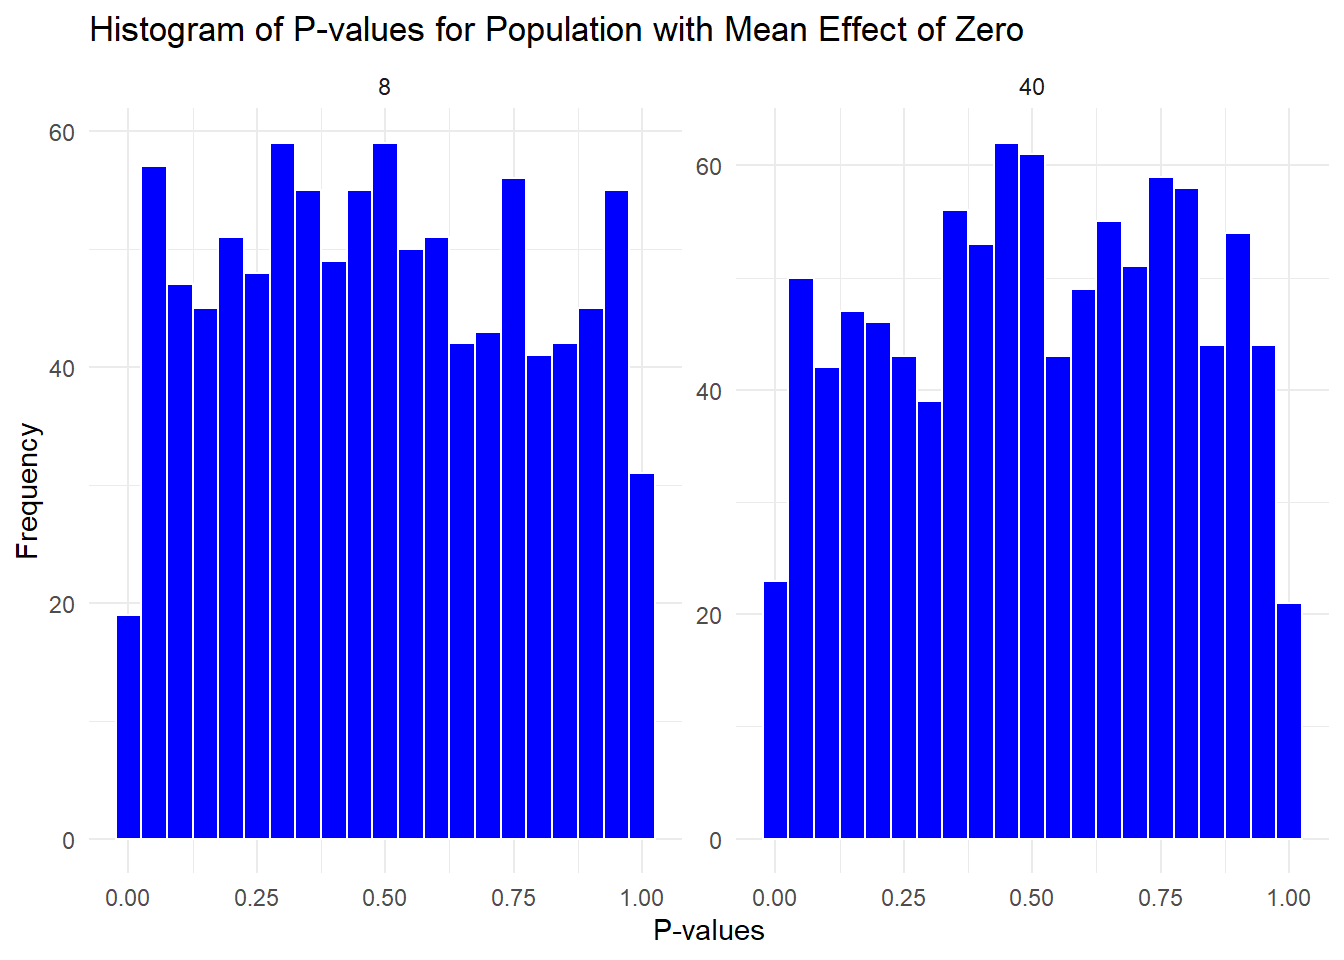
\includegraphics[keepaspectratio]{03-statistical-inference_files/figure-pdf/fig-histo0-1.pdf}}

}

\caption{\label{fig-histo0}Histogram of P-values for Population with
Mean Effect of Zero}

\end{figure}%

Et ``falskt positivt'' resultat oppstår når p-verdien er mindre enn
signifikansnivået (her \(\alpha < 0.05\)), selv om den sanne effekten i
populasjonen er null (Spiegelhalter (2019), s.278). I
Table~\ref{tbl-falsk} ser vi at selv om effekten på populasjonen er lik
null, er det omtrent 5\% av studiene for begge utvalgsstørrelsene som
feilaktig viser en statistisk signifikant effekt. Dette demonstrer i
praksis konseptet med et signifikansnivå (\(\alpha < 0.05\)), som betyr
at vi tillater en 5\% sjanse for å forkaste nullhypotesen når den er
sann, bedre kjent som type I feil (Spiegelhalter (2019), s.283).

\begin{longtable}[]{@{}
  >{\raggedleft\arraybackslash}p{(\linewidth - 6\tabcolsep) * \real{0.0423}}
  >{\raggedleft\arraybackslash}p{(\linewidth - 6\tabcolsep) * \real{0.3239}}
  >{\raggedleft\arraybackslash}p{(\linewidth - 6\tabcolsep) * \real{0.2817}}
  >{\raggedleft\arraybackslash}p{(\linewidth - 6\tabcolsep) * \real{0.3521}}@{}}

\caption{\label{tbl-falsk}Resultater av falske positive og
ikke-signifikante tester per utvalgsstørrelse}

\tabularnewline

\caption{Resultater av falske positive og ikke-signifikante tester per
utvalgsstørrelse}\tabularnewline
\toprule\noalign{}
\begin{minipage}[b]{\linewidth}\raggedleft
n
\end{minipage} & \begin{minipage}[b]{\linewidth}\raggedleft
Antall falske positive
\end{minipage} & \begin{minipage}[b]{\linewidth}\raggedleft
Falske positive (\%)
\end{minipage} & \begin{minipage}[b]{\linewidth}\raggedleft
Antall ikke-signifikante
\end{minipage} \\
\midrule\noalign{}
\endfirsthead
\toprule\noalign{}
\begin{minipage}[b]{\linewidth}\raggedleft
n
\end{minipage} & \begin{minipage}[b]{\linewidth}\raggedleft
Antall falske positive
\end{minipage} & \begin{minipage}[b]{\linewidth}\raggedleft
Falske positive (\%)
\end{minipage} & \begin{minipage}[b]{\linewidth}\raggedleft
Antall ikke-signifikante
\end{minipage} \\
\midrule\noalign{}
\endhead
\bottomrule\noalign{}
\endlastfoot
8 & 44 & 4.4 & 956 \\
40 & 49 & 4.9 & 951 \\

\end{longtable}

\bookmarksetup{startatroot}

\chapter{Vedlegg: Koder brukt}\label{vedlegg-koder-brukt}

Her vises alle kodene som er blitt brukt:

Tabell ``Oversikt over de parametrene som vil bli diskutert videre i
oppgaven.''

\begin{table}
\caption*{
{\large Parametere for modellene m1 og m2}
} 
\fontsize{12.0pt}{14.4pt}\selectfont
\begin{tabular*}{\linewidth}{@{\extracolsep{\fill}}lrr}
\toprule
Parameter & m1 & m2 \\ 
\midrule\addlinespace[2.5pt]
Estimat & 1.8397275 & 1.564160975 \\ 
Standardfeil & 1.2512930 & 0.477411701 \\ 
t-verdi & 1.4702611 & 3.276335647 \\ 
p-verdi & 0.1849546 & 0.002212965 \\ 
\bottomrule
\end{tabular*}
\end{table}

\bookmarksetup{startatroot}

\chapter{Assignment 4: Study design}\label{assignment-4-study-design}

\bookmarksetup{startatroot}

\chapter{Innledning}\label{innledning}

Tradisjonelt sett er plyometrisk trening den vanligste treningsmetoden
for å forbedre en persons evne til rask kraftutvikling, og er derfor
ofte brukt innen sprint- og hoppidretter ((\textbf{Markovic2007?})).
Selv om evnen til rask kraftutvikling er viktig for prestasjon, er
utvikling av maksimal kraft også viktig. Et individs evne til å
produsere impuls, som er et produkt av rate of force development (RFD)
og maksimal kraft, er en avgjørende egenskapen for prestasjon i
eksplosive og kraftfulle idretter ((\textbf{cleather2021?}), s.20-22).
For å bedre forstå hvordan plyometrisk trening påvirker prestasjon i
slike idretter, har jeg valgt ut fem studier som ser nærmere på effekten
av plyometrisk trening på kraftutvikling.

De fem inkluderte studiene vil bli analysert ved hjelp av QALMRI-metoden
(``Question'', ``Alternatives'', ``Methods'', ``Results'' og
``Inferences''), en evidensbasert tilnærming som sikrer en grudig
forståelse av nøkkelpunktene og kritisk vurdering av empiriske artikler
((\textbf{Brosowsky2020?})). I stedet for å gi en detaljert gjennomgang
av hver enkelt studie, vil jeg vektlegge og sammenligne studienes design
og valg av statistiske analyser som er brukt for å besvare
forskningsspørsmålene. Til slutt vil jeg komme med min anbefaling for
hvordan fremtidige studier kan designes for best mulig å undersøke
effekten av plyometrisk trening på muskelstyrke.

\bookmarksetup{startatroot}

\chapter{Analyse}\label{analyse}

\section{Problemstilling og
hypoteser}\label{problemstilling-og-hypoteser}

De utvalgte studiene har som overordnet mål å undersøke hvordan
plyometrisk trening påvirker sentrale aspekter av fysisk prestasjon,
inkludert maksimal styrke, eksplosivitet og muskeltykkelse, som er
avgjørende i eksplosive og kraftfulle idretter. Hver studie adresserer
hver sin spesifikke problemstilling knyttet til dette målet. Fatourus et
al.~(2000) ønsker å sammenligne effekten ploymetrisk trening,
tradisjonell styrketrening og kombinasjonstrening har på vertikal hopp
prestasjon ((\textbf{Fatouros2000?})). Vissing et al.~(2008) undersøker
hvilke adaptive endringene i maksimal styrke og power som skjer som
følge av enten tradisjonell styrketrening eller plyometrisk
styrketrening ((\textbf{Vissing2008?})). McKinlay et al.~(2018)
adresserer hvordan plyometrisk trening påvirker nevromuskulære
funksjoner og muskulære tilpasninger hos unge fotballutøvere
((\textbf{McKinlay2018?})). Whitehead et al.~(2018) fokuserer på
kortsiktige effekter av plyometrisk og styrketrening på muskelstyrke og
eksplosiv prestasjon ((\textbf{Whitehead2018?})). Mens Harput et
al.~(2023) utforsker effekten av plyometrisk trening på hoppytelse,
muskeltykkelse og muskelstyrke i quadriceps hos unge kvinnlige
volleyballspillere ((\textbf{Harput2023?})).

Ingen av studiene definerer et klart forskningsspørsmål knytt til
problemstillingen sin. De fleste av de aktuelle studiene presenterer en
klar hypotese om at plyometrisk trening vil gi lik eller bedre
resultater i eksplosivitet, muskelstyrke eller nevromuskulære
tilpasninger sammenlignet med andre treningsmetoder, som Harput et
al.~(2023), Vissing et al.~(2008), McKinlay et al.~(2018) og Whitehead
et al.~(2018)
((\textbf{McKinlay2018?});(\textbf{Harput2023?});(\textbf{Vissing2008?});(\textbf{Whitehead2018?})).
Fatouros et al.~(2000) derimot, beskriver heller formålet med studien
uten å formulere et forskningsspørsmål eller en hypotese
((\textbf{Fatouros2000?})). Tngsmetodene.

Hypotesene i studiene deler en antakelse om at plyometrisk trening vil
kunne forbedre muskelens evne til å generere kraft hurtig, altså power
((\textbf{Raastad2010?}), s.225). Det finnes imidlertid flere
alternative forklaringer på resultatene som kan påvirke dataene. En
mulig årsak kan være at intensiteten i den plyometriske treningen var
høyere enn kontrolltreningen, noe som førte til forbedringer uavhengig
av treningsmetode ((\textbf{Raastad2010?}), s.231-233). Deltagernes
treningsbakgrunn kan også påvirke responesen på treningen, i tillegg til
faktorer som dagsformen på testdagen, som kan bidra til ytterligere
variasjon i prestasjonene. Det er også mulig at forbedringene i
eksplosivitet skyldes nevromuskulære tilpasninger enn spesifikke
effekter av plyometrisk trening ((\textbf{Raastad2010?}), s.64). Videre
kan placeboeffekten spille en rolle, da forbedringene kan være påvirket
av deltakernes forventninger om framgang ved å delta i et
treningsopplegg.

Plyometrisk trening beskrives som en sentral metode for å forbedre
prestasjon der det stilles krav til hurtig kraftutvikling, og antas å
kunne gi lignende eller bedre muskulære og nevromuskulære tilpasninger
sammenlignet med tradisjonell styrketrening ((\textbf{Whitehead2018?}),
s.2743-2744;(\textbf{markovic2010?})). Samtidig påpekes det at det
finnes begrenset forskning på hvorfor plyometrisk trening forbedrer
prestasjon, og hvilke spesifikke tilpasninger som ligger bak disse
forbedringene ((\textbf{McKinlay2018?}),
s.3039-3040;(\textbf{Harput2023?}), s.89;(\textbf{Vissing2008?}),
s.1800;(\textbf{Fatouros2000?}), s.471). Basert på disse
kunnskapshullene har forfatterne av de utvalgte studiene formulert
hypoteser om at plyometrisk trening vil kunne gi lik eller større
forbedring i prestasjon i bevegelser som krever rask kraftutvikling,
sammenlignet med tradisjonell styrketrening, og samtidig undersøke
hvilke underliggende mekanisker som fører til disse tilpasningene.

\section{Metode}\label{metode-4}

\subsection{Valg av studiedesign}\label{valg-av-studiedesign}

Valg av studiedesign er avgjørende for å kunne svare på
forskningsspørsmålet eller teste hypoteser.Studiedesignet strukturerer
studien på en måte som gjør det mulig å trekke holdbare slutninger
((\textbf{browner2022?}), s.3). Valget av design avhenger blant annet om
man planlegger å igangsette en intervensjon for å undersøke dens
effekter. Slike studier, kjent som analytiske studier, prøver å evaluere
sammenhenger og trekke slutninger om årsak-virkning-forholdet
((\textbf{browner2022?}), s.5). En typisk analytisk studiedesign er en
randomisert kontrollert studie (RCT). Før man gjennomfører en slik
studie, er det vanlig at deskriptive studier har blitt utført for å
undersøke karakteristikker ved en populasjonen, som for eksempel
muskelmasse hos eliteutøvere ((\textbf{browner2022?}), s.4). En tydelig
beskrivelse av studiedesignet og begrunnelse av valget er avgjørende for
å gi leserne instinkt i forskerens vurderinger.

Som nevnt tidligere, er det overordnet målet med de utvalgte studiene å
undersøke hvordan plyometrisk trening påvirker fysisk prestasjon,
inkludert maksimal styrke, eksplosivitet og muskelmasse. Fire av
studiene har valgt å tilfeldig fordele deltakerne til enten å
gjennomføre trening (intervensjon) eller ikke (kontroll)
((\textbf{Fatouros2000?});(\textbf{McKinlay2018?});(\textbf{Vissing2008?});(\textbf{Whitehead2018?})),
slik det gjøres i en RCT-studie. Den femte studien valgte imidlertid et
prospektivt kohortdesign, der deltakerne ble fulgt opp over tid uten
randomisering ((\textbf{Harput2023?})).Ved å randomisere deltagerne
mellom gruppene i RCT-studiene minimeres påvirkningen av konfunderende
variabler som kan forstyrre resultatene, mens kohortstudier gir
mulioghet til å observere naturlige endringer i en populasjon over tid
uten intervensjon i gruppefordelingen ((\textbf{browner2022?}), s.4, 6,
116, 196).

I RCT-studiene som Fatouros et al.~(2000), McKinlay et al.~(2018),
Vissing et al.~(2008) og Whitehead et al.(2018) gjennomførte, vil valget
om randomisering bidra til å redusere risikoen for at andre faktorer enn
treningen selv påvirket resultatene, som treningsbakgrunn, noe som vil
styrke validiteten av konklusjonene om årsakssammenheng mellom
intervensjon og fysisk prestasjon. Ingen av studiene benyttet derimot
blinding i sitt design, noe som kan ha introdusert rapporteringsbias,
særlig siden både deltakerne og forskerne visste hvilken gruppe
deltakerne tilhørte ((\textbf{browner2022?}), s.196, 397). Dette er ikke
noe nytt for treningsintervensjoner, der det er praktisk vanskelig å
skjule gruppetilhørlighet.

I kohortstudien av Harput et al.~(2023), var det derimot ikke mulig å
bruke randomisering. Forskerne fulgte deltakerne over tid for å
observere endringer etter en allerede igangsatt treningsintervensjon,
noe som tillot forskerne å se naturlige variasjoner i prestasjonene uten
inngrep i gruppefordelingen ((\textbf{browner2022?}) s.4, 116). Samtidig
gjør dette at kohortstudier er mer utsatt for konfunderende variabler,
siden deltakerne ikke blir tilfeldig fordelt i grupper. Dette kan
påvirke validiteten i forhold til årsakassammenhenger, men samtidig er
slike design mer gjennomførbar for å undersøke langtidseffekter i en
realistisk setting.

\subsection{Utvalg}\label{utvalg}

Ingen av studiene definerer eller beskriver en bestemt populasjon i
detalj, og det er varierende grad av informasjon om deltakerne. Generelt
tar studiene for seg unge, aktive idrettsutøvere eller utrente
menn/ungdommer, men ikke alle går i dybden på demografiske faktorer som
kan påvirke generaliserbarheten av resultatene ((\textbf{browner2022?}),
s.26-27). For eksempel bestod utvalget i Vissing et al.~(2008) av en
relativt homogen gruppe med utrente menn, mens Harput et al.~(2023)
fokuserte på en mer spesifikk, men potensielt heterogen gruppe av unge
volleyballspillere ((\textbf{Vissing2008?});(\textbf{Harput2023?})).
Selv om informasjon om gruppene kan være mangelfull, ser de fleste
studiene ut til å ha relativt homogene utvalg med hensyn til
treningsstatus og idrettsbakgrunn.

Det er blitt brukt varierende metoder for å rekruttere deltakere i
studiene, og graden av detaljer informasjon om rekruttering og
begrunnelse for utvalgsstørrelse varierer. Både Vissing et al.~(2008) og
Fatouros et al.~(2000) rekrutterte frivillige
((\textbf{Fatouros2000?});(\textbf{Vissing2008?})), mens Harput et
al.~(2023) brukte en kohort av volleyballspillere
((\textbf{Harput2023?})). De to siste studiene gir derimot lite
informasjon om rekrutteringsprosessen, men det kan virke som deltagerne
er rekruttert fra lokale ungdomslag.

Kun Vissing et al.~(2008) rapporterte en power-beregning for å sikre
tilstrekkelig statistisk styrke (0.8), mens de andre ikke oppga dette
((\textbf{Vissing2008?}), s.1830). Power referer til sannsynligheten for
å oppdage en statistisk signifikant forskjell i utfall mellom gruppene,
gitt at det eksisterer en slik forskjell ((\textbf{browner2022?}), s.6).
En power-beregning beregner hvor mange deltakere som trengs i hver
gruppe av studien for å ha en viss sannsynlighet for å finne en
signifikant forskjell dersom den finnes ((\textbf{browner2022?}), s.6)
Når Vissing et al.~(2008) oppgir en power på 0.8, betyr det at de med
80\% sannsynlighet vil kunne oppdage en forskjell dersom den eksisterer.
Mangel på power-beregning i de andre studiene kan svekke deres evne til
å trekke pålitelige konklusjoner.

\subsection{Tester og sentrale
variabler}\label{tester-og-sentrale-variabler}

I de inkluderte studiene ble ulike tester gjennomført før og etter
treningsintervensjonene for å måle endringer i fysisk prestasjon,
muskelstyrke og eksplosivitet. Harput et al.~(2023) benyttet
isokinetiske styrkemålinger og ultralyd for å vurdere muskeltykkelse,
styrke og hopphøyde før og etter en seks ukers periode med plyometrisk
trening ((\textbf{Harput2023?})). Vissing et al.~(2008) og McKinlay et
al.~(2018) brukte på sin side dynamiske tester som vertikale hopp og
sprint før og etter treningsperioden
((\textbf{McKinlay2018?});(\textbf{Vissing2008?})). Selv om alle
studiene hadde som mål å undersøke effekten av plyometrisk trening,
varierer testdesignene avhengig av spesifikke forskningsspørsmål eller
hypoteser. Dette fører til ulike valg av variabler som hopphøyde,
muskelstyrke og eksplosivitet, som alle er sentrale faktorer for
prestasjon i kraftbaserte idretter. Valget av disse variablene
reflekterer hver studies formål og hypotese, og illusterer variasjonene
i design og metodevalg mellom studiene.

\subsection{Statistiske tester}\label{statistiske-tester}

Som tidligere nevnt, har de inkluderte studiene som mål å undersøke
hvordan plyometrisk trening påvirker viktige utfallsmål på fysisk
prestasjon, som muskelstyrke og hopphøyde. Selv om studiene benytter
ulike studiedesign og variabler, tilpasset sitt spesifikke
forskningsspørsmål eller hypoteser, har de alle til felles at de måler
endringer i sine definerte utfallsmål over tid og mellom
treningsintervensjoner. For å kunne trekke konklusjoner om effekten av
intervensjonene har ale studiene valgt Analysis of Variance (ANOVA) som
sin primære statistiske metode.

ANOVA er en statistisk test som gjør det mulig å sammenligne
gjennomsnittet mellom flere grupper for å avgjøre om variasjonen mellom
gruppene er så stor at det er usannsynlig å anta at det kun skyldes
tilfeldigheter ((\textbf{Diez2022?}), s.322, 326). I denne analysen
beregnes mean square between groups (MSG), som representerer
variabiliteten mellom gruppene. Dette sammenlignes med mean square error
(MSE), som refleterer variasjonene innenfor hver gruppe, og gir et mål
på naturlig variasjon når nullhypotesen er sann ((\textbf{Diez2022?}),
s.326). Forholdet mellom MSG og MSE, utgjør F-statistikken:

\[
F = \frac{MSG}{MSE}
\] En høy F-verdi indikerer at forskjellen mellom gruppene er stor
sammenlignet med variasjonene innad i gruppene, noe som kan tyde på en
signifikant effekt av treningen ((\textbf{Diez2022?}), s.326-327). Det
er viktigå påpeke at for at ANOVA skal gi sterke bevis mot nullhypotesen
om at utvalggjennomsnittene (\(\mu_i\)) er like, må flere forutsetninger
være oppfylt. For det første må observasjonene være uavhengige både
innad og mellom gruppene. Videre må dataene innenfor hver gruppe være
tilnærmet normalfordelt, og variasjonen mellom gruppene er lik
((\textbf{Diez2022?}), s.322).

I de inkluderte studiene ble både en-veis og to-veis ANOVA brukt for å
analysere dataene. En-veis ANOVA sammenligner gjennomsnittene mellom
flere grupper ved å bruke en avhengig variable for å avgjøre om det
finnes en statistisk signifikant forskjell mellom gruppene
((\textbf{Diez2022?}), s.323-325). To-veis ANOVa evaluerer effekten av
to forskjellige faktorer på resultatet, noe som gjør det mulig å
undersøke både hoved- og samspilleffekter mellom de to faktorene
((\textbf{Diez2022?}), s.329-331). For eksempel brukte Whitehead et
al.~(2018) en-veis ANOVA for å sammenligne baseline data mellom gruppene
((\textbf{Whitehead2018?}), s.2746). Harput et al.~(2023) og McKinlay et
al.~(2018) brukte to-veis ANOVA for å undersøke interaksjonen mellom tid
(før og etter intervensjon) og gruppetilhørlighet (treningsintervensjon
versus kontroll) ((\textbf{Harput2023?}),
s.92-93;(\textbf{McKinlay2018?}), s.3046). Mens ANOVA forteller at det
finnes forskjeller mellom gruppene, sier den ikke noe om hvilke grupper
som faktisk skiller seg fra hverandre, noe som gjør det vanskelig å
sammenligne treningsintervensjonene opp mot hverandre. For å
identifisere spesifikke gruppedifferanser når ANOVA viste signifikante
resultater, benyttet flere av studiene post hoc-tester som Bonferroni
((\textbf{spieg2019?}), s.280) med signifikansnivå på \(p \leq 0.05\).
Disse tilleggs analysene tillot en mer detaljert undersøkelse av hvor
forskjellene mellom gruppene oppstod, noe som var avgjørende for å
vurdere treningsinduserteeffekter.

\section{Resultat}\label{resultat-3}

Studiene dokumenterer samlet sett en positiv effekt av plyometrisk
trening på sentrale prestasjonsmål som muskelstyrke, eksplosivitet og
hopphøyde sammenlignet med kontrollgruppene ((\textbf{Fatouros2000?}),
s.474;(\textbf{Harput2023?}), s.93;(\textbf{McKinlay2018?}),
s.3046;(\textbf{Vissing2008?}), s.1804;(\textbf{Whitehead2018?}),
s.2747). For eksempel rapporterte Harput et al.~(2023) signifikante
forbedringer i hopphøyde og quadriceps-styrke etter seks uker med
strukturert plyometrisk trening ((\textbf{Harput2023?}), s.93). Vissing
et al.~(2008) viste at plyometrisk trening førte til målbare økninger i
eksplosiv styrke, inkludert forbedrede resultater i vertikale hopp og
sprinttid ((\textbf{Vissing2008?}), s.1804). På tilsvarende måte
dokumenterte McKinlay et al.~(2018) at regelmessig plyometrisk trening
hos unge fotballspillere førte til en markant forbedring i nevromuskulær
funksjon og styrke ((\textbf{McKinlay2018?}), s.3046).

Fatouros et al.~(2000) fant også at plyometrisk trening kombinert med
styrketrening resulterte i ytterligere forbedringer, sammenlignet med
plyometrisk trening alene ((\textbf{Fatouros2000?}), s.474). Totalt sett
belyser disse funnene forskningsspørsmålene og hypotesene is tudiene, og
dokumenterer målbare forbedringer i prestasjon som et resultat av
plyometrisk trening, både alene og i kombinasjon med andre
treningsformer.

\section{Konklusjonene fra studiene}\label{konklusjonene-fra-studiene}

Hovedfunnene fra studiene viser en signifikant sammenheng mellom
plyometrisk trening og bedring i sentrale prestasjonsmål innen
kraftfulle og eksplosive idretter, da særlig muskelstyrke, hopphøyde og
hopphøyde. Studiene rapporterte målbare forbedringer blant deltakerne
sammenlignet med kontrollgruppene, noe som var et sentralt formål i hver
studie. Fatouros et al.~(2000) fant også ut at en kombinasjon av
plyometrisk trening og styrketrening ga større prestasjonsforbedringer
enn plyometrisk treninge alene, noe som indikerer at sammensatte
treningsformer kan gi ytterligere fordeler sammenlignet med isolerte
plyometriske øvelser ((\textbf{Fatouros2000?}), s.474). Likevel så
understreket Fatouros et al.~(2000), at man skal være forsiktig å trekke
konkrete slutninger, da gruppen som mottok den kombinerte
treningsintervensjon også ble eksponert for et høyere samlet
treningsvolum enn gruppen som kun gjennomførte plyometriske trening
((\textbf{Fatouros2000?}), s.474).

Utvalgene i studiene bestod hovedsaklig av unge, aktive individer,
inkludert utrente menn og ungdomsidrettsutøvere som volleyballspillere
og fotballspillere. Forfatterne bemerket at den observerte effekten kan
være påvirket av spesifikke egenskaper ved utvalget, som alder og
treningsbakgrunn ((\textbf{Harput2023?}),
s.94-95;(\textbf{McKinlay2018?}), s.3048-3049;). Dette indikerer at
resultatene hovedsaklig er relevante for lignende grupper og kanskje
ikke kan overføres til andre grupper, som eldre voksne eller personer
med mer treningserfaring.

\bookmarksetup{startatroot}

\chapter{Anbefaling til fremtidige
studier}\label{anbefaling-til-fremtidige-studier}

Ved å bygge videre på de inkluderte studiene om plyometrisk trening, bør
fremtidige studier fokusere på å optimalisere forskningsdesignet for å
oppnå sterkere og mer generaliserbare konklusjoner. En anbefaling er å
inkludere flere aldersgrupper, treningsnivåer og kjønn. Dette vil gi
bedre innsikt i hvordan plyometrisk trening påvirker ulike populasjoner,
inkludert eldre voksne og personer med mer omfattende treningserfaring.
Videre bør fremtidige studier inkluderer flere målepunkter over tid for
å undersøke de langsiktige effektene av plyometrisk trening.

For å kunne trekke kausale slutninger om effekten av plyometrisk på
ulike populasjoner er RCT-er det foretrukne studiedesign, ettersom de
reduserer påvirkningen av konfunderende faktorer. Selv om blinding er
ideelt, er det vanskelig å få til praktisk i treningsintervensjoner. For
å få innsikt i langsiktige endringer og vedvarende effekter anbefales
prospektive kohortstudier over lengre tid. Kombinasjonen avdisse
designene vil gi et mer helhetlig bilde av både kortsiktige og
langsiktige effekter av plyometrisk trening.

Med tanke på statistiske analyser er variasjonsanalyser velegnede for de
anbefalte studiedesign. I RCT-er der kontroll over baselineforskjeller
er ønskelig, som alder eller treningsbakgrunn, vil \textbf{Analysis of
Covariance (ANCOVA)} være en passende metode. ANCOVA justerer for
varians knyttet til konfunderende faktorer (kovariater, f.eks alder
eller kjønn) for å sikre at treningseffektene kan observeres med større
presisjon ((\textbf{Keselman1998?}), s.373). I prospektive kohortstudier
kan \textbf{mixed effects modeller} være ideelle for å håndtere data med
repeterte målinger og variasjon både mellom og innen individer
((\textbf{Baayen2008?}), s.409-410). Dette vil muliggjøre justeringer
for både individuelle forskjeller og gruppeforskjeller, slik at man får
en dypere forståelse av hvordan treningseffekten utvikler seg over tid.

Ved å kombinere slike statistiske metodene med nøye gjennomtenkte
forskningsdesign kan fremtidige studier gi en mer presis og helhetlig
forståelse av plyometrisk trening sine effekter på fysisk prestasjon i
ulike populasjoner.

\bookmarksetup{startatroot}

\chapter{Assignment 5: Analyzing repeated measured
experiments}\label{assignment-5-analyzing-repeated-measured-experiments}

\bookmarksetup{startatroot}

\chapter{Introduksjon}\label{introduksjon-5}

Treningsadaptasjon er en av de mest grunnleggende søylene i
treningsvitenskapen, som sier at kroppen vår kan tilpasse seg den
belastningen den utsettes for, gitt at den får nok tid til å tilpasse
seg den nye belastningen ((\textbf{bompa2019?}), s. 8). Spesielt
skjelettmuskulaturen har vist seg å være et høgts tilpasningsdyktig vev
som kan endre sin egen arkitektur som respons på en gitt stimuli
((\textbf{coffey2007?})). Resultatene på disse tilpasningene er påvirket
av volumet, intensiteten og frekvensen av treningen, i tillegg vil
tilpasningene avhengig av den spesifikke belastningen kroppen og
muskulaturen utsettes for, for eksempel treningsmetode
((\textbf{bompa2019?}), s.3; (\textbf{Raastad2010?}), s.17;
(\textbf{coffey2007?}); (\textbf{izquierdo2004?})).

Styrketrening har vist seg å være avgjørende, ikke bare for
idrettsprestasjoner ((\textbf{washif2022?})), men også for folkehelse og
redusert dødelighet ((\textbf{ruiz2008?})). Denne treningsformen
omfatter aktiviteter som utvikler eller opprettholder vår evne til å
generer maksimal kraft eller dreiemoment ved en spesifikk hastighet
((\textbf{Raastad2010?}), s.17). Trening for maksimal muskelstyrke, der
målet er å øke den høyeste kraften en muskel kan produsere (målt som en
repetisjon maksimum) ((\textbf{Raastad2010?}), s.13), skiller seg fra
trening med hensikt om muskelvekst (hypertrofi), hvor fokus ligger på å
øke muskelens størrelse ((\textbf{schoenfeld2016?})). Flere studier har
undersøkt hvilket treningsvolum som best stimulerer slike tilpasninger
og har identifisert et dose-respons-forhold, hvor økt treningsvolum er
assosiert med større muskelvekst ((\textbf{currier2023?});
(\textbf{schoenfeld2016?})). Et lignende forhold er også blitt observert
for muskelstyrke ((\textbf{ralston2017?})), selv om det er også
foreslått at et høgt treningsvolum kan bremse utviklingen av maksimal
muskelstyrke ((\textbf{zhang2023?})). Muskelens tverrsnitt er en sentral
faktor å ta med, da et større tverrsnitt vil gi et større potensiale for
kraftutvikling ((\textbf{Raastad2010?}), s.20). Dette understreker
behovet for videre undersøkelser av hvordan treningsvolum påvirker både
muskelhypertrofi og styrkeutvikling, samt i hvilken grad endringer i
muskelmasse er sammenfallende med økninger i styrke.

På bakgrunn av tidligere forskning og den noe usikre
dose-respons-sammenhengen mellom optimal treningsvolum og
muskeltilpasninger, er formålet med denne studien å undersøke hvordan
ulike nivåer av treningsvolum påvirker både muskelvekst og muskelstyrke,
ettersom skjelettmuskulaturen er svært tilpasningsdyktig på den
stimulien den utsettes for. Ved å utforske denne sammenhengen håper man
å kunne bidra med økt innsikt som kan være nyttig ved anbefalinger om
optimalt treningsvolum.

\bookmarksetup{startatroot}

\chapter{Metode}\label{metode-5}

\section{Deltagere og studieoversikt}\label{deltagere-og-studieoversikt}

Totalt ble førti-en menn og kvinner inkludert i studien, der
inklusjonskriterene var at de ikke var røykere og var mellom 18 og 40
år. Klare eksklusjonskriterer som redusert muskelstyrke grunnet
tidligere eller nåværende skader, har hatt mer en en ukentlig
styrketrenings økt de siste 12 månedene fra inklusjonsdato, intoleranse
for lokal bedøvelse, samt bruk av medikamenter som kan påvirke
treningsadaptasjoner. Syv deltakere ble ekskludert fra data analysen,
fordi de ikke hadde gjennomført minimum 85\% av de oppsatte treningene
grunnet årsaker som: ubehag eller smerter i underekstremitetene under
trening (\emph{n = 5}), skade påført utenom studieprotokollen (\emph{n =
1}), eller manglende overholdelse av studiedesignet (\emph{n = 1}). Selv
om ingen av de inkluderte deltakerne utførte mer en 1 ukentlig
styrkeøkt, var det tjue deltakere som rapporterte at de var fysisk
aktive ved inklusjon (median på 2 økter i uken, med en range på 0.5-4).
Alle de inkluderte hadde tidligere treningserfaringer med ulike
idretter, som for eksempel lagidretter, skiskytting etc\ldots).

\begin{longtable}[t]{lllll}

\caption{\label{tbl-antro}Deltakerkarakteristikker}

\tabularnewline

\toprule
\multicolumn{1}{c}{ } & \multicolumn{2}{c}{Kvinne} & \multicolumn{2}{c}{Mann} \\
\cmidrule(l{3pt}r{3pt}){2-3} \cmidrule(l{3pt}r{3pt}){4-5}
 & Ekskludert & Inkludert & Ekskludert & Inkludert\\
\midrule
N & 4 & 18 & 3 & 16\\
Alder & 22.9 (1.6) & 22.0 (1.3) & 24.3 (1.5) & 23.6 (4.1)\\
Vekt & 64.6 (9.7) & 64.4 (10.4) & 88.2 (22.4) & 75.8 (10.7)\\
Stature & 166 (8) & 168 (7) & 189 (5) & 183 (6)\\
\bottomrule

\end{longtable}

Verdiene er presentert som gjennomsnitt og standardavvik (SD).

Deltakerne gjennomgikk en treningsintervensjon med 12 uker styrketrening
for hele kroppen i perioden september til november. For å muliggjøre for
differensiereng av treningsvolum for hver deltaker, ble beinøvelsene
utført unilateralt. Hver deltaker fikk tilfeldig utdelt enten ett sett
eller tre sett til enten høgre eller venstre bein. Deltagerne utførte
dermed begge volumprotokollene. Det ble gjennomført måling av maksimal
styrke ved baseline, under (uke 3,5 og 9) og rett etter intervensjonen,
mens muskeltverrsnitt ble målt før og etter, se
Figure~\ref{fig-trening}.

\begin{figure}

\centering{

\pandocbounded{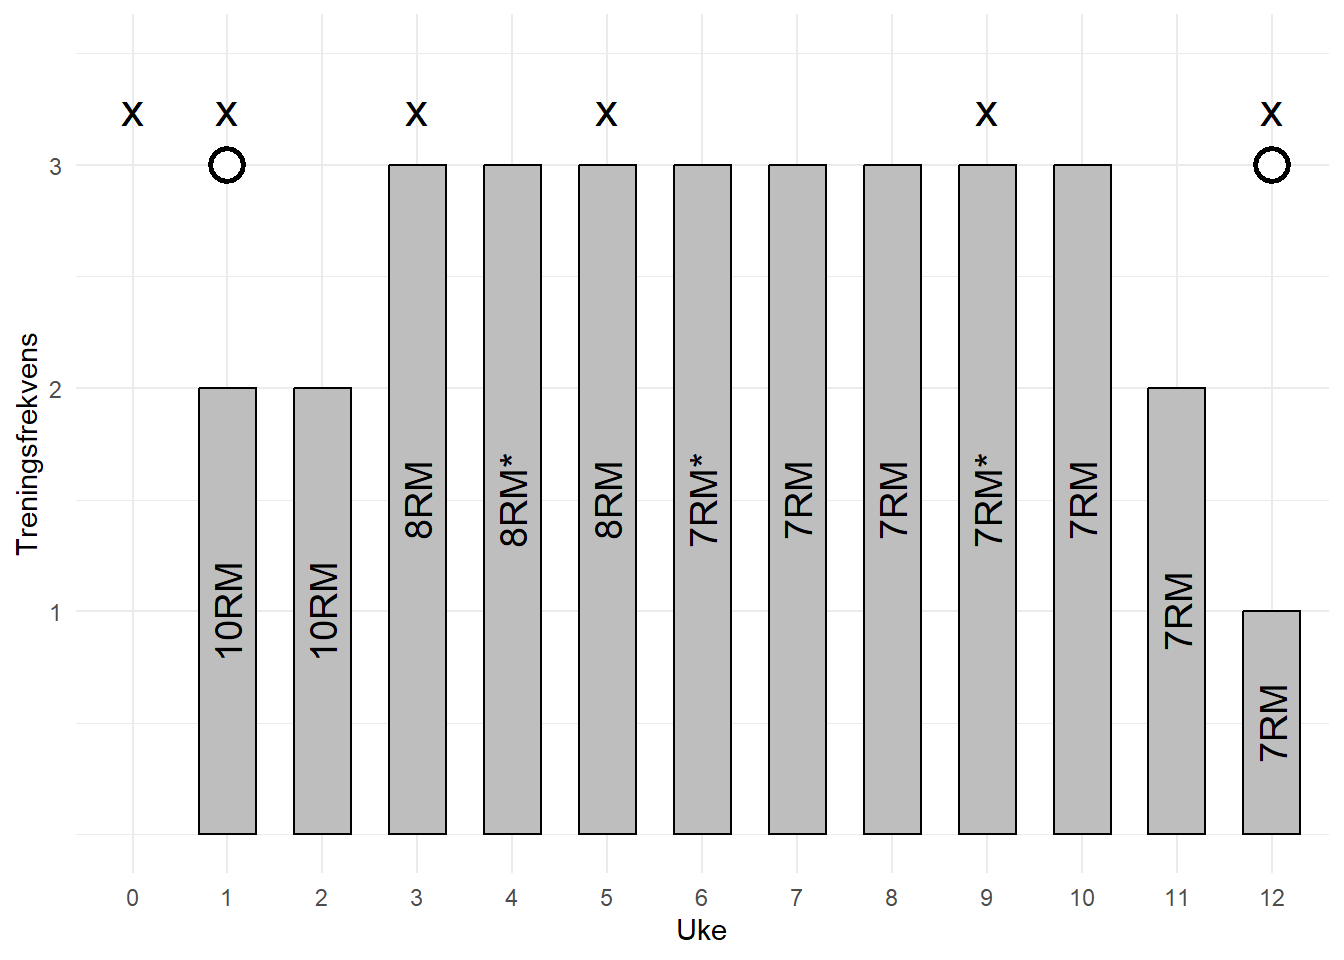
\includegraphics[keepaspectratio]{05-repeated-measurements_files/figure-pdf/fig-trening-1.pdf}}

}

\caption{\label{fig-trening}Studieoversikt}

\end{figure}%

De ulike søylene illustrer treningsfrekvens per uke med en
treningsintensitet lik x repetisjon maksimum (RM). De intensitetne som
er markert med (*), referer til at en av de øktene den uken ble utført
med 90\% av 1RM. Sirkelsymbolet viser til når det ble utført målinger av
muskeltversnitt med hjelp av fullkropps DXA og MR av kneekstensjons
muskelen. X markerer de ulike styrkemålingene: før intervensjonen (n =
34), under (n = 18) og etter (n = 34). Den maksimale styrken før
intervensjonen ble satt som den høgeste verdien deltagerne oppnådde
under to ulike testsekvenser før intervensjonen startet.

\section{Styrketreningsprotokoll}\label{styrketreningsprotokoll}

Det ble laget en standardisert oppvarming som deltakerne skulle
gjennomføre før de begynte med styrketreningen. Oppvarmingen begynte med
5 minutter på ergometer sykkel, der de skulle holde 12-14 på gjennomgått
grad av anstrengelse (RPE). Etter syklingen skulle de gjennomføre 10
repetisjoner av push-ups (tilpasset vanskelighetsgrad basert på vinkel),
sit-ups, knebøy og rygghev, etterfulgt av et sett med 10 repetisjoner av
hver styrkeøvelse med en motstand tilsvarende rundt 50\% av deres
repetisjons maksimum (1RM).

Styrketreningen inneholdt en del for beina og en for overkroppen. For
beina skulle det gjennomføres unilateral beinpress, knefleksjon og
knestrekk, i den nevnte rekkefølgen. Avhengig av gruppen deltakerne ble
tildelt til, ble hver øvelse enten utført med ett sett eller tre sett.
Beinet som ble tildelt ett-setts protokollen gjennomførte arbeidet sitt
mellom det andre og tredje settet til benet som skulle gjennomføre tre
sett. Pausene mellom settene skulle vare mellom 90-180 sekunder. Etter
beinøvelsene hadde blitt fullført, skulle deltakerne gjøre to sett av
bilateral benkpress, nedtrekk og enten skulderpress eller sittende
roinger som ble gjort i hver sin økt. Som man kan se fra
Figure~\ref{fig-trening}, så ble treningsintensiteten gradvis økt fra
10RM to første ukene hadde 10RM, til 8RM de påfølgende tre ukene og 7RM
de siste syv ukene. Etter den niende treningsøkten hadde hver uke som
inneholdt tre økter i uken, en økt med lavere motstand, men der man
beholdt samme antall repetisjoner (motstanden tilsvarte 90\% av økten
før). Øktene med maksimal innsats skulle ikke gjentas før det var gått
48 timer, mens det trengte kun å gå 24 timer mellom ny økt og øktene med
redusert motstand. For å fasiletere til restitusjon, ble det gitt en
standardisert drikk med 0.15 g kg\(^{-1}\) protein, 11.2g kg\(^{-1}\)
karbohydrater og 0.5 g kg\(^{-1}\) fett, etter hver treningsøkt. For å
sikre bærekraftighet av treningsprotokollen, ble det lagt opp til at
noen av øktene kunne gjennomføres uten tilsyn. For å sikre progresjon og
etterlevelse, ble deltakerne instruert til å føre deltaljerte loggbøker
for de øktene som ble utført uten tilsyn, slik at forskerteamet kunne i
samarbeid med deltakerne gå gjennom øktene.

\section{Målinger av maksimal muskelstyrke og muskelens
tverrsnittsareal}\label{muxe5linger-av-maksimal-muskelstyrke-og-muskelens-tverrsnittsareal}

Deltakerne sin maksimale styrke ble satt som deres en repetisjon
maksimum (1RM) i unilateral beinpress og knestrekk. Selve testen
inneholdt en standardisert oppvarming med 10, 6 og 3 repetisjoner på
henholdsvis 50,75 og 85\% av deres antatte repetisjon maksimum. Etter
dette, ble motstanden gradvis økt helt til deltagerne ikke mestret å
løfte vekten gjennom hele bevegelsesbanen, for å finne deres 1RM. Hver
deltaker fikk mellom fire og seks forsøk, der den høgeste vekten de
mestret å løfte i hver øvelse, ble satt som 1RM. Ved baseline, ble 1RM
målt to ganger med minst fire dager mellom hver måling, der den høyeste
i hver test ble brukt i videre analyser. I tillegg til nye målinger
etter endt intervensjon, gjennomførte en del av deltakerne (n = 18)
styrkemålinger underveis i studien (i uke 2, 5 og 9). Det skulle ha gått
minst 48 timer fra forrige treningsøkt før styrketest. De resterende som
ikke utførte tester underveis, ble de ordinære treningsøktene prioritert
ved sykdom eller tidsutfordringer som medførte at de gikk glipp av
trening eller test.

Ved hjelp av magnetisk resonans bildefremstilling (MR), målte man
deltagernes quadricep (vastus lateralis, medialis, intermedius og rectus
femoris) muskeltverrsnittsareal. Dette ble gjort i henhold til
produsentens protokoll (S-Scan, Esaote Europe B.V., Maastricht,
Nederland), og personen som skulle analysere MR-bildene var blindet ved
hjelp av OsiriX (v.5.6, Pixmeo Sarl, Bernex, Sveits). Målingen av
muskeltverrsnittet både før og etter intervensjon, ble gjort på samme
sted på låret, cirka midt på, med samme avstand fra kneleddet.
Resultatet av målingen måtte inneholde minst fire påfølgende bilder med
5 mm tykkelse og 10mm avstand.

\section{Data analyse og statistikk}\label{data-analyse-og-statistikk}

Med mindre noe annet er spesifisert, er alle deskriptive data presentert
som gjennomsnitt og standardavvik. Før studien ble det gjort en
forhåndsberegning av utvalgsstørrelse, som viste at 40 deltakere ville
være tilstrekkelig for å kunne oppdage forskjeller på omtrent 3 og 5
prosentpoeng for henholdsvis muskeltverrsnittsareal og maksimal styrke
mellom de ulike volumforholdene, med en ønsket statistisk styrke på
80\%. Denne beregningen er basert på data fra tidligere studier, som
antar at forskjellene mellom volumforholdene tilsvarer en
effektstørrelse på mellom 0,19 og 0,24 ((\textbf{ralston2017?});
(\textbf{schoenfeld2016?})).

For å undersøke hvordan de ulike volumforholdene påvirket muskelvekst og
styrke, ble det benyttet lineære blandede modeller (LLM). De relative
endringene fra baseline ble satt som den avhengige variabelen, med
antall sett som den uavhengige variabelen. For å vurdere om større
muskelvekst også gir tilsvarende endringer i muskelstyrke, ble en
interaksjonseffekt mellom treningsvolum og endring i muskeltverrsnitt
inkludert. Ved å inkludere denne interaksjonseffekten kan modellen fange
opp eventuelle forskjeller i effekten av muskelvekst på muskelstyrke
under ulike treningsvolum. Baseline-verdier og kjønn ble brukt som
kovariater for å kontrollere for deres potensielle effekt på muskelvekst
og styrke.

For å evaluere om de statistiske modellene oppfylte forutsetningene for
lineære blandede modeller, ble diagnostiske plot undersøkt. Q-Q plot ble
brukt for å vurdere normaliteten til residualene, residualer mot
predikerte verdier for å sjekke for homoskedastisitet, og histogram av
residualer for å identifisere eventuelle skjevheter eller avvik.

Resultater med et signifikansnivå på \(\alpha = 0.05\) ble ansett som
statistisk signifikante. Analysen av dataene ble gjort i R
((\textbf{RCoreTeam2018?})).

\bookmarksetup{startatroot}

\chapter{Resultater}\label{resultater-1}

Under i Table~\ref{tbl-modeller}, er det en oversikt over de sentrale
parametrene for de tre LMM-ene som ble brukt i denne studien.

\begin{table}

\caption{\label{tbl-modeller}Oppsummering av Modellene for Pre og Post}

\centering{

\fontsize{12.0pt}{14.4pt}\selectfont
\begin{tabular*}{\linewidth}{@{\extracolsep{\fill}}llrrrr}
\toprule
Modell & Parameter & Estimert Koeffisient & Standard Feil & t-verdi & p-verdi \\ 
\midrule\addlinespace[2.5pt]
Model 1.1: Leg Extension & (Intercept) & 43.479 & 2.836 & 15.334 & 0.05* \\ 
Model 1.1: Leg Extension & timepost & 33.089 & 1.539 & 21.499 & 0.05* \\ 
Model 1.1: Leg Extension & timepost:setssingle & -4.278 & 2.188 & -1.956 & 0.0513 \\ 
Model 1.2: Leg Press & (Intercept) & 138.164 & 12.091 & 11.427 & 0.05* \\ 
Model 1.2: Leg Press & timepost & 95.326 & 4.158 & 22.926 & 0.05* \\ 
Model 1.2: Leg Press & timepost:setssingle & -8.541 & 5.865 & -1.456 & 0.1462 \\ 
Model 2: Muskel Tverrsnitt & (Intercept) & 7,126.800 & 254.701 & 27.981 & 0.05* \\ 
Model 2: Muskel Tverrsnitt & timepost & 289.876 & 55.046 & 5.266 & 0.05* \\ 
Model 2: Muskel Tverrsnitt & timepost:setssingle & -118.167 & 77.375 & -1.527 & 0.1294 \\ 
\bottomrule
\end{tabular*}

}

\end{table}%

\section{Endring i muskelstyrke}\label{endring-i-muskelstyrke}

\begin{Shaded}
\begin{Highlighting}[]
\CommentTok{\# Last inn dataene}
\FunctionTok{library}\NormalTok{(exscidata)}
\FunctionTok{library}\NormalTok{(tidyverse)}
\FunctionTok{library}\NormalTok{(nlme)}
\FunctionTok{data}\NormalTok{(}\StringTok{"dxadata"}\NormalTok{)}

\CommentTok{\# Filtrer datasettet for leg press{-}øvelsen og sett \textquotesingle{}time\textquotesingle{} som en faktor med ønsket rekkefølge}
\NormalTok{strengthvolume\_legpress }\OtherTok{\textless{}{-}}\NormalTok{ strengthvolume }\SpecialCharTok{\%\textgreater{}\%}
  \FunctionTok{filter}\NormalTok{(exercise }\SpecialCharTok{==} \StringTok{"legpress"}\NormalTok{) }\SpecialCharTok{\%\textgreater{}\%}
  \FunctionTok{mutate}\NormalTok{(}\AttributeTok{time =} \FunctionTok{factor}\NormalTok{(time, }\AttributeTok{levels =} \FunctionTok{c}\NormalTok{(}\StringTok{"pre"}\NormalTok{, }\StringTok{"session1"}\NormalTok{, }\StringTok{"week2"}\NormalTok{, }\StringTok{"week5"}\NormalTok{, }\StringTok{"week9"}\NormalTok{, }\StringTok{"post"}\NormalTok{)))}

\CommentTok{\# Modell for muskelstyrke i legpress{-}øvelsen uten manglende verdier}
\NormalTok{model\_legpress }\OtherTok{\textless{}{-}} \FunctionTok{lme}\NormalTok{(}
  \AttributeTok{fixed =}\NormalTok{ load }\SpecialCharTok{\textasciitilde{}}\NormalTok{ time }\SpecialCharTok{*}\NormalTok{ sets }\SpecialCharTok{+}\NormalTok{ sex,}
  \AttributeTok{random =} \SpecialCharTok{\textasciitilde{}} \DecValTok{1} \SpecialCharTok{|}\NormalTok{ participant,}
  \AttributeTok{data =}\NormalTok{ strengthvolume\_legpress,  }\CommentTok{\# Bruker det oppdaterte datasettet}
  \AttributeTok{na.action =}\NormalTok{ na.omit}
\NormalTok{)}

\CommentTok{\# Oppsummer modellresultatene}
\NormalTok{summary\_modell\_legpress }\OtherTok{\textless{}{-}} \FunctionTok{summary}\NormalTok{(model\_legpress)}

\CommentTok{\# Hent ut estimatet og standardfeilen for \textquotesingle{}post\textquotesingle{}}
\NormalTok{post\_koeff\_press }\OtherTok{\textless{}{-}}\NormalTok{ summary\_modell\_legpress}\SpecialCharTok{$}\NormalTok{tTable[}\StringTok{"timepost"}\NormalTok{, }\StringTok{"Value"}\NormalTok{]}
\NormalTok{post\_se\_press }\OtherTok{\textless{}{-}}\NormalTok{ summary\_modell\_legpress}\SpecialCharTok{$}\NormalTok{tTable[}\StringTok{"timepost"}\NormalTok{, }\StringTok{"Std.Error"}\NormalTok{]}

\CommentTok{\# Beregn konfidensintervallet for post{-}estimatet}
\NormalTok{alpha }\OtherTok{\textless{}{-}} \FloatTok{0.05}
\NormalTok{z\_value }\OtherTok{\textless{}{-}} \FunctionTok{qnorm}\NormalTok{(}\DecValTok{1} \SpecialCharTok{{-}}\NormalTok{ alpha }\SpecialCharTok{/} \DecValTok{2}\NormalTok{)}

\NormalTok{lower\_bound\_press }\OtherTok{\textless{}{-}}\NormalTok{ post\_koeff\_press }\SpecialCharTok{{-}}\NormalTok{ z\_value }\SpecialCharTok{*}\NormalTok{ post\_se\_press}
\NormalTok{upper\_bound\_press }\OtherTok{\textless{}{-}}\NormalTok{ post\_koeff\_press }\SpecialCharTok{+}\NormalTok{ z\_value }\SpecialCharTok{*}\NormalTok{ post\_se\_press}

\NormalTok{konfidensintervall\_post\_press }\OtherTok{\textless{}{-}} \FunctionTok{c}\NormalTok{(lower\_bound\_press, upper\_bound\_press)}

\CommentTok{\# Hent ut estimatet og standardfeilen for interaksjonen mellom \textquotesingle{}timepost\textquotesingle{} og \textquotesingle{}setssingle\textquotesingle{}}
\NormalTok{interaksjon\_koeff\_press }\OtherTok{\textless{}{-}}\NormalTok{ summary\_modell\_legpress}\SpecialCharTok{$}\NormalTok{tTable[}\StringTok{"timepost:setssingle"}\NormalTok{, }\StringTok{"Value"}\NormalTok{]}
\NormalTok{interaksjon\_se\_press }\OtherTok{\textless{}{-}}\NormalTok{ summary\_modell\_legpress}\SpecialCharTok{$}\NormalTok{tTable[}\StringTok{"timepost:setssingle"}\NormalTok{, }\StringTok{"Std.Error"}\NormalTok{]}

\CommentTok{\# Beregn konfidensintervallet for interaksjonsestimatet}
\NormalTok{lower\_bound\_interaksjon\_press }\OtherTok{\textless{}{-}}\NormalTok{ interaksjon\_koeff\_press }\SpecialCharTok{{-}}\NormalTok{ z\_value }\SpecialCharTok{*}\NormalTok{ interaksjon\_se\_press}
\NormalTok{upper\_bound\_interaksjon\_press }\OtherTok{\textless{}{-}}\NormalTok{ interaksjon\_koeff\_press }\SpecialCharTok{+}\NormalTok{ z\_value }\SpecialCharTok{*}\NormalTok{ interaksjon\_se\_press}

\NormalTok{konfidensintervall\_interaksjon\_press }\OtherTok{\textless{}{-}} \FunctionTok{c}\NormalTok{(lower\_bound\_interaksjon\_press, upper\_bound\_interaksjon\_press)}
\end{Highlighting}
\end{Shaded}

Generelt viser resultatene en økning i muskelstyrke for både leg press
og leg extension for alle grupper, og at flere sett gir større økning i
muskelstyrke (Table~\ref{tbl-des-styrke}).For leg extension var den
prosentvise økningen i muskelstyrke større for menn enn for kvinner,
uavhengig av om de trente med ett eller flere sett. Kvinner som utførte
flere sett økte gjennomsnittlig muskelstyrke med cirka 53 \%, mens menn
som utførte flere sett økte med omtrent 61 \%. Tilsvarende var økningen
for ett sett 50 \% for kvinner og 49 \% for menn.

For leg press var den prosentvise økningen også større for menn enn for
kvinner, og forskjellene mellom treningsvolumene var tydeligere. Kvinner
som trente med flere sett økte gjennomsnittlig muskelstyrke med omtrent
70 \%, mens menn økte med omtrent 48 \%. For ett sett var den
prosentvise økningen for kvinner cirka 63 \%, mens menn økte med omtrent
46 \%.

\begin{table}

\caption{\label{tbl-des-styrke}Deskriptiv data for styrke pre og post}

\centering{

\begin{tabular*}{1\linewidth}{@{\extracolsep{\fill}}llrr}
\toprule
Exercise & Sex & Mean Load (kg) & Standard Deviation (kg) \\ 
\midrule\addlinespace[2.5pt]
\multicolumn{4}{>{\raggedright\arraybackslash}m{1\linewidth}}{post - multiple} \\[2.5pt] 
\midrule\addlinespace[2.5pt]
Leg Extension & female & 71.45 & 16.32 \\ 
Leg Extension & male & 108.91 & 19.02 \\ 
Leg Press & female & 231.18 & 45.04 \\ 
Leg Press & male & 292.94 & 70.65 \\ 
\midrule\addlinespace[2.5pt]
\multicolumn{4}{>{\raggedright\arraybackslash}m{1\linewidth}}{post - single} \\[2.5pt] 
\midrule\addlinespace[2.5pt]
Leg Extension & female & 71.32 & 14.82 \\ 
Leg Extension & male & 101.25 & 14.86 \\ 
Leg Press & female & 223.75 & 48.73 \\ 
Leg Press & male & 280.47 & 65.58 \\ 
\midrule\addlinespace[2.5pt]
\multicolumn{4}{>{\raggedright\arraybackslash}m{1\linewidth}}{pre - multiple} \\[2.5pt] 
\midrule\addlinespace[2.5pt]
Leg Extension & female & 46.75 & 10.79 \\ 
Leg Extension & male & 67.50 & 11.76 \\ 
Leg Press & female & 136.00 & 38.72 \\ 
Leg Press & male & 197.37 & 61.62 \\ 
\midrule\addlinespace[2.5pt]
\multicolumn{4}{>{\raggedright\arraybackslash}m{1\linewidth}}{pre - single} \\[2.5pt] 
\midrule\addlinespace[2.5pt]
Leg Extension & female & 47.50 & 9.97 \\ 
Leg Extension & male & 67.63 & 10.98 \\ 
Leg Press & female & 137.50 & 35.41 \\ 
Leg Press & male & 192.50 & 58.45 \\ 
\bottomrule
\end{tabular*}

}

\end{table}%

Gjennomsnittlig muskelstyrke økte over tid for begge øvelsene
(Figure~\ref{fig-styrke}). Modellresultatene (lme-modellen) viser at
økningen fra baseline (pre) til hver påfølgende tid (økt 1, uke 2, uke
5, uke 9 og post) var statistisk signifikant (p \textless{} 0.05). Når
det gjelder endringene fra pre til post for de to øvelsene, ble det
estimert at legpress økte med 33.09 kg (SE = 1.54 kg, 95\%
konfidensintervall (KI): {[}30.07, 36.11{]}). Mens med leg press, ble
det estimert at muskelstyrken økte med 95.33 kg (SE 4.16 , 95\%
konfidensintervall (KI): {[}87.18, 103.48{]}).

Når vi ser på om volumforholdene (ett sett vs.~flere sett) hadde noen
effekt på muskelstyrken, viser konfidensintervallene for leg extension
at forskjellen mellom ett sett og flere sett var mellom 30.07 kg og
36.11 kg. Tilsvarende var konfidensintervallet for leg press mellom
87.18 kg og 103.48 kg. Begge disse konfidensintervallene inkluderer
null, noe som indikerer at det ikke var noen statistisk signifikant
forskjell mellom ett sett og flere sett for endringen i muskelstyrke,
verken for leg extension eller leg press. Dette tyder på at begge
treningsvolumene hadde lignende effekt på muskelstyrken.

\begin{figure}

\centering{

\pandocbounded{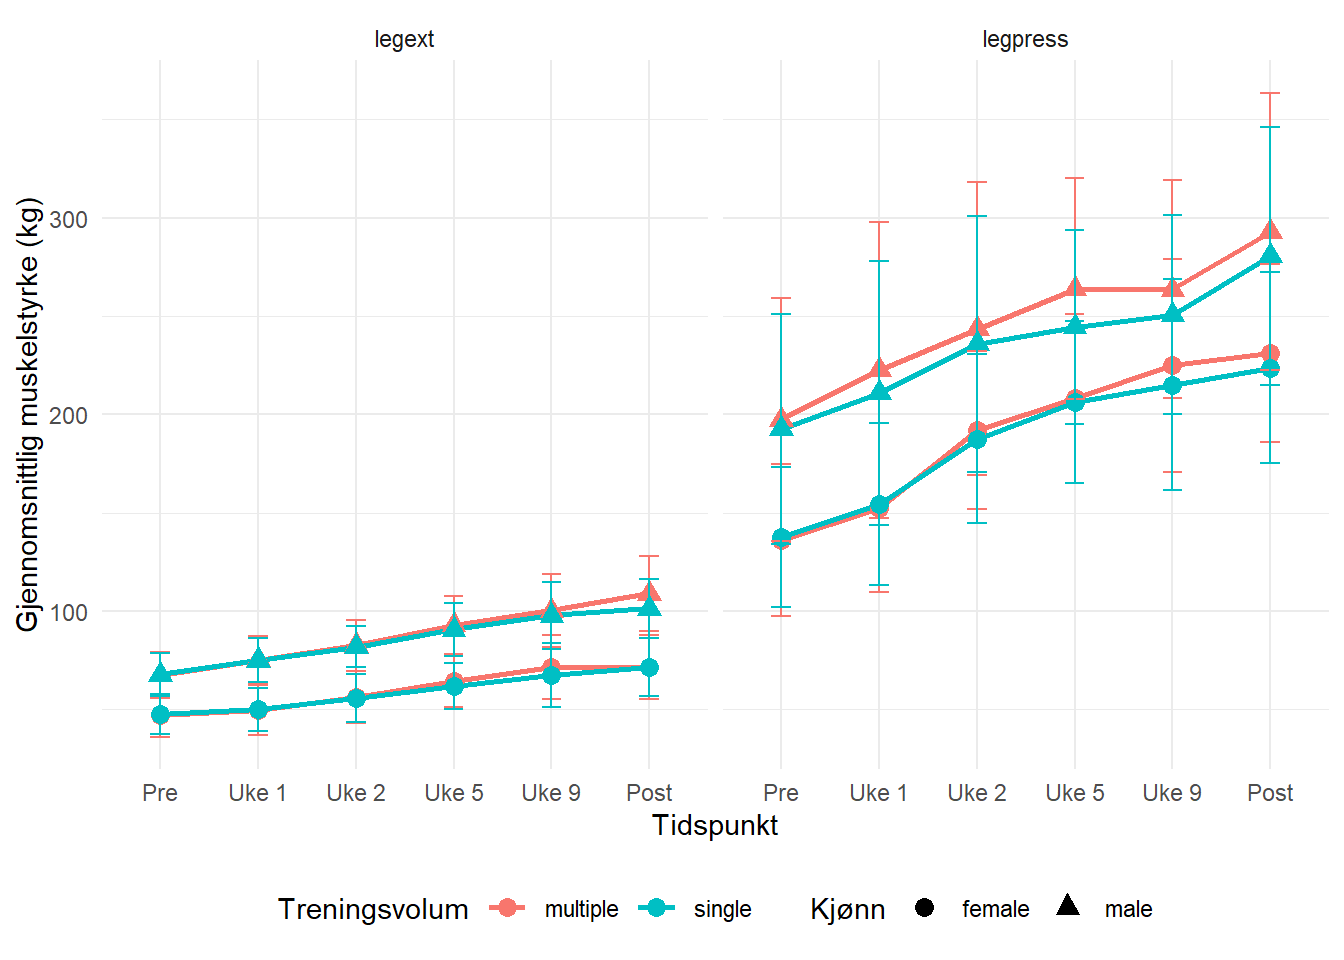
\includegraphics[keepaspectratio]{05-repeated-measurements_files/figure-pdf/fig-styrke-1.pdf}}

}

\caption{\label{fig-styrke}Utvikling i muskelstyrke for leg press og leg
extension.}

\end{figure}%

\section{Endring i muskeltverssnitt}\label{endring-i-muskeltverssnitt}

Resultatene viste en signifikant økning i muskelens tverrsnittsareal
etter treningsperioden (Table~\ref{tbl-muskeltverr}). Den estimerte
koeffisienten for post-testen var 289.88 g (SE = 55.05), med et 95 \%
konfidensintervall fra 181.99 til 397.76. Dette indikerer at deltakerne
i gjennomsnitt økte muskelens tverrsnittsareal med 289,88 gram etter
intervensjonen.

Analysen av effekten av treningsvolum på muskelens tverrsnittsareal
viste at interaksjonen mellom tid og antall sett ikke var signifikant
(estimat = -118.17, SE = 77.37, 95~\% KI {[}-269.82, 33.48{]}, p =
0,13). Dette indikerer at det ikke var en statistisk signifikant
forskjell (p \textgreater{} 0,05) i økningen av muskelens
tverrsnittsareal mellom deltakerne som utførte ett sett og de som
utførte tre sett. Selv om estimatet var negativt, tyder det på at økt
treningsvolum ikke nødvendigvis førte til en større økning i muskelens
tverrsnittsareal i denne studien.

\begin{longtable}[]{@{}
  >{\raggedright\arraybackslash}p{(\linewidth - 6\tabcolsep) * \real{0.1250}}
  >{\raggedright\arraybackslash}p{(\linewidth - 6\tabcolsep) * \real{0.1750}}
  >{\raggedleft\arraybackslash}p{(\linewidth - 6\tabcolsep) * \real{0.4625}}
  >{\raggedleft\arraybackslash}p{(\linewidth - 6\tabcolsep) * \real{0.2375}}@{}}

\caption{\label{tbl-muskeltverr}Oppsummering av muskeltverrsnitt før og
etter intervensjon (kombinert for kjønn, kun pre og post)}

\tabularnewline

\toprule\noalign{}
\begin{minipage}[b]{\linewidth}\raggedright
Tidspunkt
\end{minipage} & \begin{minipage}[b]{\linewidth}\raggedright
Treningsvolum
\end{minipage} & \begin{minipage}[b]{\linewidth}\raggedleft
Gjennomsnittlig muskeltverrsnitt (g)
\end{minipage} & \begin{minipage}[b]{\linewidth}\raggedleft
Standardavvik (SD)
\end{minipage} \\
\midrule\noalign{}
\endhead
\bottomrule\noalign{}
\endlastfoot
post & multiple & 9093.368 & 1297.290 \\
post & single & 8983.975 & 1219.944 \\
pre & multiple & 8835.974 & 1189.980 \\
pre & single & 8845.317 & 1175.207 \\

\end{longtable}

\bookmarksetup{startatroot}

\chapter{Diskusjon}\label{diskusjon-3}

Denne studien undersøkte effekten av to ulike treningsvolum, ett sett
versus tre sett, på muskelstyrke og muskeltverrsnittsareal. Resultatene
viste en signifikant økning i både muskelstyrke og
muskeltverrsnittsareal etter treningsperioden for begge gruppene.
Imidlertid var det ingen statistisk signifikante forskjeller mellom
gruppene som utførte ett sett og de som utførte tre sett, verken for
muskelstyrke eller muskelhypertrofi. De diagnostiske analysene bekreftet
at modellforutsetningene var rimelig oppfylt, noe som gir tillit til
validiteten av funnene våre. Ingen betydelige avvik ble observert i
residualene, og modellene ble derfor ansett som passende for dataene.

Disse funnene utfordrer den etablerte oppfatningen om at et høyere
treningsvolum alltid fører til større muskeltilpasninger. Tidligere
forskning har ofte indikert et dose-respons-forhold mellom treningsvolum
og muskelvekst, hvor økt volum er assosiert med større hypertrofi og
styrkeøkninger ((\textbf{schoenfeld2016?}); (\textbf{currier2023?})).
For eksempel fant Schoenfeld et al.~(2016) at flere sett per øvelse var
mer effektive for muskelhypertrofi enn ett sett. På den annen side har
noen studier ikke funnet signifikante forskjeller mellom ulike
treningsvolum, spesielt når treningsintensiteten er kontrollert
((\textbf{ralston2017?})).

En mulig forklaring på våre funn er at begge treningsvolumene var
tilstrekkelige for å fremkalle maksimale adaptasjoner innenfor den gitte
treningsperioden. Det kan være en terskelverdi for hvor mye volum som er
nødvendig for å stimulere muskelvekst og styrke, og at denne terskelen
ble nådd med ett sett i vår studie. Dette er også sett i forskning som
antyder at selv lave til moderate treningsvolumer kan være effektive for
muskelhypertrofi hos utrente individer ((\textbf{Krieger2010?});
(\textbf{Schoenfeld2019?})).

Når det gjelder muskelstyrke, viste begge gruppene betydelige
forbedringer uten signifikante forskjeller mellom volumene. Dette kan
skyldes at styrkeøkninger i stor grad påvirkes av nevromuskulære
tilpasninger, spesielt i de tidlige stadiene av treningsintervensjoner
((\textbf{Folland2007?})). Det er mulig at den relativt korte
treningsperioden i vår studie ikke var tilstrekkelig for å avdekke
forskjeller i styrkeøkninger basert på treningsvolum.

\section{Begrensninger}\label{begrensninger}

Flere begrensninger bør tas i betraktning. For det første var
utvalgsstørrelsen begrenset, noe som kan ha redusert studiens
statistiske styrke til å oppdage mindre forskjeller mellom gruppene.
Selv om forhåndsberegningen av utvalgsstørrelse indikerte tilstrekkelig
kraft, kan individuelle variasjoner ha påvirket resultatene. For det
andre var treningsperioden relativt kort, og lengre intervensjoner kan
være nødvendig for å observere de fulle effektene av ulikt treningsvolum
på muskelhypertrofi og styrke. I tillegg ble ikke faktorer som kosthold,
søvn og daglige aktiviteter kontrollert, noe som kan ha påvirket
muskeltilpasningene.

\section{Implikasjoner for fremtidig
forskning}\label{implikasjoner-for-fremtidig-forskning}

Fremtidige studier bør vurdere å inkludere større og mer varierte
utvalg, samt lengre treningsperioder, for å bedre forstå effekten av
treningsvolum på muskeltilpasninger. Det kan også være verdifullt å
undersøke hvordan ulike populasjoner, som erfarne idrettsutøvere versus
nybegynnere, responderer på forskjellige treningsvolum. Videre bør
fremtidig forskning ta hensyn til andre treningsvariabler som
intensitet, frekvens og type øvelser for å gi en mer helhetlig
forståelse av optimal treningsdesign.

\section{Konklusjon}\label{konklusjon-1}

Resultatene fra denne studien indikerer at både ett sett og tre sett med
styrketrening fører til signifikante økninger i muskelstyrke og
muskeltverrsnittsareal hos voksne individer. Mangelen på signifikante
forskjeller mellom de to treningsvolumene antyder at et lavere volum kan
være like effektivt som et høyere volum for å fremme muskelstyrke og
hypertrofi i en kortere treningsperiode. Disse funnene har praktiske
implikasjoner for treningsprogrammering, spesielt for individer med
begrenset tid til trening. Likevel er det behov for ytterligere
forskning for å bekrefte disse resultatene og for å utforske de
langsiktige effektene av treningsvolum på muskeltilpasninger.

\bookmarksetup{startatroot}

\chapter{Vitenskapsteori}\label{vitenskapsteori}

\bookmarksetup{startatroot}

\chapter{Arbeidskrav i
filosofihistorie}\label{arbeidskrav-i-filosofihistorie}

\section{Spørsmål 1}\label{spuxf8rsmuxe5l-1}

\emph{``Ifølge Hume er det umulig å rasjonelt begrunne bruken av
induksjon. Hva er argumentet for denne konklusjonen? Gi en innvending
mot ett av premissene i Humes argument og prøv å svare på denne
innvendingen på Humes vegne.''}

\subsection{Innledning}\label{innledning-1}

David Hume var ein skotsk empirist, som gjennom sitt syn og tankar har
hatt stor innflytelse på moderne vitskapsfilosofi (Norton, D. F., \&
Taylor, J. (2008), kap 1). Sjølv om Hume sine meningar og tankar har
vekket ein rekkje spørsmål og debatter frå hans levetid til nå, er det
nok hans skepsis og analyse av årsak og induksjon som har fått mest
merksemd (Norton, D. F., \& Taylor, J., s.214-221).

\subsection{Humes argument mot
induksjon}\label{humes-argument-mot-induksjon}

Induksjon er ein vitskapleg metode som forsøker å trekke generelle lovar
eller prinsipp basert på enkelte observasjonar (Tranøy, 2021), for
eksempel: ``Eg brand meg når eg tok på flammene, derfor er flammer
varme.''. Hume mente at det ikkje er mogleg å fastslå årsaksforholdet
som vi erfarer gjennom sansane våre, som eksempelet med flammene over,
men på grunn av vår gjentatte erfaring med at det er ein konstant
samanheng mellom to typar hendingar, så antar vi at det eine er årsaka
til den andre (Hume, 2019, s.27-28).

Ein forutsetning for at konklusjonen i mitt induktive argument over skal
holde, er at det ikkje skjer ein endring i naturens gang. Denne
førestillinga om likskap mellom observerte (fortida) og uobserverte
mønster (framtida), er kjent som uniformitetsprinsippet. Men, korleis
kan mine tidlegare erfaringar med å brenne meg ved berøring av flammer
legitimere ein slutning om at dette også vil inntreffe i framtida? Hume
hevda at førestillinga om at framtida vil vere lik fortida ikkje kan
bevisast utan å ende i ein sirkulær argumentasjon (Norton, D. F., \&
Taylor, J., s.215). Dette skyldast at for å rettferdiggjere induksjon må
man allereie forutsette det prinsippet man prøver å bevise, at framtida
vil følgje same mønster som fortida.

Hume hevdet at alle induktive argumenter bygger på førestillinga at
framtidige hendingar vil følgje same mønster som tidlegare hendingar, og
at denne førestillinga er ein forutsetning for å trekke induktive
slutningar (Norton \& Taylor, 2008, s.215; Hume, 2019, s.38-39). Når eg
konkluderer med at eg vil brenne meg når eg tar på flammer, baserer eg
denne slutninga på førestillinga om at framtida vil likne på fortida.
Hume påpekte at dette fører til ein sirkulær argumentasjon, sidan eg
ikkje kan bevise min førestilling utan å allereie forutsette same
mønsteret. Dette utgjer sjølve kjernen i Humes kritikk av induksjon, med
at man kan ikkje rasjonelt grunngi bruken av induksjon utan å byggje på
den same førestillinga vi forsøker å bevise.

\subsection{Innvending mot Hume sitt
argument}\label{innvending-mot-hume-sitt-argument}

Selv om Hume påpeikte at vi ikkje kan observere eit nødvendige
årsaksforhold mellom to hendingar, berre at ein hending følgjer ein
anna, kan det innvendast mot dette premisset at naturvitskapen har vist
at induktive slutningar fungerer påliteleg i praksis. For eksempel kan
Newtons gravitasjonslov brukast til å forutsi at ein gjenstand vil falle
mot jorda når den den har blitt sleppt. Sjølv om det kan vere vanskeleg
å bevise nødvendige årsaksforhold direkte, kan ein hevde at den
praktiske suksessen til naturvitskaplege lover, som Newtons
gravitasjonslov, rettferdiggjer bruken av induksjon. Dette kjem tydeleg
til uttrykk i vår evne til nøyaktig å forutsi framtidige hendingar, som
planetbanar eller gjenstandar sin bevegelse på jorda, basert på
tidlegare erfaringar.

\subsection{Humes respons på
innvendinga}\label{humes-respons-puxe5-innvendinga}

Hume ville sannsynlegvis ha svart på innvendinga ved å fasthalde sin
skepsis til at induksjon er basert på rasjonell fornuft. I staden ville
han ha påpeikt at våre induktive slutningar kjem frå ein naturlig
tilbøyelegheit til å forvente at framtida vil likne fortida, basert på
vaner og førestellingsevne (Hume, 2019, s.48-49). Denne tilbøyelegheita
til å trekke slutningar om framtida er det Hume kalte for customs, altså
vaner (Hume, 2019, s.44). Sjølv om Hume ville ha oppretthaldt sin
påstand om at induksjon ikkje er rasjonelt grunngitt, ville han også ha
erkjent, i likskap med min innvending, at induksjon er avgjerande for
vår praktiske suksess. Hume meinte at desse induktive slutningane, som
bygger på vaner og erfaringar, er meir effektive for vår overleving og
praktiske handlingar enn om vi skulle ha basert alle slutningar på rein
rasjonalitet (David, H., 2019, s.57-58).

\section{Spørsmålet 2}\label{spuxf8rsmuxe5let-2}

\emph{Gi en kort beskrivelse av falsifikasjonisme og si litt om hvorfor
Popper var motivert til å utvikle denne teorien. Presenter så ett
problem med teorien og vurder hvorvidt problemet kan løses.}

\subsection{Innledning}\label{innledning-2}

Demarksjonsproblemet er eit grunnleggande tema innan vitskapsfilosofien,
og det handlar om korleis vi kan skilje mellom vitskap og ikkje-vitskap.
Dette skiljet er avgjerande for vår forståing av kva som reiknast som
gyldig kunnskap, og har implikasjonar for områder som metafysikk og
religion (Popper, K. R., 1959, s.34-39). Mange filosofer har forsøkt å
definere klare kriterier for denne avgrensinga, og ein dei mest sentrale
i denne debatten er Karl Popper.

\subsection{Beskrivelse av falsifikasjonisme og Poppers
motivasjon}\label{beskrivelse-av-falsifikasjonisme-og-poppers-motivasjon}

Popper var ein markant kritikar av induksjon. Gjennom sin avvising av
induksjonsprinsippet utfordra han ikkje berre empirisk vitskap sin
grunnleggande metode, men også det tradisjonelle skiljet mellom vitskap
og metafysisk spekulasjon (Popper, K. R., 1959, s.34). For Popper var
ein vitskapeleg teori ikkje gyldig fordi den kunne verifiserast gjennom
observasjonar, men fordi den kunne falsifiseres gjennom testing (Popper,
K. R., 1959, s.40). Han hevdet at vitskapens rolle er ikkje å verifisere
ein teori basert på enkeltobservasjonar eller erfaring, men å utvikle
teoriar som kunne falsifiseres gjennom observasjonar eller eksperimenter
(Popper, K. R., 1959, s.41-42, 47-48).

Eit eksempel på ein vitskapelig teori er påstanden: ``Newton sin lov om
gravitasjon seie at steinen eg slipp vil falle mot bakken på grunn av
tiltrekkinga mellom to masser.''. Denne påstanden er vitskapeleg fordi
den kan testast og potensielt falsifiseres. Derimot vil påstanden
``Steinen faller fordi universet bestemmer det.'', ikkje kunne
falsifiseres og er dermed ikkje vitskapeleg.

Popper var motivert til å utvikle falsifikasjonismen på grunn av dei
svakheitene han såg i induktiv logikk. Han meinte at ideen om at
generaliseringar basert på observasjonar kunne gi sikker kunnskap, var
logisk problematisk. Som eit svar på dette utvikla han
falsifikasjonsprinsippet, som metode for å sikre at teoriar kunne
utfordrast og testast på ein måte som kunne avsløre deires potensielle
moglegheiter for feil.

\subsection{Utfordring med
falsifikasjonisme}\label{utfordring-med-falsifikasjonisme}

Sjølv om Popper sin falsifikasjonisme gir ein streng vitskapleg metode,
gjenspeglar den ikkje alltid korleis vitskap faktisk utviklar seg.
Ifølge Popper bør ein teori forkastast når den møter motstridne data,
ettersom den då er falsifisert og dermed ``bevist'' å gjere feil. Popper
var kritisk til bruken av tilpassingar og hjelpehypotesar som berre ble
introdusert for å redde teoriar frå falsifikasjon, fordi dette kunne
redusere falsifiserbarheita til teorien og dermed gjere den uvitskapleg
(Popper, K. R., 1959, s.145).

I praksis er det sjeldan forskarar forkastar ein teori ved første teikn
til motstridene data. Ofte vel dei å gjere tilpassingar eller forbetrar
teoriane med hjelp av hjelpehypotesar. Dette skaper derfor eit
misforhold mellom Popper sitt ideal om falsifikasjon og vitskapleg
praksis, der teoriar ofte justerast i staden for å bli forkasta
umiddelbart. Eit eksempel på dette er Newton sine lover om bevegelse,
som ble revidert fleire gangar gjennom historia. Sjølv om Newtons lover
forklarte bevegelse i dei fleste praktiske situasjonar med høy
presisjon, viste dei seg utilstrekkelege for å beskrive bevegelse i
ekstreme forhold som ved svært høge hastigheiter. I staden for å
forkaste lovene, ble dei utvida og korrigert av Albert Einstein for å
forklare avvika. Dette er eit eksempel på korleis vitskapen i praksis
ofte justerer teoriar framfor å forkaste dei umiddelbart.

\subsection{Poppers løsning}\label{poppers-luxf8sning}

Popper erkjenner denne utfordringa, men hevder at ho kan løysast ved å
følgje strenge metodologiske regler (Popper, 1959, s.81-84, 145). Han
argumenterer for at tilpassingar som berre løyser eit enkelt problem i
ein teori, såkalla ad hoc-hypotesar, bør unngåast, da dei svekkjer
teoriens vitskaplege verdi. Modifikasjonar som fører til nye, testbare
predikasjonar er derimot akseptable, ettersom dei styrkjer teorien ved å
gjere den meir falsifiserbar (Popper, 1959, s.83). Vidare framhevar
Popper prinsippet om sparsommeligheit, kjent som Ockhams barberkniv, som
tilseier at man bør unngå unødvendig antakingar for å forhindre at
teoriar blir unødig komplekse (Store norske leksikon, 2005-2007).

Sjølv om disse reglene gir ein metodologiske løysning på problemet, kan
dei vere betre eigna som ideal enn som praktiske verktøy i vitskapeleg
praksis. Vitskapen i praksis er meir fleksibel og kompleks enn det
Popper førestilte seg, og det er ikkje like enkelt å vite når man bør
forkaste ein teori og når man burde revidere den.

\subsection{Konklusjon}\label{konklusjon-2}

Sjølv om falsifikasjonisme i teorien seie at ein teori skal forkastast
ved motstridande data, viser vitskapleg praksis at teoriar ofte
modifiserast og tilpassast i staden. Dette reflekterer vitskapens natur
som ein kontinuerleg prosess med prøving, feil, og forbetring, og at
falsifikasjon i praksis viser seg å vere ein meir gradvis og fleksibel
prosess enn det Poppers opprinnelege modell antydar.

\bookmarksetup{startatroot}

\chapter{Laboratory Report}\label{laboratory-report}

\section{Introduksjon og bakgrunn}\label{introduksjon-og-bakgrunn}

I jakten på å oppnå en dypere forståelse av de molekylære reaksjonene
som regulerer transkripsjon og translasjon med trening, ernæring, sykdom
og aldring, har bruken av Western blot (WB) i treningsfysiologi økt. WB
er en sentral metode for å undersøke regulatoriske molekylære
reaksjoner, blant annet ved å kvantifisere proteinmengder og analysere
protein-protein-interaksjoner. Dette er avgjørende for å kunne
dokumentere fysiologiske adaptasjoner som oppstår som respons til
trening (Bass et al. 2017).

Western blot har tradisjonelt vært assosiert med overføring av proteiner
fra en gel til en stabil membran, men idag referer metoden til hele
prosessen, fra proteinekstraksjon til kvantitativ analyse (Bass et al.
2017, s.2). Prosessen inkluderer ekstraksjon av proteiner, seperasjon
ved elektroforese, overføring til en membran, blokking for å hindre
uspesifikke bindinger, og påføring av antistoffer for å identifisere
proteiner. Til slutt kvantifiseres proteinmengdene ved hjelp av
densiometrisk programvare (Bass et al. 2017).

p70S6K er en nøkkelkomponent i mTORC1-signalveien, som spiller en
sentral rolle i reguleringen av proteinsyntese og muskelvekst (D'Souza
and al. 2014, s.7). Singalveien aktiveres som respons på mekanisk
belastning, og er avgjørende for muskulære tilpasninger til trening
(Atherton and Smith 2012). Fosforlyering av p70S6K er en indikator på
aktivering av mTORC1, som igjen reflekterer cellulære prosesser som
fremmer anabole responser i muskulaturen (D'Souza and al. 2014; Holz and
al. 2005, s.577--579). Ved å måle både totalmengden av p70S6K og den
fosforylerte formen kan man få innsikt i balansen mellom inaktive og
aktive proteiner, noe som gir et mer helhetlig bilde av signalveiens
funksjon (Bass et al. 2017). Derfor er p70S6K et ideelt mål for å
studere molekylære tilpasninger til trening.

Formålet med dette eksperimentet er å bruke og demonstrere Western Blot
som en metode for å analysere proteinuttrykk. Dette gjøres ved å
sammenligne totalmengden av p70S6K (t-p70) og mengden fosforylert p70S6K
i muskelvev fra et ben som har gjennomført en styrketreningsøkt, med et
ben som ikke har trent, over tid etter treningen. Ved å sammenligne det
trenede og utrenede ønsker man å evaluere hvordan trening påvirker
aktiveringen av mTORC1-signalveien, og samtidig demonstrere hvordan WB
kan brukes til å undersøke slike molekylær mekanismer.

\section{Metode}\label{metode-6}

Muskelprøvene som ble brukt i dette eksperimentet, ble hentet fra m.
vastus lateralis på høyre og venstre lår hos testpersoner. Høyre ben
gjennomførte styrketrening, mens venstre ben fungerte som kontroll.
Prøvene ble samlet inn på ulike tidspunkter etter trening for å vurdere
tidsavhengige endringer: én prøve ble tatt 10 minutter etter trening
(HE), en annen 30 minutter etter (LØ), og den siste 60 minutter etter
(T). Før Western blot (WB)-analysen ble muskelprøvene homogenisert for å
frigjøre proteiner. Fremgangsmåten for homogenisering og WB er detaljert
beskrevet i den følgende delen. Kodene som er blitt brukt for å lage
tabeller ligger vedlagt nederst under overskriften ``Koder'', som ligger
etter konklusjonen.

\subsection{Homogenisering av
muskelprøver}\label{homogenisering-av-muskelpruxf8ver}

Prøvene ble veid før homogenisering, og vekten for testperson HE var
henholdsvis 14,0 μg for høyre ben (HE-R) og 14,5 μg for venstre ben
(HE-L). Til homogeniseringen ble 600 μl lysisbuffer tilsatt, sammensatt
av 594 μl T-PER (Thermo Fisher Scientific) og 6 μl Pink Reagent for å
indikere homogeniseringens fullstendighet. En plastpistill ble brukt til
å mekanisk bryte ned vevet til en homogen løsning.

Homogenisering ble utført ved hjelp av en plastpistill for å bryte ned
vevet og frigjøre proteinene. Til dette brukte vi 600 μl lysisbuffer,
bestående av 594 μl T-PER og 6 μl Pink Reagent for å sikre at vevet ble
fullstendig homogenisert. Den homogeniserte prøven ble deretter
behandlet for å måle proteinkonsentrasjonen ved hjelp av Bradford
Assay-metoden.

Prøvene ble holdt på is under behandlingen og rotert i 33 minutter for å
sikre tilstrekkelig homogenisering. Etter homogeniseringen ble prøvene
sentrifugert ved 10 000 g i 10 minutter ved 4 °C for å separere
supernatanten fra pelleten. Supernatanten ble deretter forsiktig
overført til et nytt rør for å unngå forstyrrelse av pelleten. Denne
prosessen gikk uten problemer og med minimal sannsynlighet for
feilkilder.

For å måle proteinkonsentrasjonen ble det utført en fortynning av
prøvene. En fortynning på 1:6 ble brukt for å bringe homogenatet
innenfor standardkurvens område. Dette innebar at 12 μl prøve ble
blandet med 60 μl destillert vann. Pipetteringen ble utført nøye og uten
merkbare feil, selv om mulige feilkilder alltid må vurderes.

Bradford Assay-metoden benytter fargestoffet Coomassie Brilliant Blue
G-250, som binder seg til proteiner og gir en fargeendring som er
proporsjonal med proteinkonsentrasjonen (Noble and Bailey 2008). For å
kvantifisere proteinkonsentrasjonen laget vi en standardkurve basert på
bovint serumalbumin (BSA), som fungerer som en referanse. Absorbansen
til prøvene ble målt ved 595 nm ved hjelp av et spektrofotometer. Dette
gjorde det mulig å fastslå om prøvene inneholdt lave eller høye
konsentrasjoner av proteiner, med grunnlag i sammenligning med
standardkurven (Noble and Bailey 2008, kap 8).

\subsection{Western blot protokoll}\label{western-blot-protokoll}

Selv om gruppen jobbet med en prøve, er WB-analysen blitt gjort på flere
prøver fra 3 ulike testpersoner. For elektroforesen brukte vi Bio-Rad
Criterion og en ferdiglaget gel. Selv om det ikke ble brukt en
kalibreringskurve for å kvantifisere absolutt mengde p70S6K, ble
intensitetsverdiene normalisert mot total proteinmengde og deretter
brukt som en indikator for proteinaktivitet. Fosforyleringsnivået
(p−p70/t−p70p) ble beregnet for å gi et relativt mål på aktivering av
mTORC1-signalveien.

De homogeniserte prøvene ble fortynnet til en endelig konsentrasjon på
1.5-2 μg/μl i Laemmli-bufer (Bio-Rad). Prøvene ble deretter denaturert
ved oppvarming til 95 °C i 5 minutter før de ble avkjølt til
romtemperatur. Proteinstandarder (Precision Plus Protein Dual Color
Standards, fra Bio-Rad) ble brukt for å sikre nøyaktig beregning av
proteinstørrelse. Prøvene ble lastet på en ferdiglaget Bio-Rad
Criterion-gel, og elektroforese ble utført ved konstant spenning (300 V)
i 30 minutter ved 4 °C, med bruk av Bio-Rad Running Buffer.

En potensiell feil ble identifisert under prøvelastingen i brønn 5, hvor
en prøve utilsiktet ble trukket tilbake i pipetten. Selv om alle væske
ble overført til brønnen, kan dette ha resultert i blanding. Oversikt
over de ulike brønnene er vist i Table~\ref{tbl-pipe}, der brønn 2-6 er
p-p70 og brønn 9-13 er t-p70.

\begin{table}

\caption{\label{tbl-pipe}Distribusjon av prøvene.}

\centering{

\caption*{
{\large Western Blot Brønndistribusjon}
} 
\fontsize{12.0pt}{14.4pt}\selectfont
\begin{tabular*}{\linewidth}{@{\extracolsep{\fill}}cc}
\toprule
Brønn & Innhold \\ 
\midrule\addlinespace[2.5pt]
1 & M \\ 
2 & HE-L \\ 
3 & HE-R \\ 
4 & T-L \\ 
5 & T-R \\ 
6 & LØ-R \\ 
7 & M \\ 
8 & M \\ 
9 & HE-L \\ 
10 & HE-R \\ 
11 & T-L \\ 
12 & T-R \\ 
13 & LØ-R \\ 
14 & M \\ 
\bottomrule
\end{tabular*}
\begin{minipage}{\linewidth}
Forklaringer: M = Markør, HE-L = Venstre ben (10 min), HE-R = Høyre ben (10 min), T-L = Venstre ben (60 min), T-R = Høyre ben (60 min), LØ-R = Høyre ben (30 min)\\
\end{minipage}

}

\end{table}%

Etter elektroforese ble prøvene først lagt i metanol i 2-10 minutter,
for å gjøre det mulig for proteinene å binde seg mer effektivt. Deretter
ble de overført til en PVDF-membran ved hjelp av en ``wet
blotting''-metode, hvor proteine ble drevet ut av gelen og overført til
membranen under påvirkning av en elektrisk strøm i en bufferløsning
(Bass et al. 2017, s.10--12).Selve overføringen skulle etter protokollen
bli utført ved konstant strøm (300 mA) i 3 timer ved romtemperatur, med
en buffer bestående av 25 mM Tris, 192 mM glycin og 20\% metanol, hvor
metanol hjalp til med å stabilisere proteinene. Grunnet mangelende tid,
ble det heller kjørt et hurtigprogram (100 V i 30 minutter). Dette kan
ha redusert effektiviteten for større proteiner. Membranet ble deretter
farget med MemCode Reversible Protein Stain for å visualisere om
proteinene var blitt overført og jevnt fordelt. Fargingen ga også
mulighet til å visualisere total proteinmengde og justere for
variasjoner mellom prøvene i den neste analysen.

Membranen ble blokkert i en 5 \% melkebuffer (TBS-T) i 1 time ved
romtemperatur for å redusere ikke-spesifikk binding. Primærantistoffet
mot fosforylert p70S6K (p-p70S6K) ble inkubert over natten ved 4 °C, og
deretter vasket grundig med TBS-T for å fjerne overskuddsantistoff.
Sekundærantistoffet ble tilsatt i 2.5 \% melkebuffer og inkubert i 1
time ved romtemperatur. Ufullstendig vask under dette trinnet kan ha
ført til bakgrunnsstøy, da vaskingen ble utført av en annen person.

For å få frem signalene ble det benyttet ECL (Enhanced
Chemiluminesscence) og bildeopptak på en Gel Doc-enhet (Bass et al.
2017, s.18--19). Kvantifisering av Western blot-resulatetene ble utført
ved hjelp av densiometrisk analyse i programmet ImageJ. Den høyeste
intensiteten av proteinbåndene for p-p70S6K og t-p70S6K ble målt og
normalisert mot total proteinmengde for å korrigere for variasjoner i
prøvene (Bass et al. 2017, s.20--24). Forholdet mellom p-p70S6K og
t-p70S6K ble beregnet som en indikator på aktiveringen av
mTORC1-signalveien.

De ulike løsningene som er blitt brukt, er listet opp nederst i oppgåven
etter konklusjon.

\section{Resultater}\label{resultater-2}

Vi benyttet oss av WB-analyse for å kvantifisere total p70S6K og
fosforlyert p70S6K, slik at vi kunne undersøke fosforyleringsnivået til
proteinet i vastus lateralis til de ulike testpersonene. Intensiteten
til fosforylert p70S6K (p-p70) og total p70S6K (t-p70) ble normalisert
mot totalprotein fra membran blottet. Fosforyleringsnivået ble beregnet
som forholdet mellom p-p70 og t-70 (p-p70 / t-p70). Intensitetsverdiene
som presenteres i tabellene er basert på optisk tetthet fra Western
blot-bildene. Verdiene representerer relative signalstyrker og har ingen
absolutt måleenhet, da kalibreringskurve ikke ble benyttet. For å
korrigere for variasjoner i proteinmengde mellom brønnene, f.eks grunnet
pipeteringsfeil eller feil i total protein-målinger, ble intensitetene
normalisert mot total proteinmengde (membran blot).

I Table~\ref{tbl-WB} vises de normaliserte intensitetsverdiene for
fosforylert (p-p70) og total (t-p70) p70S6K for høyre og venstre bein
hos hver testperson, basert på membran blottet. Fosforyleringsnivået er
beregnet som forholdet mellom normalisert p-p70 og t-p70.
Fosforyleringsnivået (p-p70/t-p70) varierte mellom prøvene, med høyest
nivå i trent bein hos testperson T (1.550) og lavest i utrent bein hos
testperson LØ (0.920).

\begin{table}

\caption{\label{tbl-WB}Intensitetsverdiene for p-p70S6K og t-p70S6K fra
densiometer analysen i ImageJ.}

\centering{

\caption*{
{\large Western Blot analyse av fosforyleringsnivå}
} 
\fontsize{12.0pt}{14.4pt}\selectfont
\begin{tabular*}{\linewidth}{@{\extracolsep{\fill}}ccccccccc}
\toprule
{\cellcolor[HTML]{ADD8E6}{Testperson}} & {\cellcolor[HTML]{ADD8E6}{Bein}} & {\cellcolor[HTML]{ADD8E6}{Membran blot (p-p70)}} & {\cellcolor[HTML]{ADD8E6}{Membran blot (t-p70)}} & {\cellcolor[HTML]{ADD8E6}{p-p70 (raw)}} & {\cellcolor[HTML]{ADD8E6}{t-p70 (raw)}} & {\cellcolor[HTML]{ADD8E6}{p-p70 (norm.)}} & {\cellcolor[HTML]{ADD8E6}{t-p70 (norm.)}} & {\cellcolor[HTML]{ADD8E6}{Fosforyleringsnivå}} \\ 
\midrule\addlinespace[2.5pt]
HE & Venstre & 16 530.47 & 15 516.16 & 4 276.45 & 4 276.45 & 0.26 & 0.28 & 0.94 \\ 
HE & Høgre & 10 135.43 & 13 009.67 & 4 238.28 & 4 238.28 & 0.42 & 0.33 & 1.28 \\ 
T & Venstre & 11 187.97 & 12 917.48 & 4 457.28 & 4 457.28 & 0.40 & 0.34 & 1.16 \\ 
T & Høgre & 7 012.39 & 10 868.74 & 4 148.45 & 4 148.45 & 0.59 & 0.38 & 1.55 \\ 
LØ & Høgre & 14 791.04 & 13 617.43 & 4 249.86 & 4 249.86 & 0.29 & 0.31 & 0.92 \\ 
\bottomrule
\end{tabular*}
\begin{minipage}{\linewidth}
Merk: Tallene er råverdier uten en spesifikk enhet.\\
\end{minipage}

}

\end{table}%

Den gjennomsnittlige aktiviteten til p70S6K i hele gruppen var 1.17 ±
0.25. Det trente beinet hadde et høyere fosforyleringsnivå (1.43 ± 0.15)
enn det utrente beinet (0.99 ± 0.09). Disse funnene indikerer at
mekanisk belastning fra treningen førte til økt aktivering av
mTORC1-signalveien.

Total p70S6K (t-p70) viste en liten forskjell mellom de to gruppene.
Gjennomsnittet for hele gruppen var 0.33 ± 0.04, mens det trente beinet
hadde et noe høyere nivå (0.35 ± 0.04) enn det utrente beinet (0.31 ±
0.03).

For fosforylert p70S6K (p-p70) var forskjellene mer markante.
Gjennomsnittet for hele gruppen var 0.39 ± 0.12, mens nivået i det
trente beinet (0.50 ± 0.12) var betydelig høyere enn i det utrente
beinet (0.31 ± 0.07). Disse resultatene understøtter observasjonen om at
trening spesifikt øker fosforyleringen av p70S6K og aktiverer
mTORC1-signalveien.

\begin{table}

\caption{\label{tbl-resultater}Deskriptiv data fra densiometri
analysen.}

\centering{

\caption*{
{\large Tabell 2: Gjennomsnittlige nivåer av total og fosforylert p70S6K} \\ 
{\small Nivåene er presentert som gjennomsnitt ± standardavvik (SD)}
} 
\fontsize{12.0pt}{14.4pt}\selectfont
\begin{tabular*}{\linewidth}{@{\extracolsep{\fill}}cccc}
\toprule
{\bfseries Parameter} & Hele gruppen
(n = 20) & Høyre bein
(n = 10) & Venstre bein
(n = 10) \\ 
\midrule\addlinespace[2.5pt]
t-p70 (norm.) & 0.33 ± 0.04 & 0.35 ± 0.04 & 0.31 ± 0.03 \\ 
p-p70 (norm.) & 0.39 ± 0.12 & 0.50 ± 0.12 & 0.31 ± 0.07 \\ 
Fosforyleringsnivå & 1.17 ± 0.25 & 1.43 ± 0.15 & 0.99 ± 0.09 \\ 
\bottomrule
\end{tabular*}

}

\end{table}%

\section{Diskusjon}\label{diskusjon-4}

Intensitetsverdiene gir oss et bilde av p70S6K-aktiviteten i prøvene.
Selv om absolutt kvantifisering ikke ble utført, indikerer et høyere
fosforyleringsnivå en økt aktivitet av mTORC1-signalveien, som spiller
en sentral rolle for proteinsyntese (Atherton and Smith 2012).
Resultatene viser et høyere fosforyleringsnivå av p70S6K i det trente
beinet sammenlignet med det utrente, noe som understreker treningens
evne til å stimulere molekylære mekanismer som fremmer muskulær
tilpasning. Aktiveringen ser ut til å være tidsavhengig, med høyest nivå
kort tid etter trening og en gradvis reduksjon over tid, i tråd med
tidligere forskning (Atherton and Smith 2012; D'Souza and al. 2014).

Variasjonen i fosforyleringsnivåene kan tilskrives både biologiske og
tekniske faktorer. Forskjellene mellom høyre og venstre bein var mer
konsistente enn variasjonen på gruppenivå, noe som tyder på en spesifikk
effekt av trening. En viktig begrensning er mangelen på en
kalibreringskurve, som gjør det vanskelig å kvantifisere proteinmengden
absolutt. Dette begrenser muligheten til å sammenligne resultatene
direkte med tidligere studier, men demonstrerer samtidig hvordan Western
blot kan brukes for å undersøke slike mekanismer.

Ved å belyse aktiveringen av mTORC1-signalveien, kan man få en dypere
forståelse av molekylære tilpasninger til trening.

\section{Konklusjon}\label{konklusjon-3}

Resultatene indikerer en asymmetrisk aktivering av mTORC1-signalveien
mellom høyre og venstre bein, noe som kan forklares ved at kun det ene
beinet ble trent før biopsien. Styrketrening førte til en akutt økning i
fosforyleringsnivået av p70S6K, med størst aktivering observert kort tid
etter trening. Dette understreker treningens evne til å stimulere
molekylære mekanismer som fremmer proteinsyntese og muskulær tilpasning.

Selv om resultatene gir innsikt i p70S6K-aktiveringen etter trening, må
de tolkes med forsiktighet på grunn av metodiske begrensninger som
bakgrunnsstøy på blottet, pipetteringsfeil, ujevn proteinoverføring og
mangelen på en kalibreringskurve.

\section{Oppløsninger}\label{oppluxf8sninger}

\begin{table}

\caption{\label{tbl-buffer}Bufferoppløsninger}

\centering{

\caption*{
{\large Oversikt over oppløsninger} \\ 
{\small Tabellen viser bufferløsninger med komponenter, konsentrasjoner og masser.}
} 
\fontsize{12.0pt}{14.4pt}\selectfont
\begin{tabular*}{\linewidth}{@{\extracolsep{\fill}}cccc}
\toprule
Bufferoppløsning & {\bfseries Komponent} & {\bfseries Konsentrasjon (mM)} & {\bfseries Masse (g)} \\ 
\midrule\addlinespace[2.5pt]
TBS 1L 10x, pH 7.6 (HCI adjust) & Tris Base
NaCI & 200 mM
1.37 M & 24.22 g
80.06 g \\ 
Running buffer 1L 10x, pH 8.3 & Tris Base
Glycin
SDS & 250 mM
1.92 M
35 mM & 30.28 g
144.1 g
10.09 g \\ 
Transfer buffer 1L 10x & Tris Base
Glycin & 250 mM
1.92 M & 30.28 g
144.1 g \\ 
\bottomrule
\end{tabular*}
\begin{minipage}{\linewidth}
1 x Transfer buffer = 100 ml TB stock x 10 + 100 ml methanol + 800 ml dH2O\\
\end{minipage}

}

\end{table}%

\section{Koder brukt}\label{koder-brukt}

\begin{table}

\caption{\label{tbl-buffer-vedlegg}}

\centering{

\begin{Shaded}
\begin{Highlighting}[]
\FunctionTok{library}\NormalTok{(gt)}

\CommentTok{\# Opprett datasettet}
\NormalTok{buffer\_data }\OtherTok{\textless{}{-}} \FunctionTok{data.frame}\NormalTok{(}
  \StringTok{\textasciigrave{}}\AttributeTok{Buffer Solution}\StringTok{\textasciigrave{}} \OtherTok{=} \FunctionTok{c}\NormalTok{(}\StringTok{"TBS 1L 10x, pH 7.6 (HCI adjust)"}\NormalTok{, }
                        \StringTok{"Running buffer 1L 10x, pH 8.3"}\NormalTok{, }
                        \StringTok{"Transfer buffer 1L 10x"}\NormalTok{),}
  \StringTok{\textasciigrave{}}\AttributeTok{Komponent}\StringTok{\textasciigrave{}} \OtherTok{=} \FunctionTok{c}\NormalTok{(}
    \StringTok{"Tris Base}\SpecialCharTok{\textbackslash{}n}\StringTok{NaCI"}\NormalTok{,}
    \StringTok{"Tris Base}\SpecialCharTok{\textbackslash{}n}\StringTok{Glycin}\SpecialCharTok{\textbackslash{}n}\StringTok{SDS"}\NormalTok{,}
    \StringTok{"Tris Base}\SpecialCharTok{\textbackslash{}n}\StringTok{Glycin"}
\NormalTok{  ),}
  \StringTok{\textasciigrave{}}\AttributeTok{Konsentrasjon (mM)}\StringTok{\textasciigrave{}} \OtherTok{=} \FunctionTok{c}\NormalTok{(}
    \StringTok{"200 mM}\SpecialCharTok{\textbackslash{}n}\StringTok{1.37 M"}\NormalTok{,}
    \StringTok{"250 mM}\SpecialCharTok{\textbackslash{}n}\StringTok{1.92 M}\SpecialCharTok{\textbackslash{}n}\StringTok{35 mM"}\NormalTok{,}
    \StringTok{"250 mM}\SpecialCharTok{\textbackslash{}n}\StringTok{1.92 M"}
\NormalTok{  ),}
  \StringTok{\textasciigrave{}}\AttributeTok{Masse (g)}\StringTok{\textasciigrave{}} \OtherTok{=} \FunctionTok{c}\NormalTok{(}
    \StringTok{"24.22 g}\SpecialCharTok{\textbackslash{}n}\StringTok{80.06 g"}\NormalTok{,}
    \StringTok{"30.28 g}\SpecialCharTok{\textbackslash{}n}\StringTok{144.1 g}\SpecialCharTok{\textbackslash{}n}\StringTok{10.09 g"}\NormalTok{,}
    \StringTok{"30.28 g}\SpecialCharTok{\textbackslash{}n}\StringTok{144.1 g"}
\NormalTok{  ),}
  \AttributeTok{check.names =} \ConstantTok{FALSE}
\NormalTok{)}

\CommentTok{\# Lag tabellen med \textasciigrave{}gt\textasciigrave{}}
\NormalTok{buffer\_table }\OtherTok{\textless{}{-}}\NormalTok{ buffer\_data }\SpecialCharTok{\%\textgreater{}\%}
  \FunctionTok{gt}\NormalTok{() }\SpecialCharTok{\%\textgreater{}\%}
  \FunctionTok{tab\_header}\NormalTok{(}
    \AttributeTok{title =} \StringTok{"Oversikt over oppløsninger"}\NormalTok{,}
    \AttributeTok{subtitle =} \StringTok{"Tabellen viser bufferløsninger med komponenter, konsentrasjoner og masser."}
\NormalTok{  )}
\end{Highlighting}
\end{Shaded}

}

\end{table}%

\bookmarksetup{startatroot}

\chapter*{Referanser}\label{referanser}
\addcontentsline{toc}{chapter}{Referanser}

\phantomsection\label{refs}
\begin{CSLReferences}{1}{0}
\bibitem[\citeproctext]{ref-Atherton2012}
Atherton, P. J., and K. Smith. 2012. {``Muscle Protein Synthesis in
Response to Nutrition and Exercise.''} \emph{The Journal of Physiology}
590 (5): 1049--57. \url{https://doi.org/10.1113/jphysiol.2011.225003}.

\bibitem[\citeproctext]{ref-bartlett2003}
Bartlett, John MS, and David Stirling. 2003. \emph{PCR Protocols:
Methods in Molecular Biology}. Vol. 226. Humana Press.

\bibitem[\citeproctext]{ref-Bass2017}
Bass, John J., Daniel J. Wilkinson, Daniel Rankin, Bethan E. Phillips,
Nathan J. Szewczyk, Kenneth Smith, and Philip J. Atherton. 2017. {``An
Overview of Technical Considerations for Western Blotting Applications
to Physiological Research.''} \emph{Scandinavian Journal of Medicine \&
Science in Sports} 27 (1): 4--25.
\url{https://doi.org/10.1111/sms.12702}.

\bibitem[\citeproctext]{ref-DSouza2014}
D'Souza, R. F., and et al. 2014. {``Dose-Dependent Increases in p70S6K
Phosphorylation and Intramuscular Branched-Chain Amino Acids in Older
Men Following Resistance Exercise and Protein Intake.''}
\emph{Physiological Reports} 2 (8): e12112.
\url{https://doi.org/10.14814/phy2.12112}.

\bibitem[\citeproctext]{ref-RN1739}
Halperin, I., D. B. Pyne, and D. T. Martin. 2015. {``Threats to Internal
Validity in Exercise Science: A Review of Overlooked Confounding
Variables.''} Journal Article. \emph{Int J Sports Physiol Perform} 10
(7): 823--29. \url{https://doi.org/10.1123/ijspp.2014-0566}.

\bibitem[\citeproctext]{ref-Holz2005}
Holz, M. K., and et al. 2005. {``mTOR and S6K1 Mediate Assembly of the
Translation Preinitiation Complex Through Dynamic Protein Interchange
and Ordered Phosphorylation Events.''} \emph{Cell} 123 (4): 569--80.
\url{https://doi.org/10.1016/j.cell.2005.10.024}.

\bibitem[\citeproctext]{ref-RN130}
Hopkins, W. G. 2000. {``Measures of Reliability in Sports Medicine and
Science.''} Journal Article. \emph{Sports Med} 30 (1): 1--15.
\url{http://www.ncbi.nlm.nih.gov/pubmed/10907753}.

\bibitem[\citeproctext]{ref-RN1953}
Ioannidis, John P. A. 2005. {``Why Most Published Research Findings Are
False.''} Journal Article. \emph{PLOS Medicine} 2 (8): e124.
\url{https://doi.org/10.1371/journal.pmed.0020124}.

\bibitem[\citeproctext]{ref-kindermann1979}
Kindermann, W., G. Simon, and J. Keul. 1979. {``The Significance of the
Aerobic-Anaerobic Transition for the Determination of Work Load
Intensities During Endurance Training.''} \emph{European Journal of
Applied Physiology and Occupational Physiology} 42: 25--34.
\url{https://doi.org/10.1007/BF00421101}.

\bibitem[\citeproctext]{ref-machado2012}
Machado, Fabiana Andrade, Fábio Yuzo Nakamura, and Solange Marta Franzói
De Moraes. 2012. {``Influence of Regression Model and Incremental Test
Protocol on the Relationship Between Lactate Threshold Using the
Maximal-Deviation Method and Performance in Female Runners.''}
\emph{Journal of Sports Sciences} 30 (12): 1267--74.

\bibitem[\citeproctext]{ref-mcardle2014}
McArdle, William D., Frank I. Katch, and Victor L. Katch. 2014.
\emph{Exercise Physiology: Nutrition, Energy, and Human Performance}.
8th ed. Wolters Kluwer Health.

\bibitem[\citeproctext]{ref-Mikami2014}
Mikami, Eri, Noriyuki Fuku, Hiroshi Murakami, Hiroaki Tsuchie, Hiroshi
Takahashi, Noriyuki Ohiwa, Hiroaki Tanaka, et al. 2014. {``ACTN3 R577X
Genotype Is Associated with Sprinting in Elite Japanese Athletes.''}
\emph{International Journal of Sports Medicine} 35 (2): 172--77.
\url{https://doi.org/10.1055/s-0033-1347171}.

\bibitem[\citeproctext]{ref-Noble2008}
Noble, J. E., and M. J. Bailey. 2008. {``Chapter 8 Quantitation of
Protein.''} In \emph{Methods in Enzymology}, 463:73--95. Academic Press.
\url{https://doi.org/10.1016/S0076-6879(09)63008-1}.

\bibitem[\citeproctext]{ref-NORTH1996}
North, Kathryn N., and Alan H. Beggs. 1996. {``Deficiency of a Skeletal
Muscle Isoform of α-Actinin (α-Actinin-3) in Merosin-Positive Congenital
Muscular Dystrophy.''} \emph{Neuromuscular Disorders} 6 (4): 229--35.
https://doi.org/\url{https://doi.org/10.1016/0960-8966(96)00361-6}.

\bibitem[\citeproctext]{ref-North1999}
North, Kathryn N., Nan Yang, Duangrurdee Wattanasirichaigoon, Mark
Mills, Simon Easteal, and Alan H. Beggs. 1999. {``A Common Nonsense
Mutation Results in α-Actinin-3 Deficiency in the General Population.''}
\emph{Nature Genetics} 21 (4): 353--54.
\url{https://doi.org/10.1038/7675}.

\bibitem[\citeproctext]{ref-poole2021}
Poole, David C., Harry B. Rossiter, George A. Brooks, and L. Bruce
Gladden. 2021. {``The Anaerobic Threshold: 50+ Years of Controversy.''}
\emph{The Journal of Physiology} 599 (3): 737--67.
\url{https://doi.org/10.1113/JP279963}.

\bibitem[\citeproctext]{ref-Schadock2015}
Schadock, Ines, Augusto Schneider, Elton Dias Silva, Marcia Rubia Duarte
Buchweitz, Marcio Nunes Correa, Joao Bosco Pesquero, Edgar Julian
Paredes-Gamero, Ronaldo Carvalho Araujo, and Carlos Castilho Barros.
2015. {``Simple Method to Genotype the ACTN3 R577x Polymorphism.''}
\emph{Genetic Testing and Molecular Biomarkers} 19 (5): 253--56.
\url{https://doi.org/10.1089/gtmb.2014.0299}.

\bibitem[\citeproctext]{ref-RN2902}
Spiegelhalter, D. J. 2019. \emph{The Art of Statistics : How to Learn
from Data}. Book. First US edition. New York: Basic Books.

\bibitem[\citeproctext]{ref-sylta2016}
Sylta, Øyvind, Espen Tønnessen, Dorte Hammarstrøm, Joar Danielsen, Knut
Skovereng, Tom Ravn, Bent R. Rønnestad, Øyvind Sandbakk, and Stephen
Seiler. 2016. {``The Effect of Different High-Intensity Periodization
Models on Endurance Adaptations.''} \emph{Medicine and Science in Sports
and Exercise} 48 (11): 2165--74.
\url{https://doi.org/10.1249/MSS.0000000000001007}.

\bibitem[\citeproctext]{ref-RN2511}
Tanner, R. K., and C. J. Gore. 2012. \emph{Physiological Tests for Elite
Athletes 2nd Edition}. Book. Human Kinetics.
\url{https://books.google.no/books?id=0OPIiMks58MC}.

\bibitem[\citeproctext]{ref-Tucker555}
Tucker, Ross, and Malcolm Collins. 2012. {``What Makes Champions? A
Review of the Relative Contribution of Genes and Training to Sporting
Success.''} \emph{British Journal of Sports Medicine} 46 (8): 555--61.
\url{https://doi.org/10.1136/bjsports-2011-090548}.

\bibitem[\citeproctext]{ref-RN1956}
Wickham, Hadley. 2014. {``Tidy Data.''} Journal Article. \emph{Journal
of Statistical Software; Vol 1, Issue 10 (2014)}.
\url{https://www.jstatsoft.org/v059/i10}.

\bibitem[\citeproctext]{ref-Yang2003}
Yang, Nan, Daniel G. MacArthur, John P. Gulbin, Allan G. Hahn, Alan H.
Beggs, Simon Easteal, and Kathryn North. 2003. {``ACTN3 Genotype Is
Associated with Human Elite Athletic Performance.''} \emph{American
Journal of Human Genetics} 73 (3): 627--31.
\url{https://doi.org/10.1086/377590}.

\end{CSLReferences}




\end{document}
